%% Copernicus Publications Manuscript Preparation Template for LaTeX Submissions
%% ---------------------------------
%% This template should be used for copernicus.cls
%% The class file and some style files are bundled in the Copernicus Latex Package which can be downloaded from the different journal webpages.
%% For further assistance please contact the Copernicus Publications at: publications@copernicus.org
%% http://publications.copernicus.org


%% Please use the following documentclass and Journal Abbreviations for Discussion Papers and Final Revised Papers.


%% 2-Column Papers and Discussion Papers
\documentclass[gmd, manuscript]{copernicus}



%% Journal Abbreviations (Please use the same for Discussion Papers and Final Revised Papers)

% Atmospheric Chemistry and Physics (acp)
% Advances in Geosciences (adgeo)
% Advances in Statistical Climatology, Meteorology and Oceanography (ascmo)
% Annales Geophysicae (angeo)
% ASTRA Proceedings (ap)
% Atmospheric Measurement Techniques (amt)
% Advances in Radio Science (ars)
% Advances in Science and Research (asr)
% Biogeosciences (bg)
% Climate of the Past (cp)
% Drinking Water Engineering and Science (dwes)
% Earth System Dynamics (esd)
% Earth Surface Dynamics (esurf)
% Earth System Science Data (essd)
% Fossil Record (fr)
% Geographica Helvetica (gh)
% Geoscientific Instrumentation, Methods and Data Systems (gi)
% Geoscientific Model Development (gmd)
% Geothermal Energy Science (gtes)
% Hydrology and Earth System Sciences (hess)
% History of Geo- and Space Sciences (hgss)
% Journal of Sensors and Sensor Systems (jsss)
% Mechanical Sciences (ms)
% Natural Hazards and Earth System Sciences (nhess)
% Nonlinear Processes in Geophysics (npg)
% Ocean Science (os)
% Primate Biology (pb)
% Scientific Drilling (sd)
% SOIL (soil)
% Solid Earth (se)
% The Cryosphere (tc)
% Web Ecology (we)



%% \usepackage commands included in the copernicus.cls:
%\usepackage[german, english]{babel}
%\usepackage{tabularx}
%\usepackage{cancel}
%\usepackage{multirow}
%\usepackage{supertabular}
%\usepackage{algorithmic}
%\usepackage{algorithm}
%\usepackage{float}
%\usepackage{subfig}
%\usepackage{rotating}


\begin{document}

\linenumbers

\title{Addressing the Challenge of Nonphysical Solution Negativity in Coupling a Reactive
Transport Model with a Global Land Surface Model for Mechanistic Biogeochemistry
Representation}


% \Author[affil]{given_name}{surname}

%\Author[]{}{}
%\Author[]{}{}
%\Author[]{}{}

%\affil[]{ADDRESS}
%\affil[]{ADDRESS}

\Author[1]{Guoping}{Tang}
\Author[1]{Fengming}{Yuan}
\Author[1,2]{Gautam}{Bisht}
\Author[3]{Glenn E.}{Hammond}
\Author[4]{Peter C.}{Lichtner}
%\Author[1]{Nathaniel, O.}{Collier}
\Author[1]{Jitendra}{ Kumar}
\Author[1,5]{Richard T.}{Mills}
\Author[1,6]{Xiaofeng}{Xu}
\Author[7]{Ben}{Andre}
\Author[1]{Forrest M.}{Hoffman}
\Author[1]{Scott L.}{Painter}
\Author[1]{Peter E.}{Thornton}

\affil[1]{Oak Ridge National Laboratory, Oak Ridge, Tennessee, United States}
\affil[2]{Lawrence Berkeley National Laboratory, Berkeley, California, United States}
\affil[3]{Sandia National Laboratories, Albuquerque, New Mexico, United States}
\affil[4]{OFM Research, Redmond, Washington, United States}
\affil[5]{Intel Incorporation, Portland, Oregon, United States }
\affil[6]{University of Texas at El Paso, El Paso, Texas, United States}
\affil[7]{National Center for Atmospheric Research, Boulder, Colorado, United States}

% hope to add a footnote saying that GT, FY, GB, and GEH contribute equally to the work. Note sure how
%% The [] brackets identify the author with the corresponding affiliation. 1, 2, 3, etc. should be inserted.

\runningtitle{Addressing Nonphysical Solution Negativity in CLM-PFLOTRAN Biogeochemistry}

\runningauthor{Tang et al. 2015}

\correspondence{Peter E. Thornton (thorntonpe@ornl.gov)}

\received{}
\pubdiscuss{} %% only important for two-stage journals
\revised{}
\accepted{}
\published{}

%% These dates will be inserted by Copernicus Publications during the typesetting process.

\firstpage{1}

\maketitle
%\input{ornl}

This manuscript has been authored by UT-Battelle, LLC under Contract No.
DE-AC05-00OR22725 with the U.S. Department of Energy.  The United States
Government retains and the publisher, by accepting the article for publication,
acknowledges that the United States Government retains a non-exclusive,
paid-up, irrevocable, world-wide license to publish or reproduce the published
form of this manuscript, or allow others to do so, for United States Government
purposes.  The Department of Energy will provide public access to these results
of federally sponsored research in accordance with the DOE Public Access
Plan(http://energy.gov/downloads/doe-public-access-plan).


\clearpage
\begin{abstract}
%\input{abstract}
Reactive transport codes (e.g., PFLOTRAN) are increasingly used to improve the
representation of biogeochemical processes in terrestrial ecosystem models
(e.g., the Community Land Model, CLM). 
As CLM and PFLOTRAN use explicit and
implicit time stepping, respectively, implementation of CLM biogeochemical reactions in
PFLOTRAN can result in negative primary species concentrations, which is not
physically meaningful. The objective of this work is to
address the nonphysical solution negativity to obtain accurate, efficient, and
robust solutions. We illustrate the implementation of a reaction network with
the CLM-CN decomposition, nitrification,
denitrification, and plant nitrogen uptake reactions and test the
implementation at arctic, temperate, and tropical sites. We examine use of
scaling back the update during each iteration (SU), log transformation (LT),
and downregulating the reaction rate to account for reactant availability
limitation to enforce nonnegativity. Both SU and LT guarantee nonnegativity.
When a very small scaling factor occurs due to either
consumption or numerical overshoot, and the iterations are deemed converged
because of too small an update, SU can introduce excessive numerical error. LT
involves multiplication of the Jacobian matrix by the concentration vector,
which increases the condition number, decreases the time step size, and
increases the computational cost. Neither SU nor LT prevents zero concentration.
When the concentration is close to machine precision or zero, a small positive
update stops all reactions for SU, and LT can fail due to a singular Jacobian
matrix. The consumption rate has to be downregulated such that the solution to
the mathematical representation is positive. A first-order rate downregulates
consumption and is nonnegative, and adding a residual concentration makes it
positive. For zero-order rate (the reaction rate is not a function of a
reactant), representing the availability limitation of each reactant with a
Monod substrate limiting function provides a smooth transition between a
zero-order rate when the reactant is abundant and first-order rate when the
reactant becomes limiting. When the half saturation is small, marching through
the transition may require small time step sizes to resolve the sharp change
within a small range of concentration values. Our results from simple
tests and CLM-PFLOTRAN simulations caution against use of SU and indicate that
accurate, stable, and relatively efficient solutions can be achieved with LT
and downregulation with Monod substrate limiting function and residual
concentration.
\end{abstract}

\clearpage

%\introduction  %% \introduction[modified heading if necessary]
%TEXT
%\input{intro}

\introduction  %% \introduction[modified heading if necessary]
Land surface models calculate the fluxes of energy, water, and green house
gases across the land-atmosphere interface for the atmospheric general
circulation models for climate simulation and weather forecasting \citep{Sellers1997}. Evolving
from the first generation ``bucket'', second generation ``biophysical'', and
third generation ``physiological'' models \citep{Sellers1997,Seneviratne2010},
current land surface models, e.g., the Community Land Model (CLM), implement
comprehensive thermal, hydrological, and biogeochemical processes
\citep{Oleson2013}. The important role of soil biogeochemistry is suggested by
the confirmation that the increase of carbon dioxide, methane, and nitrous oxide
in the atmosphere since the preindustrial time is the main driving cause of
climate change, and interdependent water, carbon and nitrogen cycles in
terrestrial ecosystems are very sensitive to climate changes \citep{IPCC2013}.
CLM4.5 incorporates CLM-CN and CENTURY, and adds methane models for carbon and
nitrogen cycles \citep{Oleson2013}. In addition to $\sim$ 250 soil biogeochemical
models developed in the past $\sim$ 80 years \citep{Manzoni2009}, increasingly
mechanistic models continue to be developed to increase the fidelity of
process representation for improving climate prediction
\citep[e.g.,][]{Wang2012,Riley2014}. 

As land surface models usually hardcode the reaction network (pools/species,
reactions, rate formulae), substantial effort is often required to revise the
source code for testing alternative biogeochemical models, and incorporating new
process understanding. To mitigate this issue, \citet{Fang2013} demonstrates
the use of a reaction-based approach to facilitate implementation of CLM-CN and
CENTURY models, and incorporation of phosphorus cycle. While \citet{Fang2013}
adds a reaction solver developed from the reactive transport (geochemical)
model literature for algebraic and ordinary differential equations,
\citet{Tang2013b} solves the advection diffusion equation in CLM using operator
splitting with the Crank-Nicolson scheme for diffusion and a forward-in-time
upstream discretization for advection. In contrast, a reactive transport code,
TOUGH-REACT, is used to develop multi-phase (gas, aqueous, solid) mechanistic
carbon and nitrogen cycle models with many speciation and microbial reactions
\citep{Maggi2008,Gu2010,Riley2014}. Coupling a reactive
transport code \citep[e.g.,][]{Steefel2014} with CLM facilitates testing
and implementation of increasingly mechanistic biogeochemical models in
terrestrial ecosystem models by taking advantages of the developments in
reactive transport modeling.

%PHREEQC was coupled with DayCent to describe the dynamics of plant production,
%soil organic matter, cation exchange, mineral weathering, elution, stream
%discharge, and solute concentrations in soil water and stream flow
%\citep{Hartman2007}. 

%Methods developed for the reactive transport models \citep{Fang2013,Tang2013b}
%and geochemical codes \citep{Hartman2007,Steefel2014} are increasingly used to
%improve the representation of biogeochemical processes in terrestrial ecosystem
%models (TEMs, e.g., the Community Land Model, CLM) for better climate
%prediction. 
The nonphysical solution negativity arises in the coupling of a reactive transport code
with CLM as an essential aspect of these land surface models is the ability to simulate
competition for nutrients (e.g., mineral nitrogen, phosphorus, etc.) among
plants and microbes. For example, the CLM-CN decomposition cascade
downregulates the demand based on the available nitrogen (\chem{N})
\citep{Oleson2013,Thornton2005}. Specifically, marching from time step $k$ to
$k+1$ with a supply rate $S^k$ and consumption rate $D^k$ using the forward
difference, $[\chem{N}]^{k+1} = [\chem{N}]^k + (S^k - D^k) \Delta t$. ([] is
used to denote concentration.) CLM replaces $D^k$ with $\min(D^k,
[\chem{N}]^k/\Delta t)$ so that $[\chem{N}]^{k+1} \geq S^k \Delta t \geq 0$. As
a result, [\chem{N}] is nonnegative in CLM \citep{Tang2015}.
 
Geochemical codes generally use implicit time stepping such as the backward
Euler method, $([\chem{N}]^{k+1} - [\chem{N}]^k)/\Delta t = S^{k+1} - D^{k+1}$.
Solving this nonlinear equation with the Newton-Raphson method to iterate from
$p$ to $p+1$, the residual $f = ([\chem{N}]^{k+1,p}-[\chem{N}]^k)/{\Delta t} -
S^{k+1,p} + D^{k+1,p}$, the derivative $f'={1}/{\Delta t}  - {\partial
S^{k+1,p}}/{\partial [\chem{N}]^{k+1,p}} + {\partial D^{k+1,p}}/{\partial
[\chem{N}]^{k+1,p}}$, the update $\delta = f/f'$, and $[\chem{N}]^{k+1,p+1} =
[\chem{N}]^{k+1,p} - \delta$.  
Depending on $[\chem{N}]^k$, $\Delta t$, $S^{k+1,p}$, $D^{k+1,p}$, and the
derivatives, $[\chem{N}]^{k+1,p+1}$ can be negative, which is not physical, and
can cause numerical instability and errors \citep{Shampine2005}. With
instability, the simulation may abort before reaching target
simulation duration. Excess numerical error may jeopardize the improvements in
process representation. Avoiding numerical instability and error may result in
small time step sizes and high computational cost. Therefore, it is necessary to
address the nonphysical solution negativity for accurate, robust, and efficient numerical
simulation.  

Enforcing nonnegativity is a common challenge in science, engineering, and
business, including, for example, image processing, optimization, and ecosystem
and geochemical modeling
\citep{Antonelli2009,Broekhuizen2008,Bruggeman2007,Burchard2003,Burchard2005,Chen2009,Pierre2000,Shampine2005}.
The challenge increases in geochemical modeling because the concentration can
be very low. For example, the threshold concentration for \chem{H_2} is 1.5
\unit{nM} (10$^{-9}$\unit{M}) for dechlorinators and 5$\sim$20 \unit{nM} for
methanogens \citep{Fennell1998}.  US Environmental Protection Agency maximum contaminant level for
drinking water for dioxin is 30 \unit{ppq} ($3.5\times 10^{-13}$ \unit{M}). The
redox potential Eh needs to be decreased to $-0.35$ \unit{V} (corresponding to an
\chem{O_2} concentration < $10^{-22}$ \unit{M} \citeauthor{Hungate1975},
\citeyear{Hungate1975}) for methanogens to grow \citep{Jarrell1985}. With very
low concentration, a small consumption or numerical overshoot can lead to
negative concentration.  

Two methods are used to avoid negative concentration in geochemical codes. One
is to use the logarithm concentration as the primary variable
\citep{Bethke2007,Hammond2003,Parkhurst1999}.  Log transformation (LT) is well
suited for solving the mass action equations because it converts these nonlinear
equations into linear equations. However, LT converts linear advection and
diffusion equations into nonlinear equations, which may increase the
computational cost \citep{Hammond2003}. The other approach scales back the
update in each of the Newton-Raphson iteration (SU) to enforce nonnegativity
\citep{Bethke2007,Hammond2003}. Both methods are available in PFLOTRAN \citep{Lichtner2015} (with SU as the default) and
some other geochemical codes (e.g., Geochemist's Workbench,
\citeauthor{Bethke2007}, \citeyear{Bethke2007}). However, to our knowledge, the
implications of these approaches have not been thoroughly examined,
particularly for application to CLM. 

Competition for  substrates (for instance, labile carbon, phosphate, \chem{O_2},
and \chem{H_2}) is common in terrestrial ecosystems, and is increasingly
incorporated in process-rich models. As the terrestrial ecosystem models are
often run under a variety of conditions around the globe for hundreds of years
with a time step as small as half an hour, proper treatment of the
nonphysical solution negativity is necessary for accurate, efficient, and robust simulation
of biogeochemical processes using reactive transport codes.
The objective of this work is to implement CLM subsurface
biogeochemical reactions in CLM-PFLOTRAN with a focus of addressing the
nonphysical solution negativity to obtain accurate, efficient, and robust solutions. We
implement the CLM-CN decomposition \citep{Bonan2012,Oleson2013,Thornton2005};
nitrification; denitrification \citep{Dickinson2002,Parton2001,Parton1996}; and
plant nitrogen uptake reactions in CLM-PFLOTRAN and test the implementation at
arctic, temperate, and tropical sites. In addition to SU and LT, %that are
%available in PFLOTRAN, 
we examine ways to downregulate consumption rate to account
for the limitation of reactant availability on reaction rate. This work
focuses on addressing the nonphysical solution negativity for biogeochemistry, %detailed
%comparison of the results of CLM and CLM-PFLOTRAN biogeochemistry
%representation and
 comprehensive CLM-PFLOTRAN coupling in heat transfer
(including freeze and thaw), hydrology,  and biogeochemistry will be presented
in future publications.  While we use CLM-PFLOTRAN to implement and test simple
carbon and nitrogen reactions at a few sites, we hope that what we develop here
will be applicable for a wide range of applications.


%\section{HEADING}
%TEXT

%\subsection{HEADING}
%TEXT

%\subsubsection{HEADING}
%TEXT

%\input{bgc}

%\section{Background}
\section{CLM-PFLOTRAN biogeochemistry}
%\subsection{CLM biogeochemistry}
The terrestrial ecosystem models generally include biogeochemical reactions for
carbon and nitrogen cycles, in particular, the organic matter decomposition,
nitrification, denitrification and methane production and oxidation. The
kinetics are usually described by a first-order rate modified by response
functions for environmental variables (temperature, moisture, pH, etc.)
\citep{Bonan2012,Boyer2006,Schmidt2011}.  In this work, we use the CLM-CN
decomposition \citep{Bonan2012,Oleson2013,Thornton2005}, nitrification,
denitrification \citep{Dickinson2002,Parton2001,Parton1996}, and plant nitrogen
uptake reactions (Fig. \ref{fig:conceptualmodel}) as an example. The reactions
and rate formulae are detailed in Appendix \ref{sec:clmbgc}.

%\subsection{CLM-PFLOTRAN biogeochemistry}

In CLM-PFLOTRAN, CLM instructs PFLOTRAN to solve the partial differential
equations for energy (including freezing and thawing), water flow, and reaction
and transport in the surface and subsurface. This work focuses on the
biogeochemistry. %(energy, hydrology and overall coupling will be described in
%future publications). 
Specifically, we focus on addressing the nonphysical
solution negativity for the geochemical reactions, with CLM solving the energy and water
flow equations and handling the solute transport (mixing, advection, diffusion,
and leaching).

In each CLM time step, CLM provides production rates for \chem{Lit1C},
\chem{Lit1N}, \chem{Lit2C}, \chem{Lit2N}, \chem{Lit3C}, \chem{Lit3N} for litter
fall; \chem{CWDC}, and \chem{CWDN} for coarse woody debris production,
\chem{NH_4^+} and \chem{NO_3^-} for nitrogen deposition and fixation; and
plant \chem{N} demand (rate); and specifies liquid water content, matrix
potential and temperature for PFLOTRAN; PFLOTRAN solves the ordinary differential
equations for the kinetic reactions, the mass action equations for the
equilibrium equations, and provides the final concentrations back
to CLM.   

PFLOTRAN does not track individual reaction rates such as total nitrogen
mineralization rate. We add optional hypothetical species (diagnostic variables), e.g.,
\chem{PlantA}, \chem{PlantN}, \chem{N_2Od}, and \chem{DeniN}, to track  \chem{NO_3^-} uptake by
plants as in reactions (\ref{rxn:plantatake},\ref{rxn:plantntake}); \chem{N_2O} production from
nitrification reaction (\ref{rxn:nitr2n2o}) due to net mineralization (Eq.
\ref{eq:nitr2n2odecomp}); and denitrification (\ref{rxn:deni}).
At the end of each time step, CLM uses the change of these
concentrations to calculate the specific rates. To simplify the calculations, we
reset these concentrations to 10$^{-10}$ at the beginning of each time step
instead of storing the values of the previous time step. 

The reactions and rates in Appendix \ref{sec:clmbgc}
are implemented using the ``reaction sandbox'' concept in PFLOTRAN
\citep{Lichtner2015}. For each reaction, we specify a rate and a derivative of
the rate with respect to any components in the rate formula, given
concentrations, temperature, moisture content, grid cell volume, and other
environmental variables. PFLOTRAN accumulates these rates and derivatives into
a residual vector and a Jacobian matrix, and the global equation is discretized
in time using the backward Euler method and solved using the Newton-Raphson
method.
%\subsection{Implicit time stepping and Newton-Raphson iteration}
Ignoring equilibrium reactions and transport for simplicity of discussion in
this work, PFLOTRAN solves the ordinary differential equation,
\begin{equation}
\label{eq:cde}
{d \mathbf{c}}/{d t} = \mathbf{R}(\mathbf{c}),
\end{equation}
with $\mathbf{c}$ as the concentration vector and $\mathbf{R}$ as the kinetic reaction rate. 
Discretizing Eq. (\ref{eq:cde}) in time using the backward Euler method, 
\begin{equation}
{(\mathbf{c}^{k+1} - \mathbf{c}^k)}/{\Delta t} = \mathbf{R}(\mathbf{c}^{k+1}).
\label{eq:cdedis}
\end{equation}
Solving the equation  using the Newton-Raphson method, we denote the residual as
\begin{equation}
\mathbf{f}(\mathbf{c}^{k+1,p} )=(\mathbf{c}^{k+1,p}-\mathbf{c}^k)/\Delta t-\mathbf{R}(\mathbf{c}^{k+1,p}),
\label{eq:residual}
\end{equation}
and Jacobian as
\begin{equation}
\mathbf{J} = \frac{\partial \mathbf{f}(\mathbf{c}^{k+1,p})}{\partial \mathbf{c}^{k+1,p}},
\label{eq:jacobian}
\end{equation}
the update is
\begin{equation}
\delta \mathbf{c}^{k+1,p}= \mathbf{J}^{-1} \mathbf{f} (\mathbf{c}^{k+1,p}),
\label{eq:axb}
\end{equation}
and the iteration equation is
\begin{equation}
\mathbf{c}^{k+1,p+1}=\mathbf{c}^{k+1,p}-\delta \mathbf{c}^{k+1,p}.
\label{eq:update}
\end{equation}
The iteration continues until either the residual
$\mathbf{f}(\mathbf{c}^{k+1,p} )$ or the update $\delta
\mathbf{c}^{k+1,p}$ is less than a specified tolerance. Specifically,
\begin{equation}
\|\mathbf{f}(\mathbf{c}^{k+1,p} )\|_2 < \text{ATOL},
\label{eq:atol}
\end{equation}
\begin{equation}
\frac{\|\mathbf{f}(\mathbf{c}^{k+1,p} )\|_2}{\|\mathbf{f}(\mathbf{c}^{k+1,0} )\|_2} < \text{RTOL},
\label{eq:rtol}
\end{equation}
or
\begin{equation}
\frac{\|\delta \mathbf{c}^{k+1,p} \|_2}{\|\mathbf{c}^{k+1,p} \|_2} < \text{STOL}.
\label{eq:stol}
\end{equation}
%\begin{equation}
%\|\mathbf{f}(\mathbf{c}^{k+1,p} )\|_\infty < \text{ITOL\_RES},
%\label{eq:itol}
%\end{equation}
%or
%\begin{equation}
%\|\delta \mathbf{c}^{k+1,p} \|_\infty  <  \text{ITOL\_UPDATE}.
%\end{equation}

If none of these tolerances are met in MAXIT iterations or MAXF function
evaluations, the iteration is considered to diverge, and PFLOTRAN decreases the
time step size for MAX\_CUT times. The default values in PFLOTRAN are ATOL =
10$^{-50}$, RTOL = 10$^{-8}$, STOL = 10$^{-8}$,  %ITOL\_RES = 10$^{-50}$,
%ITOL\_UPDATE = 10$^{-50}$, 
MAXIT = 50, MAXF = 10$^4$, and MAX\_CUT = 16.

Unlike the explicit time stepping in CLM for biogeochemistry where only the
reaction rates need to be calculated, the implicit time stepping %used in
%PFLOTRAN and other geochemical codes 
requires the derivatives.  While PFLOTRAN
provides the option to calculate the derivatives numerically, 
analytical derivative calculation is generally preferred \citep[e.g.,][]{Xu2006}
because numerical calculation for accurate Jacobian approximation is a
notoriously difficult task \citep{Shampine2005}. 

Many reactions can be
specified, and the rates and derivatives are accumulated in the residual and
Jacobian, providing flexibility in specifying various reactions with
a user-defined rate formula. As typical rate formulae consist of first order,
Monod, and/or inhibition terms, a general rate formula with flexible
number of terms and typical moisture, temperature, and pH response functions
are coded in PFLOTRAN. Most of the biogeochemical reactions can be specified in
the input file, with flexible number of reactions, pools (species), rate terms,
and various response functions without source code modification. Code
modification is necessary only when different rate formulae, or response
functions are introduced.
In contrast, the number of pools and reactions
are traditionally hard-coded in CLM. Consequently, any change of the pools,
reactions, or rate formula may require source code modification. Therefore, this
new approach facilitates implementation of increasingly mechanistic reactions
and tests of various representations with less code modifications.

%\input{approach}

\section{Approaches for addressing the nonphysical solution negativity}
One of the basic challenges for using a numerical geochemical formulation
for CLM is that the updated solution in Eq. (\ref{eq:update}) is not guaranteed to be nonnegative. 
Both SU (scaling back the update during each iteration) and LT (log
transformation) are available in PFLOTRAN  to enforce nonnegativity. 
However, to our knowledge, the limitations and implications of both methods have
not been thoroughly examined.  

\subsection{Scaling back update in iterations}
\label{subsection:su}
SU scales back the update (Eq. \ref{eq:update}) with a scaling factor
$\lambda$ \citep{Bethke2007,Hammond2003} such that 
\begin{equation}
\mathbf{c}^{k+1,p+1}=\mathbf{c}^{k+1,p}-\lambda \delta \mathbf{c}^{k+1,p} > 0,
\label{eq:lambda}
\end{equation}
where
\begin{equation}
\lambda = \alpha \min\left[1, {\mathbf{c}^{k+1,p}(i)}/{\delta \mathbf{c}^{k+1,p} (i)}\right]
\label{eq:alpha}
\end{equation}
for positive $\delta \mathbf{c}^{k+1,p} (i)$ and $i=1$ to $m$, with $m$ as the
number of species times the number of numerical grid cells. With SU, the
concentration of the species that is going negative decreases by ($1-\alpha$)
times in each iteration instead. This can be shown by solving the zero-order
uptake problem $dc/dt=-1$: $c^{k+1}=c^k-\Delta t$ when $\Delta t \geq c^k$;
otherwise, $\lambda=\alpha c^k/\Delta t$, and $c^{k+1}=(1-\alpha)c^k$. With a
default $\alpha$ = 0.99 in PFLOTRAN, each iteration decreases the concentration
by 100 times. With multiple iterations, the concentration can approach machine
precision or zero (we use zero for concentration below machine precision in this work).

%The choice of $\alpha$ and the value of $\lambda$ are expected to influence the
%convergence process and may introduce numerical error under certain
%conditions. For example, 
If $\mathbf{c}^{k+1,p}(i)$ is 0,
and $\delta \mathbf{c}^{k+1,p} (i) > 0$, then $\lambda = 0$, and the
update is limited to 0. Even if $\lambda = 0$ occurs in only one grid cell for only one
species, the update for all of the species and all of the grid cells are
constrained to 0, and the residual will not be decreased to
satisfy Eqs.
(\ref{eq:atol} or \ref{eq:rtol}) to achieve convergence.  If the iteration is
deemed converged because the scaled update is 0, and Eq. (\ref{eq:stol}) is
met, the calculation will march through this time step without any change in
the concentrations, numerically stopping all reactions. This can continue for
many time steps until $\delta \mathbf{c}^{k+1,p} (i)$ becomes negative.
 
Application of a very small scaling factor $\lambda$ due to decrease of a small
concentration for one species may have a similar consequence: the iteration may
not decrease the residual $\mathbf{f}(\mathbf{c}^{k+1,p})$ or the iteration
may not converge because Eqs. (\ref{eq:atol} or \ref{eq:rtol}) are not met. If
the iteration is considered converged because of too small an update $\lambda
\delta \mathbf{c}^{k+1,p}$ (Eq. \ref{eq:stol} is satisfied), the scaling factor
$\lambda$ (e.g., $10^{-10}$) may correctly limit the consumption reaction
rates to account for availability limitation, but wrongly limit the production
rate in the time step. This can be illustrated by adding to the zero-order
uptake problem $dc/dt=-1$ an independent zero order production $de/dt=1$: when
$\Delta t \geq c^k$, $\lambda =\alpha c^k/\Delta t$, $c^{k+1}=(1-\alpha)c^k$,
$e^{k+1}=e^k+\alpha c^k$ rather than $e^{k+1}=e^k+\Delta t$. If $c^k=0$, SU
numerically stops the independent production reaction. 
To avoid excessive numerical error, PFLOTRAN reports an error and exits when
$\lambda < \lambda _\text{min}$, with default $\lambda _\text{min}=10^{-10}$,
translating the accuracy issue into a stability issue. It is necessary to
investigate SU to resolve accuracy and stability issues. 

% consider revision after Glenn changes this to continuation with time step cut

\subsection{Log transformation}
LT is widely used in geochemical codes for describing highly variable
concentrations for primary species such as \chem{H^+} or \chem{O_2} that can
vary over many orders of magnitude as pH or redox state changes without the
need to use variable switching. It is also used to enforce positivity
\citep{Bethke2007,Hammond2003,Parkhurst1999}. Instead of solving Eq.
(\ref{eq:residual}) for $\mathbf{c}^{k+1}$ using Eqs.
(\ref{eq:jacobian},\ref{eq:axb},\ref{eq:update}), LT solves for
($\ln\mathbf{c}^{k+1}$) with
\begin{equation}
\mathbf{J}_{\ln}(i,j)=\frac{\partial \mathbf{f}(i)}{\partial
\ln(\mathbf{c}(j))} = \mathbf{c}(j) \frac{\partial
\mathbf{f}(i)}{\partial \mathbf{c}(j)} = \mathbf{c}(j) \mathbf{J}(i,j),
\label{eq:jacobianlt}
\end{equation}
\begin{equation}
\delta \ln\mathbf{c}^{k+1,p}= \mathbf{J}^{-1}_{\ln} \mathbf{f} (\mathbf{c}^{k+1,p}),
\label{eq:axblt}
\end{equation}
and
\begin{equation}
\mathbf{c}^{k+1,p+1}=\mathbf{c}^{k+1,p}\exp[-\delta
\ln(\mathbf{c}^{k+1,p})].
\label{eq:updatelt}	
\end{equation}
One downside is apparent from Eq. (\ref{eq:jacobianlt}): suppose
$\mathbf{c}^{k+1,p}(j)$ is $10^{-10}$; $\mathbf{J}(i,j)$ (column $j$ of the
Jacobian) decreases by $10^{10}$ times to $\mathbf{J}_{ln}(i,j)$. As a result,
the condition number of the Jacobian matrix may increase by orders of
magnitude, which may constrain the time step size to be substantially reduced,
compared to the case without LT.  Secondly, the small
eigenvalues may result in large $\delta \text{ln} \mathbf{c}^{k+1,p}$, which
may cause overshooting to an unrealistically large concentration (negative update), or
essentially 0 concentration (positive update), or even overflow in the
exponential function in Eq. (\ref{eq:updatelt}).  To prevent these problems,
PFLOTRAN limits the update to 
\begin{equation}
\delta \ln(\mathbf{c}^{k+1,p}))=\text{sign}[\delta
\ln(\mathbf{c}^{k+1,p})]\min[\text{abs}(\delta \ln
\mathbf{c}^{k+1,p}),\delta_\text{ln,max}]
\label{eq:lnlimit}
\end{equation}
with a default $\delta_\text{ln,max}$ = 5. %While SU limits the positive update
%to avoid negative concentration, LT constrains both positive and negative
%update to prevent unrealistically low and high concentration. 
Thirdly, LT does
not prevent zero
concentration per se: a number of iterations with positive $\delta \ln
\mathbf{c}^{k+1,p} (j)$ update can bring $\mathbf{c}^{k+1,p+1} (j)$ to
zero. With zero concentration,
$\mathbf{J}_\text{ln}$ becomes singular, and the numerical solution fails.
These can be shown by solving $dc/dt=-1$ in the log transformed form $d\ln
c/dt=-1/c$: $c^{k+1}=c^k e^{-\Delta t/c^{k+1}}$. LT
converts the linear problem that does not require iteration to a nonlinear
problem that needs to be solved iteratively.
As $c^{k+1}$ becomes small, $\Delta$t has to be decreased accordingly, or the
concentration goes to zero and causes division
by 0 overflow. 

\subsection{Downregulation of reaction rate}
Even though ensuring nonnegativity, neither SU nor LT can prevent zero concentrations, which can cause numerical problems for both.
They
require the solution to the mathematical representation itself be
positive. To obtain such a representation, it is necessary to
downregulate reaction rates to represent the limitation of the availability of
each reactant on the reaction rate.  In the geochemical modeling literature,
this is mostly represented by a rate limiting function as a function of
concentration in each reaction for each reactant. CLM downregulates demand
(consumption) as a function of rate (demand-based competition) \citep{Tang2015}. We further examine
downregulation of consumption rate as a function of concentration (DC) and rate (DR)
for use with SU or LT to address the nonphysical solution negativity.

\subsubsection{Downregulation of consumption rate as a function of concentration}
%\subsubsection{First order rate}
The first-order decay problem (Eqs. \ref{eq:decomprate}, \ref{eq:nitr2no3},
\ref{eq:nitr2n2oexess}, \ref{eq:deni}) is nonnegative. This can be shown by
solving the first-order problem $dc/dt=-c$ using either the analytical solution
$c^{k+1} = c^k e^{-\Delta t}$ or the backward Euler method
$c^{k+1}=c^k/(1+\Delta t)$; %the concentration decreases but remains
%nonnegative. 
However, it can go to zero. To avoid zero concentration, a residual term
is often used to limit the decay to a residual concentration \citep{Tang2013a}.
For example, Eq. (\ref{eq:decomprate}) becomes
\begin{equation}
\frac{d [\chem{CN_u}]}{d t} = -k_\text{d} f_\text{T} f_\text{w}
([\chem{CN_u}] - [\chem{CN_u}]_\text{r}).
\label{eq:decomprateresidual}
\end{equation}
When the concentration goes below $[\chem{CN_u}]_\text{r}$ in an
iteration, Eq. (\ref{eq:decomprateresidual}) implies a hypothetical reverse
reaction to bring it back to [\chem{CN_u}]$_\text{r}$. An alternative is to
use a cutoff (Appendix \ref{sec:cutoff}). Even though it
can be smoothed, a cutoff is still a sharp change as shown in the derivative (Fig. \ref{fig:cutoff}). In contrast, the residual
concentration introduced in Eq. (\ref{eq:decomprateresidual}) does not change
the derivative. %, which appears less nonlinear.
%Obviously, enforcing positivity even for a linear problem (here the first-order
%rate) introduces nonlinearity into the numerical problem. A smaller threshold
%may lead to higher nonlinearity. For example, even though a \chem{NO_3^-}
%concentration of  $10^{-10}$ \unit{M} may not be detectable, and is not any
%different from $10^{-15}$ \unit{M}, introducing the cutoff of
%Eq. (\ref{eq:polycutoff}) with a cutoff $10^{-15}$ produces five orders of
%magnitude more increase in the derivative than a cutoff of $10^{-10}$. In the case when
%extremely low concentration matters (e.g., \chem{O_2}), enforcing positivity
%with the implicit time stepping and Newton-Raphson method is numerically
%challenging.

%\subsubsection{Zero order rate}
For the litter decomposition reactions (\ref{rxn:lit1}, \ref{rxn:lit2},
\ref{rxn:lit3}) that immobilize nitrogen, and nitrification reaction (\ref{rxn:nitr2n2o})
associated with decomposition
to produce \chem{N_2O}, the rate formulae (e.g., Eq.
\ref{eq:decomprate}, \ref{eq:decomprateresidual},) do not account for the
limitation of the reaction rate by the availability of nitrogen. They are zero
order with respect to nitrogen. Mechanistically, a nitrogen-limiting function
needs to be added to those formulae to represent the limitation of decreasing
nitrogen concentration on decomposition rate (downregulation), for example, 
\begin{equation}
\frac{d [\chem{CN_u}]}{d t} = -k_\text{d} f_\text{T} f_\text{w} ([\chem{CN_u}] -
[\chem{CN_u}]_\text{r}) f([\chem{N}]).
\label{eq:decompresidualnlimit}
\end{equation}
A widely used downregulation function is the Monod substrate limitation
function \citep{Hammond2003,Tang2013a}:
\begin{equation}
f([\chem{N}])=\frac{[\chem{N}]}{[\chem{N}]+k_\text{m}},
\label{eq:monod}
\end{equation}
with half saturation $k_\text{m}$. In the case of [\chem{N}] = $k_\text{m}$,
$f([\chem{N}])=0.5$. For [\chem{N}] $\gg k_\text{m}$, Eq. (\ref{eq:monod}) is zero order with
respect to [\chem{N}] or has little impact on the decomposition reactions that
immobilize \chem{N}. For [\chem{N}]$\ll k_\text{m}$, Eq. (\ref{eq:monod})
approximates first order with respect to [\chem{N}] (Figure \ref{fig:monod}d).
Nevertheless, since $\frac{df([\chem{N}])}{d
[\chem{N}]}=\frac{k_N}{([\chem{N}]+k_\text{m})^2}$,
the derivative increases to about $k_\text{m}^{-1}$ as the concentration
decreases to below $k_\text{m}$ (Fig. \ref{fig:monod}). This is similar to the
smoothed cutoff in Eq. (\ref{eq:polycutoff}) (Fig. \ref{fig:cutoff}): even
though smoothed, it is still a steep transition.

To represent the threshold concentration beyond which certain microorganisms
can not use certain electron donors \citep{Fennell1998}, and prevent zero concentration, a residual
concentration can be added to Eq. (\ref{eq:monod}) as
$f([\chem{N}])=\frac{[\chem{N}]-[\chem{N}]_\text{r}}{[\chem{N}] -
[\chem{N}]_\text{r}+k_\text{m}}.$
Similar to Eq. (\ref{eq:decomprateresidual}), this implies a nonphysical
backward reaction when [\chem{N}]<[\chem{N}]$_\text{r}$. If we use the cutoff
instead of a residual concentration, a combination of Eqs. (\ref{eq:monod}) and
(\ref{eq:polycutoff}) produces more nonlinearity, as evidenced in Fig.
(\ref{fig:monodcutoff}), which may result in small time step sizes to
march through these transition regions when the concentration gets there.

The plant nitrogen uptake reactions (\ref{rxn:plantatake},
\ref{rxn:plantntake}) are zero
order, and substrate limiting functions need
to be added as well. For plant uptake and immobilization, we have to
distribute the demands between \chem{NH_4^+} and \chem{NO_3^-}. If we simulate
the \chem{NH_4^+} limitation on plant uptake, e.g., with
\begin{equation}
R_a = R_\text{p} \frac{[\chem{NH_4^+}]}{[\chem{NH_4^+}]+k_\text{m}}, 
\label{eq:plantarate}
\end{equation}
the \chem{NO_3^-} plant uptake can be represented by 
\begin{equation}
R_n = (R_\text{p} - R_a)\frac{[\chem{NO_3^-}]}{[\chem{NO_3^-}]+k_\text{m}} =
R_\text{p} \frac{k_\text{m}}{[\chem{NH_4^+}]+k_\text{m}}
\frac{[\chem{NO_3^-}]}{[\chem{NO_3^-}]+k_\text{m}}.  
\label{eq:plantnrate}
\end{equation}
This essentially assumes an inhibition of \chem{NH_4^+} on \chem{NO_3^-} uptake, which is consistent with
the observation that plant \chem{NO_3^-} uptake rate remained low
until \chem{NH_4^+} concentrations dropped below a threshold
\citep{eltrop1996}.  

For comparison with CLM, we examine the uptake rate as a function of demands
and available concentrations 
$f_{pi} = {R_a + R_n}/{R_p}$.
As an example, we consider uptake $R_p$ = 10$^{-9}$ \unit{M\,s{^{-1}}} from a
solution with various [\chem{NH_4^+}] and [\chem{NO_3^-}] for a 0.5 h time
step. With CLM, f$_{pi}$ = 1 when $[\chem{NH_4^+}]+[\chem{NO_3^-}]\geq
R_p\Delta t$; otherwise, it decreases with decreasing
[\chem{NH_4^+}]+[\chem{NO_3^-}] (Fig. \ref{fig:demanddistribution}). The new
representation (Eqs. \ref{eq:plantarate}, \ref{eq:plantnrate}) is generally
similar, with f$_{pi}$ = 1 or 0 when [\chem{NH_4^+}] or [\chem{NO_3^-}] $\gg$
or $\ll k_\text{m}$. For the intermediate concentrations, f$_{pi}$ in the new
scheme is less than or equal to that in CLM because \chem{NH_4^+} ``inhibits''
\chem{NO_3^-} uptake. The difference decreases with decreasing $k_\text{m}$,
apparently disappearing at $k_\text{m}$ = 10$^{-10}$ (Fig. \ref{fig:demanddistributiondiff}). 

Various level of preferences of \chem{NH_4^+} over \chem{NO_3^-} uptake were observed for plants
\citep{Pfautsch2009,Warren2007,Nordin2001,Falkengren1995,Gherardi2013}. The
microbial uptake of inorganic and organic nitrogen species is similar
\citep{Fouilland2007,Kirchman1994,Kirchman1998,Middelburg2000,Veuger2004}. CLM
implies a strong preference for \chem{NH_4^+} over \chem{NO_3^-}. For example, if
\chem{NH_4^+} is abundant, \chem{NO_3^-} will not be taken. The new scheme
allows the level of preference to be adjusted by varying $k_\text{m}$.

%The nitrification reaction (\ref{rxn:nitr2n2o}) associated with decomposition
%to produce \chem{N_2O} with the rate (Eq. \ref{eq:nitr2n2odecomp}) is 
%zero order with [\chem{NH_4^+}] and the $R_{nm}$ needs to be further downregulated. % as well .%Specifically,
%suppose that the litter decomposition reactions
%(\ref{rxn:lit1},\ref{rxn:lit2},\ref{rxn:lit3}) are down regulated to account
%for \chem{N} limitation, the terms corresponding to soil organic matter
%decomposition reactions (\ref{rxn:som1},\ref{rxn:som2},\ref{rxn:som3}) in Eq.
%(\ref{eq:nitr2n2odecomp}) still needs to be further down regulated to account
%for \chem{NH_4^+} availability on nitrification. Namely, Eq.
%(\ref{eq:nitr2n2odecomp}) becomes
%\begin{equation}
%\frac{d [\chem{NH_4^+}]}{d t} = -2\frac{d
%[\chem{N_2O}]}{d t} = -f_\text{nm} f_\text{T} f_\text{w}
%f_\text{pH}\max(R_\text{nm}\frac{[\chem{NH_4^+}]}{[\chem{NH_4^+}]+k_\text{m}},0).
%\label{eq:nitr2n2odecompdownregulated}
%\end{equation}
%As a result, the concentration update for \chem{N_2O} (Eq. \ref{eq:update}) is
%dependent on the concentration of all litter and SOM pools, and \chem{NH_4^+},
%and the rates of all of the decomposition and nitrification through the
%Jacobian matrix, the rate of all of the decomposition, \chem{NH_4^+}, and
%nitrification through the residual.

\subsubsection{Downregulation of consumption as a function of rate}
DC involves adding residual concentration and half saturations, which has the
potential to provide mechanistic treatment of the processes. It also introduces
a number of parameters that need to be determined. These parameters may not be
well defined and can vary among different microbe and plant species under
various conditions across the globe. 
%Further, DC introduces nonlinearity that manifests through the off-diagonal
%entries in the Jacobian matrix. These derivatives can be greater than the
%diagonal terms and worsen the nonnegativity challenge. This can be made even
%worse with complicated rate formula like Eq. (\ref{eq:nitr2n2odecomp}) for
%reaction (\ref{rxn:nitr2n2o}). To circumvent these complexities and
%implications, 
An alternative is to downregulate consumption as a function of rate (DR) like
CLM demand-based competition. 

CLM splits the
available nitrogen to meet the demands by microbes and plants in
proportion to the potential rates \citep{Thornton2005,Oleson2013} (Appendix \ref{sec:demandbasedcompetition}). Suppose that the
demand (consumption, sink, including immobilization, plant uptake,
nitrification, etc.) rate is $R_{dp}$; the supply (source, production,
including deposition, mineralization, etc.) rate is $R_s$, and the
concentration is [\chem{N}] at the beginning of the time step, the demand is
downregulated to
\begin{equation}
R_d=\text{min}\left[R_{dp}, R_s + {[\chem{N}]}/{\Delta t}\right].	
\label{eq:dr}
\end{equation}
\citet{Tang2015}
suggest to include $R_s$. For a reaction that is limited by multiple substrates
(e.g., nitrogen and phosphorus), they use the minimum of the downregulated
rates. Like the demand based competition in CLM, this is simple to implement,
and prevents negative concentration when the explicit forward difference method
is used.  
%\begin{equation}
%R_d=\text{min}\left[R_{dp}, \frac{[\chem{N}]}{\Delta t}\right]	
%\label{eq:drnop}
%\end{equation}
It is different for the backward Euler method. 
Applying to $dc/dt=-1$, $c^{k+1}=c^k-\Delta t$ for $c^k \geq \Delta t$; for
$c^k < \Delta t$, $c^{k+1} = c^k/2$: the concentration decreases by half in a
time step. This is similar to SU with $\alpha=0.5$, which is suggested by
\citet{Bethke2007}. DR essentially downregulates the demands using the
first-order rate when nitrogen is limiting. Eq. (\ref{eq:dr}) is similar
to Eq. (\ref{eq:monod}), except that Eq. (\ref{eq:monod}) switches from zero to
the first-order rate smoothly, while Eq. (\ref{eq:dr}) has a discontinuity. 

Implementation of DR in a geochemical code like PFLOTRAN involves separating
the supply and consumption rates for each species in each reaction, and
checking and conducting downregulation when necessary after contributions from
all of the reactions are accumulated. It involves not only the rate terms for
the residual but also the derivative terms for the Jacobian. The complexity
explodes when more species needs to be downregulated (e.g., \chem{NH_4^+},
\chem{NO_3^-}, and organic \chem{N}) and there are transformation processes
among these species. This is shown in Appendix \ref{sec:drimpl}, which describes the
implementation of downregulation of \chem{NH_4^+} and \chem{NO_3^-} with a
nitrification reaction from \chem{NH_4^+} to \chem{NO_3^-}. Basically, it
becomes challenging to separate, track, and downregulate consumption and
production rates for an indefinite number of species, and calculation of the
Jacobian becomes convoluted. This work diffs from \citet{Tang2015} in
that we use implicit time stepping while they use explicit
time stepping.

%\input{test}

\section{Test problems, results, and discussions}
%We can use SU or LT with either DC or DR, or a combination of both, to enforce
%nonnegativity. SU has the potential to introduce numerical error due to false
%convergence when STOL is satisfied and the scaling factor $\lambda$ is too
%small. Stopping the simulation when $\lambda$ is smaller than
%$\lambda_\text{min}$ changes the accuracy issue into a stability or robustness
%issue. For both SU and LT, allowing for tiny time step sizes and an excessive
%number of time step cuts may transfer a stability issue into an efficiency
%issue. 
We examine the causes of negative concentration; the advantages and
disadvantages of SU, LT, DC, and DR; and the accuracy, stability, and
efficiency issue using both simple test problems and coupled CLM-PFLOTRAN site
simulations. For simple test problems, we assess the conditions under which large
updates occur. With coupled CLM-PFLOTRAN spin-up simulations for arctic,
temperate, and tropical sites, we assess the conditions when the nonphysical solution negativity 
arises by relaxing the downregulation on nitrogen consumption (decreasing half
saturation). Spreadsheet and PFLOTRAN input files 
are provided as supplemental
information (SI).

Our implementation of CLM biogeochemistry introduces mainly two parameters:
half saturation $k_\text{m}$ and residual concentration. A wide range of
$k_\text{m}$ values were reported for \chem{NH_4^+}, \chem{NO_3^-}, and organic
nitrogen for microbes and plants. The median, mean, and standard deviations
range from 10 $\sim$ 100, 50 $\sim$ 500, and 10 $\sim$ 200 $\mu$M, respectively
\citep{Kuzyakov2013}. Reported residual (threshold) concentrations are limited
and are considered to be 0 \cite[e.g.,][]{Hogh1997}, likely because of the
detection limits of the analytical methods. The detection limits are usually at the
$\mu$M level, while up to the \chem{nM} level was reported \citep{Nollet2013}. In Ecosys,
the $k_\text{m}$ is 0.40 and 0.35 gN m$^{-3}$, and the residual concentration
is 0.0125 and 0.03 gN m$^{-3}$ \citep{Grant2013} for \chem{NH_4^+} and
\chem{NO_3^-} for microbes.  %Depending on the moisture content, say 10, 100,
%and 1000 \unit{L\, m^{-3}} for a dry, wet, and saturated case, these
%\chem{k_\text{m}} values roughly translate to 10$^{-3}$, 10$^{-4}$, and
%10$^{-5}$ \unit{M}. 
We start with $k_m=10^{-6}$ \unit{M} or \unit{mol\,m^{-3}},
and residual concentration $10^{-15}$ \unit{M} or \unit{mol\, m^{-3}} for
plants and microbes. To further investigate the nonphysical solution negativity for the
current study and for future application for other nutrients (e.g., \chem{H_2}
and \chem{O_2}) where the concentrations can be much lower, we examine $k_m$
from 10$^{-3}$ to $10^{-12}$ in our test problems. The $k_\text{m}$ is expected
to be different for different plants, microbes, and for \chem{NH_4^+} and
\chem{NO_3^-}, and different values can be assigned in the input file in our
implementation. we do not differentiate them in this work as we focus on
numerical issues. 

\subsection{Plant nitrogen uptake, nitrification, and denitrification}
\label{sec:test1}
It was observed that plants can decrease nitrogen concentration to below
detection limits in hours \citep{Kamer2001}. Plant nitrogen uptake is one of
the major sinks for nitrogen in TEMs and contributes to decreasing nitrogen concentration
numerically to 0 or negative. In CLM, the total plant nitrogen demand is
calculated based on photosynthesized carbon allocated for new growth and the
C:N stoichiometry for new growth allocation, and the plant nitrogen demand from
the soil is equal to the total nitrogen demand minus retranslocated nitrogen
stored in the plants  \citep{Oleson2013}. The CLM calculated rate is provided
as an input to PFLOTRAN, which is constant in a 0.5 h time step. Without
downregulating plant nitrogen uptake rate, nitrogen concentration is likely to go negative
when the net consumption rate overwhelms a low available concentration.  As the
Monod substrate limiting function is the most widely used downregulation
function, we examine the numerical solutions, beginning with the numerical
issues during the iteration processes. Incrementally, we
add first order reactions (e.g., nitrification, denitrification, and plant
\chem{NO_3^-} uptake) to look into these issues in increasingly complex systems. 

\subsubsection{Plant \chem{NH_4^+} uptake (Test 1)}
We consider the plant \chem{NH_4^+} uptake reaction (\ref{rxn:plantatake}) with the
rate $R_a$ %downregulated by the Monod substrate limiting function:
\begin{equation}
\frac{d[\chem{NH_4^+}]}{dt} =- R_a \frac{[\chem{NH_4^+}]}{[\chem{NH_4^+}]+k_\text{m}} = -R_{at}.
\label{eq:ex1}
\end{equation}
A semi-analytical solution (Eq. \ref{eq:monodsemi}) has one positive and one negative roots. With the
positive root, [\chem{NH_4^+}]$^{k+1}\rightarrow$ 0 when [\chem{NH_4^+}]$^k
\rightarrow$ 0, or $R_a\Delta t \rightarrow \infty$. As $k_\text{m}\rightarrow$
0, [\chem{NH_4^+}]$^{k+1}\rightarrow$ 0 when $[\chem{NH_4^+}]^k \leq R_a \Delta
t$. If we replace [\chem{NH_4^+}] with $[\chem{NH_4^+}]-[\chem{NH_4^+}]_r$ in
Eqs. (\ref{eq:ex1}) and (\ref{eq:monodsemi}), [\chem{NH_4^+}]$^{k+1} \rightarrow
[\chem{NH_4^+}]_\text{r}$. % rather than 0. %We do not include the
%residual concentration in the simple test problems for simplicity in this
%subsection. 
%Ignoring the negative root, 
The representation of
plant \chem{NH_4^+} uptake by Eq. (\ref{eq:ex1}) ensures $[\chem{NH_4^+}]^{k+1}
\geq [\chem{NH_4^+}]_\text{r}$. 

%Suppose C$^k$=10$^{-3}$, k$_m$=10$^{-6}$, the analytical solutions for Eq.
%\ref{eq:ex1} are 3.1127 $\times$ 10$^{-5}$ and -3.2127 $\times$ 10$^{-5}$ for
%$\Delta$ T=0.001 (corresponding to $\Delta$ t = 0.5 h, $R_a$=5.6$\times$
%10$^{-7}$ M s$^{-1}$, without down regulation, the solution would be 0), and
%9.98006 $\times$10$^{-6}$ and -1.002 $\times$ 10$^{-3}$ for $\Delta$ T=0.002
%(without down regulation, the solution would be -0.001). 
Solving Eq. (\ref{eq:ex1}) using the backward Euler method and Newton-Raphson
method from time step $k$
to $k+1$, and [\chem{NH_4^+}]$^{k+1,0}$ = [\chem{NH_4^+}]$^k$, the update for
the first iteration is 
\begin{equation}
\xi = \frac{\delta [\chem{NH_4^+}]^{k+1,1}}{[\chem{NH_4^+}]^{k+1,0}} =
\frac{\frac{1}{[\chem{NH_4^+}]^{k}+k_\text{m}}}{\frac{1}{R_a
\Delta t}+\frac{k_\text{m}}{([\chem{NH_4^+}]^{k}+k_\text{m})^2}}.
\end{equation}
The update is a function of uptake rate ($R_a$), time step size ($\Delta$t),
concentration ([\chem{NH_4^+}]$^k$), and half saturation ($k_\text{m}$).
For $R_a\Delta t$ from 0 to $\infty$, $\xi$
increases from 0 to $1 + [\chem{NH_4^+}]/k_\text{m}$.
With [\chem{NH_4^+}]$^k$ = 10$^{-6}$ \unit{M}, and $k_\text{m}$ = 10$^{-6}$ \unit{M},
the update is less than [\chem{NH_4^+}]$^k$ when $R_a\Delta t \leq 5 \times 10^{-6}$
\unit{M} (say using CLM $\Delta$t = 1800 \unit{s}, $R_a \leq 2.8\times10^{-9}$
\unit{mol} \unit{s^{-1}}, Fig. \ref{fig:monodupdate}); when $R_a\Delta t$
increases, the update increases, with an upper limit of 2,
suggesting that large time step size and uptake rate alone usually do not lead
to an excessively large update or a small scaling factor.  
For [\chem{NH_4^+}]$^k$ from 0 to $\infty$, $\xi$ starts from $R_a\Delta
t/(k_\text{m}+R_a\Delta t)$, increases to peak at $\sqrt{R_a\Delta
t/k_\text{m}}/2$ when $[\chem{NH_4^+}] = \sqrt{k_\text{m}R_a\Delta
t}-k_\text{m}$, and then decreases to 0. 
With $k_m$ = 10$^{-6}$ \unit{M} and $R_a\Delta t=0.001$ \unit{M}, $\xi$ starts
from $\sim$ 1, increases to peak at $\sim$ 16 when [\chem{NH_4^+}]$^k = 3
\times 10^{-5}$, and decreases to 0 as [\chem{NH_4^+}]$^k \rightarrow \infty$.
For $k_\text{m}$ from $\infty$ to 0, $\xi$ increases from 0 to $R_a\Delta
t/k_\text{m}$. With $R_a\Delta t = 10^{-3}$, and $[\chem{NH_4^+}]^k = 10^{-6}$, 
the update increases several orders of magnitude as $k_\text{m}$ decreases from 10$^{-6}$
to 10$^{-9}$, with a limit of $\xi = 10^{3}$ (Fig.\ref{fig:monodupdate}). 
While the semi-analytical solution (Eq.
\ref{eq:monodsemi}) indicates that the problem itself is nonnegative, these
calculations suggests that overshoot can occur, and large time step, uptake
rate, low concentration and half saturation can contribute to large update that
can exceed the available concentration by orders of magnitude.

Now we look into the iteration processes: the solution starts with an overshoot
to 1.995 $\times$10$^{-6}$ and converges to the positive semi-analytical solution
3.1127 $\times$10$^{-5}$ (Eq. \ref{eq:monodsemi}) in eight iterations when
$R_a\Delta$t = 0.001 (SI spreadsheet). dR/dC changes from $\sim$1 to 10$^5$
in the first iteration, although the change in the Jacobian is reduced due to a
small $R_a\Delta$t. With $R_a\Delta$t = 0.002, the update $\delta$ is greater
than [\chem{NH_4^+}]$_k$; without scaling back the update, the solution
converges to the negative solution $-1.002\times$10$^{-3}$ (SI,
negative root from Eq. \ref{eq:monodsemi}). Scaling back the update with
$\alpha$ = 0.9999, the concentration decreases by $1 - \alpha = 10^{-4}$ times in
the first iteration rather than to negative root (SI). The
solution converges to the positive root in seven iterations. 
%This example
%demonstrates that it is possible for the solution to an uptake problem
%downregulated by a Monod substrate limiting function to converge to a negative
%concentration without scaling back the update during the iterations. SU keeps
%the concentration nonnegative and prevents convergence to negative
%concentration. 

If LT is used with $R_a\Delta$t = 0.002, the solution oscillates and results in
a $\delta$ of $-1041.5$ in the fifth iteration, which essentially makes the solution
0 (SI).   Limiting $\delta \leq \delta_\text{ln,max}$, the
solution converges to the semi-analytical solution (Eq.\ref{eq:monodsemi}) in
7, 7, 6, 5, 6, and 8 iterations with $\delta_\text{ln,max}$ = 2, 3, 4, 5, 6, and
7, respectively.  For $\delta_\text{ln,max}\geq$ 8, the iteration oscillates and
converges slowly.  If we split $R_a\Delta$t = 0.002 into two steps, the first
step takes seven iterations to converge, while the second step takes nine iterations,
with $\delta_\text{ln,max}$ = 5. %These simulations show that limiting the update
%to be less than $\delta_\text{ln,max}$ is helpful for LT to use large time step
%sizes for efficiency.

Finally, we consider a PFLOTRAN simulation: a 1 m $\times$ 1 m $\times$ 1 m
grid cell, with 0.25 water content, initial 4 \unit{\mu M} \chem{NH_4^+}, and a
plant \chem{NH_4^+} demand 10$^{-7}$ mol s$^{-1}$ ($\sim$ 3 mg d$^{-1}$,
reported values for evergreen and deciduous forest range from 0.3 $\sim$ 10 g
m$^{-2}$ year, \citeauthor{Chapin2011}, \citeyear{Chapin2011}). It takes 10,000
\unit{s} (2.78 \unit{h}) to
consume \chem{NH_4^+}. We use a time step of 0.5 \unit{h} for a simulation
duration of 10 \unit{h}. Without downregulating the uptake rate, SU decreases
[\chem{NH_4^+}] to 0 and then keeps it 0 as $\lambda=0$. With LT, we obtain an
accurate solution until it fails when the concentration goes to 0, and the
Jacobian becomes singular. 

Using SU with DC with a residual concentration [\chem{NH_4^+}]$_\text{r}$ of 10$^{-20}$ \unit{M}
and a half saturation $k_\text{m}$ of 10$^{-6}$,
10$^{-9}$, or 10$^{-12}$, the calculated concentration [\chem{NH_4^+}] is kept
to be greater than or equal to 10$^{-20}$ (Fig. \ref{fig:plantntake}). With
a $k_\text{m}$ of 10$^{-6}$, the calculated [\chem{NH_4^+}] is above 10$^{-20}$,
and the update does not exceed the concentration in any iteration during the 10
\unit{h} simulation duration. With a $k_\text{m}$ of 10$^{-9}$ and 10$^{-12}$,
the update exceeds the concentration from time 2.5 h to 3.0 \unit{h}. In the
case of $k_\text{m}$ = 10$^{-12}$ \text{M} for the next time step, the two
iterations decrease the concentration by 10,000 times, and the solution is
deemed converged as the default STOL = 10$^{-8}$ is met.  This continues for
another time step with one iteration (Fig. \ref{fig:plantntake}). In these two
time steps, the solution does not converge to the exact solution. If we set the
residual concentration to 10$^{-15}$, the false convergence results in a
concentration below 10$^{-15}$ ($8.71\times10^{-16}$) in the first of the two
time steps. If we set STOL = 10$^{-50}$ to avoid the convergence due to Eq.
(\ref{eq:stol}), PFLOTRAN cuts the time step sizes and quits due to too many cuts.

Using LT can avoid the false convergences in this example, but it requires more
iterations, with 56/95, 36/110, and 32/87 for SU/LT for $k_\text{m}$ values of
10$^{-6}$, 10$^{-9}$, and 10$^{-12}$ M, respectively. These results demonstrate
that SU ensures nonnegativity and allows large time step for efficiency at the
risk of inaccuracy. LT is accurate but requires more iterations. 

\subsubsection{Plant \chem{NH_4^+} uptake and nitrification (Test 2)}

Adding a nitrification reaction (\ref{rxn:nitr2no3}) with a first-order rate,
Eq. (\ref{eq:ex1}) becomes
\begin{equation}
\frac{d[\chem{NH_4^+}]}{dt} =- R_a
\frac{[\chem{NH_4^+}]}{[\chem{NH_4^+}]+k_\text{m}}
- k_{nitr} [\chem{NH_4^+}] = -R_{at} - R_{nitr}.
\label{eq:ex2}
\end{equation}
%Discretizing the equation in time using the backward Euler method, 
%
%\begin{equation}
%(1 + k_{nitr} \Delta t){[\chem{NH_4^+}]^{k+1}}^2+(k_\text{m}+R_a\Delta T +
%k_{nitr} k_\text{m} \Delta t - [\chem{NH_4^+}]^k ) \chem{NH_4^+}^{k+1} -
%k_\text{m} [\chem{NH_4^+}]^k = 0.
%\end{equation}
%
%Denote $b=[\chem{NH_4^+}]^k - (k_\text{m}+R_a\Delta T + k_{nitr} k_\text{m} \Delta t)$, the roots are
%
%\begin{equation}
%[\chem{NH_4^+}]^{k+1}=\frac{\left[b \pm \sqrt{b^2+4(1+k_{nitr} \Delta
%t)[\chem{NH_4^+}]^k k_m}\right]}{2(1 + k_{nitr} \Delta t)}.
%\end{equation}
%Similar to Eq. (\ref{eq:ex1}), one root is nonnegative. 
With $J_{at} = \frac{dR_{at}}{d[\chem{NH_4^+}]} =
R_a\frac{k_\text{m}}{([\chem{NH_4^+}] + k_\text{m})^2}$, and $J_{nitr} =
\frac{dR_{nitr}}{d[\chem{NH_4^+}]}=k_{nitr}$ and using 
the backward Euler method and Newton-Raphson method, Eq. (\ref{eq:axb}) becomes Eq. (\ref{eq:test2}). For plant ammonium uptake, 
%\begin{equation}
%\delta [\chem{NH_4^+}]^{k+1,1} = \frac{R_{at} + R_{nitr}}{\frac{1}{\Delta t} +
%J_{at} + J_{nitr}},
%\end{equation}
\begin{equation}
\delta [\chem{PlantA}]^{k+1,1} = J_{at} \delta [\chem{NH_4^+}]^{k+1,1} - R_{at}
= -\frac{\frac{1}{\Delta t} + J_{nitr}}{\frac{1}{\Delta t} + J_{at} + J_{nitr}}
R_{at} + \frac{J_{at} }{\frac{1}{\Delta t} + J_{at} + J_{nitr}} R_{nitr},
\end{equation}
%and
%\begin{equation}
%\delta [\chem{NO_3^-}]^{k+1,1} = J_{nitr} \delta [\chem{NH_4^+}]^{k+1,1} -
%R_{nitr} = \frac{J_{nitr}}{\frac{1}{\Delta t} + J_{at} + J_{nitr}} R_{at} -
%\frac{\frac{1}{\Delta t} + J_{at} }{\frac{1}{\Delta t} + J_{at} + J_{nitr}}
%R_{nitr}.
%\end{equation}
%If $R_{nitr}=0$, $\delta$[\chem{PlantA}]$^{k+1,1}=-\frac{1/\Delta t}{1/\Delta
%t + J_{at}} R_{at} \leq 0$, indicating that [\chem{PlantA}] increases as
%plants take \chem{NH_4^+}. With $R_{nitr}>0$,  
%It is not a surprise for $\delta [\chem{NH_4^+}]^{k+1,1}$ to be positive as
%plant \chem{NH_4^+} uptake and nitrification consume \chem{NH_4^+}. 
%It is a
%little surprising
%that 
A positive component, $\frac{J_at}{1/\Delta t + J_{at} + J_{nitr}}
R_{nitr}$, is introduced even though there
is no reaction that consumes \chem{PlantA}.  Depending on the relative magnitude of
the rates (R$_{at}$ and R$_{nitr}$) and the derivatives ($J_{at}$ and
$J_{nitr}$), as well as time step size $\Delta$t and [\chem{NH_4^+}]$^k$, the
update can be positive, which can result in too small a scaling factor that
causes a nonphysical solution negativity if [\chem{PlantA}] is very small. This demonstrates
that products as well as reactants can be driven negative
during the Newton-Raphson iterations.

This can also be shown with a simple first-order reaction \chem{A}
$\rightarrow$ \chem{B} with rate $k$[\chem{A}]: taking out the equation for
\chem{B}, $-k\delta[\chem{A}] + \delta[\chem{B}]/\Delta t = -k [\chem{A}]$,
$\delta[\chem{B}] = k\Delta t (\delta[\chem{A}] - [\chem{A}])$. Suppose 
$\delta[\chem{A}] = 2\times10^{-6}$,
$[\chem{A}]=10^{-6}$, and $k\Delta t = 10^{-3}$, then
$\delta[\chem{B}]=10^{-9}$. If [\chem{B}] is very small, say $10^{-20}$, this
results in a $\lambda=0.99\times 10^{-11}$. This has an implication for DR:
downregulating only some reactants may not be sufficient to guarantee
positivity, while downregulating both reactants and products is complicated.  

%The update $\delta$\chem{NO_3^-} can be positive, and cause negative
%consequence for the calculation as well. 
%Although small, it increases with decreasing half saturation $k_\text{m}$,
%increasing nitrification rate constant $k_{nitr}$, and plant \chem{NH_4^+}
%uptake rates $R_a$ (Figure \ref{fig:positive update}).  
%To mimic CLM demand based competition, the same Monod substrate limiting
%function can be added for nitrification rate. 
%It can become worse when the same Monod substrate limiting function is used to
%further downregulate the nitrification rate like CLM demand based competition,
%namely,
%$R_{nitr} = k_{nitr}[\chem{NH_4^+}]\frac{[\chem{NH_4^+}]}{[\chem{NH_4^+}]+k_\text{m}}$,
%$J_{nitr} = k_{nitr}\frac{[\chem{NH_4^+}]}{[\chem{NH_4^+}]+k_\text{m}}
%+k_{nitr}[\chem{NH_4^+}]\frac{k_\text{m}}{[\left(\chem{NH_4^+}]+k_\text{m}\right)^2}$
%=$k_{nitr}\frac{[\chem{NH_4^+}]}{[\chem{NH_4^+}]+k_\text{m}}\left(1 +
%\frac{k_\text{m}}{[\chem{NH_4^+}]+k_\text{m}}\right)$.  For $[\chem{NH_4^+}]
%\ll k_\text{m}$, this increases $J_{nitr}$ approximately by the order of
%$k_\text{m}^{-1}$, which can result in an increase of the update.

\subsubsection{Plant uptake, nitrification, and denitrification (Test 3)}
Adding plant \chem{NO_3^-} uptake reaction (\ref{rxn:plantntake}) with rate
$R_{nt}=R_p\frac{[\chem{NH_4^+}]}{[\chem{NH_4^+}] +
k_m}\frac{[\chem{NO_3^-}]}{[\chem{NO_3^-}] + k_m}$, $J_{nt,n}
=\frac{dR_{nt}}{d[\chem{NO_3^-}]}=R_p\frac{[\chem{NH_4^+}]}{[\chem{NH_4^+}] +
k_m}\frac{k_m}{([\chem{NO_3^-}] + k_m)^2}$, and $J_{nt,a} =
\frac{dR_{nt}}{d[\chem{NH_4^+}]}=\frac{dR_n}{d[\chem{NH_4^+}]}
\frac{k_m}{([\chem{NH_4^+}] + k_m)^2}\frac{[\chem{NO_3^-}]}{[\chem{NO_3^-}] +
k_m}$, and denitrification reaction
(\ref{rxn:deni}) with rate $R_{deni}=k_{deni} [\chem{NO_3^-}]$, and $J_{deni} =
\frac{dR_{deni}}{d[\chem{NO_3^-}]}=k_{deni}$, Eq. (\ref{eq:axb}) becomes  
Eq. (\ref{eq:complexjacobian}).
For \chem{NO_3^-}, 
\begin{equation}
\delta [\chem{NO_3^-}]^{k+1,1} (\frac{1}{\Delta t} + J_{nt} + J_{deni}) =
(J_{nitr} - J_{nt,a})(R_{at} + R_{nitr}) \delta [\chem{NH_4^+}]^{k+1,1} -
R_{nitr} + R_{nt} + R_{deni}.
\end{equation}
%and
%\begin{equation}
%\delta [\chem{PlantN}]^{k+1,1}/\Delta t  = J_{nt,a} \delta
%[\chem{NH_4^+}]^{k+1,1} + J_{nt,n} \delta [\chem{NO_3^-}]^{k+1,1} - R_{nt}. 
%\end{equation}
In addition to plant \chem{NH_4^+} uptake and nitrification, $\delta
[\chem{NO_3^-}]^{k+1,1}$ becomes a function of plant \chem{NO_3^-} uptake and
denitrification, and all of the rate coefficients and derivatives may
contribute to a positive update that can result in too small a scaling factor.
Even though the problem itself is nonnegative, coupling these reactions
together in the Newton-Raphson iteration does introduce the potential to
produce relatively significant positive update for \chem{NO_3^-} and
\chem{PlantN}. It worsens when the interdependent uptake of \chem{NH_4^-}
and \chem{NO_3^-} (Eqs. \ref{eq:plantarate} and \ref{eq:plantnrate}) representation brings
in the impact of any rates related to \chem{NH_4^+}
(including deposition, uptake, immobilization, etc.), with potentially large
derivative terms for the off-diagonal entries in the Jacobian matrix. It is the
nonlinearity introduced in the downregulation and propagated through the
reactions that causes the challenge. A smaller half saturation introduces a
greater derivative change; therefore, it is more likely to cause the problem.
These results also suggest that the likelihood for \chem{NO_3^-} to go negative
is greater than \chem{NH_4^+}, and \chem{PlantN} is greater than \chem{PlantA} as
the latter are influenced by more rates and derivatives. 

\subsection{\chem{N} immobilization, mineralization, and nitrification during decomposition (Test 4)}
We further examine the implications of a small half saturation on the numerical
solutions with a decomposition test problem. We consider a case of decomposing
0.2 M Lit1C + 0.005 M Lit1N to produce SOM1 with an initial 4 \unit{\mu\,M} \chem{NH_4^+}
using the reactions (\ref{rxn:lit1} and \ref{rxn:som1}) in the CLM-CN
reaction network (Fig. \ref{fig:conceptualmodel}) at first. Then we add the
nitrification reaction (\ref{rxn:nitr2n2o}) with rate
(Eq. \ref{eq:nitr2n2odecomp}) to examine the implications of a complex
rate formula. We use PFLOTRAN with a fully saturated grid cell of 1 m and
porosity of 0.25. 

Lit1 decomposes fast at the beginning and then slows down as \chem{NH_4^+} is
depleted (Fig. \ref{fig:decomp}). The Lit1 decomposition rate is controlled by the
mineralization rate from \chem{SOM1} decomposition. As the immobilization rate
decreases with decreasing Lit1, [\chem{NH_4^+}] rebounds. For $k_\text{m}$ of
10$^{-6}$, 10$^{-9}$, and 10$^{-12}$ M, \chem{Lit1} and \chem{SOM1} dynamics
are similar, but the [\chem{NH_4^+}] values are decreased to $\sim$ 1$0^{-8}$,
10$^{-11}$, and 10$^{-14}$ \chem{M}, respectively. The number of iterations for
SU/LT is 76/169, 68/194, and 54/207 for the three $k_\text{m}$ values.
Obviously, smaller $k_\text{m}$ results in lower [\chem{NH_4^+}] and more
iterations. 

The implication of $k_m=10^{-12}$ becomes obvious when the nitrification
reaction (\ref{rxn:nitr2n2o}) with rate (Eq.
\ref{eq:nitr2n2odecomp} with downregulation) is included. In the time step when the
mineralization rate surpasses the immobilization, $\delta$[\chem{N_2O}] >
[\chem{N_2O}], and \chem{N_2O} is lowered to 10$^{-23}$ \unit{M} in three
iterations as STOL is met. In the next time step, $\delta$[\chem{N_2O}] =
$\sim$ 10$^{-13}$, resulting in a scaling factor $\lambda$ of 10$^{-10}$ that
stops the simulation. Checking the calculations in the last iteration, the
lower [\chem{NH_4^+}] (2$\times$10$^{-13}$ \unit{M}) introduces a
derivative (6.94$\times 10^{11}$) into the column of the Jacobian with respect
to [\chem{NH_4^+}]. Because \chem{N_2O} production is a function of both
immobilization and mineralization, a Monod substrate limiting function is added
to downregulate the mineralization component (Eq.
\ref{eq:nitr2n2odecomp}). In the row corresponding to
[\chem{N_2O}], the off-diagonal terms are nonzero in the entries with respect to
[\chem{NH_4^+}], [\chem{Lit1C}],
[\chem{Lit1N}], and [\chem{SOM1}]. Even though these values are relatively small
because the fraction of net mineralization rate to produce [\chem{N_2O}] is small (0.02),
inversion of the Jacobian matrix results in substantial values in the row, and
the 10$^{-13}$ \unit{M} update comes mainly from the entries with respect to
Lit1C and Lit1N. This further illustrates that
extremely small half saturation together with complex rate limiting formula can
result in large derivatives at small
concentration, which may lead to overshoot that results in a small update scaling
factor. 

%\input{site}

\subsection{CLM-PFLOTRAN simulations}
We examine the nonphysical solution negativity in the coupled CLM-PFLOTRAN simulations
for arctic (US-Brw), temperate (US-WBW), and tropical (BR-Cax) AmeriFlux sites. 
The CLM-PFLOTRAN simulations are run in the mode that PFLOTRAN only handles
subsurface chemistry (decomposition, nitrification, denitrification, \chem{N}
plant uptake). For comparison, 1) depth and \chem{O_2}
availability impact on decomposition, 2) cryoturbation, 3) SOM transport,
and 4) nitrogen leaching 
are ignored by setting 1) decomp\_depth\_efolding to 10$^6$ m, o\_scalar to 1,
2) cryoturb\_diffusion, 3) som\_diffusion, and 4) sf\_no3 and sf\_sminn to 0. In the base case, 
$k_\text{m}=10^{-6}$ and residual concentration 10$^{-15}$.
%The nonphysical solution negativity is assessed in particular
%by relaxing the downregulation (decreasing $k_\text{m}$). 
Nitrogen is the focus
as it is the rate limiting nutrient in CLM4.5 biogeochemistry. Spin-up
simulations are used because they are generally more likely to face a nonphysical solution negativity 
because the simulations start far away from equilibrium. In these site
simulations, PFLOTRAN uses the same 10 layer grid for the 3.8 m one-dimensional
column as CLM. The simulation duration is 500, 300, and 300 year for the
arctic, temperate, and tropical sites as the system roughly reaches steady state
within these simulation durations, and we do not experience different nonnegativity issues when simulation duration is longer. 

%Our discussion in subsection \ref{subsection:su} and the simple test problems
%show that SU (scale update in Newton-Raphson iteration) has the potential to
%introduce numerical errors due to false convergence when STOL is satisfied and
%the scaling factor $\lambda_\text{min}$ is too small. We use LT (log
%transformation) results as reference to examine the accuracy of SU results. 
%In the worst case, SU inhibits all reactions when $\lambda_\text{min}=0$ until a
%positive update is calculated. This can be avoided by specifying a
%$\lambda_\text{min}$, and PFLOTRAN quits when $\lambda < \lambda_\text{min}$.
%This changes the accuracy issue to a stability issue. 
%Another stability issue is too small a time step size with either SU or LT. LT
%may also fail due to too close to 0 concentration. Finally, we would compare the
%computational cost for SU and LT.


\subsubsection{Site descriptions}
The US-Brw site (71.35N,156.62W) is located near Barrow, Alaska. The mean annual
temperature, precipitation, and snowfall are $-12$ \unit{\degree C}, 11 cm, and
69 cm, respectively (1971 $\sim$ 2000) \citep{Lara2012}. The landscape is poorly
drained polygonized tundra. The maximum thaw depth ranges from 30 to 40 cm, and the
snow free-period is variable in length but generally begins in early June and
lasts until early September \citep{Hinkel2003}. The area is composed of several
different representative wet-moist coastal sedge tundra types, including wet
sedges, grasses, moss, and assorted lichens. The leaf area index (LAI) is
$\sim$ 1.1 (AmeriFlux data).

The US-WBW site (35.96N, 84.29W) is located in the Walker Branch Watershed in
Oak Ridge, Tennessee \citep{Hanson2003}. The climate is typical of the humid
southern Appalachian region. The mean annual precipitation is $\sim$ 139 cm, and
the mean median temperature is 14.5 \unit{\degree C}.  
%The precipitation pattern during a year is characterized by a wet winter, and
%a comparatively dry spring, followed by a relatively wet summer and dry
%autumn. A comparatively early moisture deficit is normally developed in the
%spring, and mitigated by the rain fall in July and August. 
The soil is primarily Ultisols that developed in humid climates in the
temperate zone on old or highly weathered material under forest. The temperate
deciduous broadleaf forest was regenerated from agriculture land ~50 years ago.
LAI is $\sim$ 6.2 \citep{Hanson2004}. %Soil organic
%carbon ranges from 4.6 to 5.7 kgC m$^{-2}$ \citep{Hanson2003}. 

The BR-Cax site (-1.72N, -51.46W) is located in the eastern Amazon tropical
rainforest. The mean annual rainfall is between 2000 and 2500 \unit{mm}, with a
pronounced dry season between June and November. The soil is a yellow oxisol
(Brazilian classification latossolo amarelo) with a thick stony laterite layer
at 3 $\sim$ 4 m depth \citep{daCosta2010}. The vegetation is evergreen
broadleaf forest. The LAI is 4 $\sim$ 6 \citep{Powell2013}. 

\subsubsection{Base case simulation results}
For base case simulations, we use DC  and LT because DC is the
general geochemical modeling approach and is rigorous, and LT is less likely to
cause numerical error than SU. The site climate data from 1998 to 2006, 2002 to
2010, and 2001 to 2006  are used to drive the spin-up simulation for the arctic (US-Brw),
temperate (US-WBW), and tropical (BR-Cax) sites, respectively. This introduces a multi-year cycle
in addition to the annual cycle (Figs. \ref{fig:brw500yl}, \ref{fig:pit300yl},
\ref{fig:cax300yl}). Overall, CLM-PFLOTRAN is close to CLM4.5 in
predicting LAI and nitrogen distribution among vegetation, litter, SOM,
\chem{NH_4^+} and \chem{NO_3^-} pools for the arctic (Fig. \ref{fig:brw500yl}),
temperate (Fig. \ref{fig:pit300yl}), and tropical site (Fig. \ref{fig:cax300yl}). %CLM
%calculation does accumulate more SOMN (nitrogen in the four SOM pools) than
%CLM-PFLOTRAN as the simulation is close to equilibrium, resulting in higher
%[\chem{NH_4^+}] and [\chem{NO_3^-}] in CLM than CLM-PFLOTRAN at later times.
%This will be further investigated in future work while the
%current work focuses on nonnegativity. Despite these differences, the
%calculated LAI, VEGN (vegetation N), and LITN (nitrogen in the three litter
%pools) are very close. 
CLM4.5 does reach equilibrium earlier than CLM-PFLOTRAN as the latter represents 
slightly more inhibition on plant nitrogen uptake, depending on the half
saturation. The impact is most obvious for \chem{LitN}, \chem{NH_4^+}, and
\chem{NO_3^-} in the tropical site (Fig. \ref{fig:cax300yl}). This is expected as the nitrogen demand competition scheme implemented in CLM-PFLOTRAN is different
from that in CLM4.5. 

The arctic site shows a distinct summer growing season (Fig.
\ref{fig:brw500yl}): LAI and VEGN jump up at the beginning, then level off, and
drop down at the end of the growing season when LITN jumps up due to litter fall.
\chem{NH_4^+} and \chem{NO_3^-} drop to very low level at the beginning of
growing season and accumulate at the other times. In addition to a longer growing
season than the arctic site, the temperate site shows more litter fall by the
end of the growing season as it is a temperate deciduous forest, which introduces
immobilization demand that further lowers \chem{NH_4^+} and \chem{NO_3^-}
concentrations (Fig. \ref{fig:pit300yl}e inset). The seasonality is much less
apparent in the tropical site than in the arctic and temperate sites. LAI,
VEGN, LITN, and SOMN accumulate with less seasonal variations to reach an
equilibrium. It takes much longer simulation duration to spin up the simulation
for the arctic site than the temperate and tropical sites because the arctic site
receives less solar radiation. 

Except for the tropical site where the higher $k_\text{m}$ of 1$0^{-3}$
\unit{mol\,m^{-3}} results in lower immobilization, higher accumulation of
LITN, and  higher [\chem{NH_4^+}] and [\chem{NO_3^-}] during the spinup (Fig.
\ref{fig:cax300yl}), the range of $k_\text{m}$ values (10$^{-3}$, 10$^{-6}$,
and 10$^{-9}$ \unit{mol\,m^{-3}}) generally has limited impact on the overall
calculations except that the nitrogen concentrations drop lower with lower
$k_\text{m}$ values (e.g., inset in Figs. \ref{fig:brw500yl}e,f,
\ref{fig:pit300yl}e), which is similar to Fig. (\ref{fig:decomp}). The lack of
sensitivity is because these very low concentrations do not make up a mass of
nitrogen that is significant enough to influence the carbon and nitrogen cycle.
However, as a small $k_\text{m}$ means weak downregulation and steep transition
between zero order and first order, it has implications on accuracy,
stability, and efficiency of the numerical solutions.

\subsubsection{Efficiency}
We use OIC (ORNL Institutional Cluster phase5 queue esd13q) for the comparison of
computing time for the three sites using DC or DR with SU or LT. The results
suggest that SU takes about 30$\sim$80\% more time than CLM, and LT costs about
two to four times that of CLM (Table \ref{tab:computingtime}). For LT with DC, the
computing time increases with decreasing $k_\text{m}$. This is expected because
a smaller $k_\text{m}$ may require smaller time step size to march through
steeper transition. The
comparison between DC and DR is mixed. This is because DC has more complicated
substrate limiting representation that requires smaller time step sizes to march
through steep transitions, while DR has simpler substrate limiting
representation, but a discontinuity that may require more iterations. We expect
that CLM-PFLOTRAN will require more computational cost as more complex
biogeochemical processes are represented, transport is added, and thermal
hydrology (including freeze and thaw) are incorporated. Future code
optimization for performance on next-generation supercomputers is expected to
mitigate the computational cost issue. 

\subsubsection{Accuracy}
CLM checks carbon and nitrogen mass balance for every time step, and report
 $\geq 10^{-8}$ \unit{gm^{-2}} errors. Among our CLM-PFLOTRAN
simulations, no mass balance error is recorded when LT is used. In contrast,
when SU is used, mass balance errors are recorded for all of the simulations. 
We use the tropical site to demonstrate the accuracy issue by SU.
%i.e., the small scaling factor ($\lambda$) may not only limit \chem{N}
%consumption (immobilization and uptake) to account for availability limitation
%but also ``inhibit'' accumulation from mineralization, deposition, and fixation.
%The latter is unintended consequence and can introduce numerical error when the
%solution is considered converged because STOL is met. 
With $k_\text{m} =
10^{-3}$ \unit{mol\,m^{-3}}, the LAI, VEGN, LITN, SOMN, \chem{NH_4^+}, and
\chem{NO_3^-} are similar to that calculated using LT (Fig.
\ref{fig:cax300yl} vs. \ref{fig:cax300y}). With decreasing $k_\text{m}$, the
results diverge by SU but not by LT. With $k_\text{m}$ of 10$^{-6}$
\unit{mol\,m^{-3}}, much less nitrogen is predicted to accumulate with SU than
with LT. Obviously, numerical error is introduced, and the
error increases with decreasing $k_\text{m}$ 
  
Looking into \chem{NH_4^+} and \chem{NO_3^-} concentration in the first year, SU
calculation is similar to LT when \chem{NH_4^+} and \chem{NO_3^-} are abundant
%due to nitrogen mineralization from SOM4 decomposition at early times 
at early times (Fig.
\ref{fig:cax1y}). As nitrogen becomes limiting at late times, 
\chem{NH_4^+} and \chem{NO_3^-} accumulate lower by SU
than by LT. Further looking into the daily cycles (Fig. \ref{fig:cax1y}
inset), plant uptake decreases \chem{NH_4^+} and \chem{NO_3^-} concentrations
to very low level in the morning when photosynthesis starts; then the low
concentration limits plant uptake, and nitrogen accumulates and rebounds until
the next day. From day 226 to 230,
SU calculations are only slightly lower than LT calculations during the
rebound. From day 250 to 254, the SU calculated rebounds are about two orders
of magnitude lower than LT calculations. From day 295 to 300, it worsens both in frequency and magnitude.
Overall, \chem{NH_4^+} and \chem{NO_3^-} accumulation appear to be
numerically ``inhibited'' when the system becomes increasingly nitrogen limiting
and when SU is used. As a result, the mass balance error shots up during the
nitrogen limiting periods (Fig. \ref{fig:mbe}). 

Further checking nitrogen dynamics between day 250 and 254, these ``inhibited''
intervals in Fig. (\ref{fig:cax1y}) coincide with the concentration valleys
in the diagnostic species \chem{N_2Od}, which is used to track \chem{N_2O}
production (reaction \ref{rxn:nitr2n2o}) due to decomposition (Eq.
\ref{eq:nitr2n2odecomp}, Fig. \ref{fig:caxn2o}). At the
beginning of each CLM 0.5 h time step, we reset [\chem{N_2Od}] to
10$^{-10}$ in PFLOTRAN so that it can be used to calculate the reaction rate
for CLM (instead of saving concentration in previous time step)
As we do not have any
consumption reaction for \chem{N_2Od}, the decreases are purely numerical. The
contribution of the derivatives of the rate (Eq.
\ref{eq:nitr2n2odecomp}) results in a large enough positive update
to \chem{N_2Od}, which results in a small scaling factor, and the solution is
considered converged due to less than STOL update. This small scaling factor
and false convergence result in the ``inhibition'' of \chem{NH_4^+} and
\chem{NO_3^-} production, and manifest as much less nitrogen accumulation in
Fig. (\ref{fig:cax300y}). Decreasing STOL and/or $\lambda_{min}$ does not
resolve the issue (Fig. (\ref{fig:cax1y})), nor does removing these diagnostic
species, and/or decreasing $\alpha$ (say from 0.99 to 0.5). As long as there are 
low concentrations, e.g., \chem{NH_4^+}, \chem{NO_3^-}, it is possible to have
a sufficiently large update to result in a small scaling factor to "inhibit"
production.   

%This can be confirmed by removing the
%contribution of the derivatives
%for Eq. (\ref{eq:nitr2n2odecomp}) for the entries with respect to
%\chem{N_2Od} from the Jacobian,  the ``inhibition'' decreases and SU results
%become close to LT (Fig. \ref{fig:caxn2o}). Decreasing STOL from 10$^{-8}$ to
%10$^{-50}$, $\lambda_\text{min}$ from 10$^{-10}$ to
%10$^{-50}$, and/or $\alpha$ from 0.99 to 0.5 do not resolve the issue.
%Increasing the value from 10$^{-10}$
%to 10$^{-6}$ that we reset these diagnostic species concentrations does mitigate the issue.
%When these species are optioned out
%by excluding them from the species list in the input file, the chance for the
%issue to occur is decreased. Nevertheless, as long as low concentrations
%are produced, which is expected as competition for substrates or nutrients 
%is common, there is a possibility for the issue to emerge even with
%realistic half saturation values.  

%With smaller STOL and $\lambda_\text{min}$, the low concentration is driven
%lower, and the false convergence occurs less often but still exists. %, but If
%we do the same thing for other diagnostic species (\chem{PlantN},
%\chem{DeniN}, and \chem{NitrN}), the SU results become similar to LT for all
%of the three sites. Even though this helps in these simulations, inaccurate
%Jacobian is known to have the potential negative consequence on the
%convergence of geochemical models, and Newton-Raphson method in general.
%Therefore, we do not attempt to extend this hack for addressing the
%nonnegativity challenge further for SU.

%An alternative to mitigate the issue is to use DR rather than DC. The rate
%formulae for DR can be very simple (no need for substrate limiting function).
%Because we use $k_\text{m}$ to distribute nitrogen demand between \chem{NH_4^+}
%and \chem{NO_3^-} (Eqs. \ref{eq:plantarate} and \ref{eq:plantnrate}) for plant
%nitrogen uptake and immobilization, our implementation ends up with the
%difference between DC and DR as that DR does not have \chem{NO_3^-} substrate
%limiting terms and uses Eq. (\ref{eq:dr}) for downregulation of both
%\chem{NH_4^+} and \chem{NO_3^-}. With DR, the numerical error is much reduced
%(not shown). However, it increases
%slightly with decreasing $k_\text{m}$ when comparing with LT (not shown). These
%results show that decreasing the complexity of the rate limiting representation
%helps reducing the nonphysical solution negativity for SU.


%The reason for the small difference between LT and SU for $k_\text{m} =
%10^{-3}$ \unit{mol\,m^{-3}} is because that \chem{N} is much less limiting. As
%\chem{N} concentrations are higher, the derivatives are smaller, the chance of
%numerical oscillations to bring down the diagnostic species negative is less.
%For the same reason, the arctic site is less prone to the numerical error
%while the temperate site is in between of the arctic and tropical sites. These
%results demonstrate that substantial numerical error can be accumulated with
%relatively large $k_\text{m}$ values (10$^{-3}$ to 10$^{-6}$
%\unit{mol\,m^{-3}}) when SU are used with STOL=10$^{-8}$. If we decrease STOL
%to 10$^{-10}$, the results do not change much. If we further decrease STOL to
%10$^{-12}$, the temperate and tropical site simulations all quit due to too
%small a scaling factor, changing the accuracy issue into a stability issue.

%BR
%run1s12 stol = 1e-12 fail at 1.59452 y 236 NGASmin
%run2s12 stol = 1e-12 fail at 0.630137  212 NGASmin
%run3s12 stol = 1e-12 fail at 0.5754    240 TIN

%PIT
%run1s12 stol = 1e-12 fail at 7.80828 y 236 NGASmin
%run2s12 stol = 1e-12 fail at 2.38362 y 240 TIN
%run3s12 stol = 1e-12 fail at 2.43836 y 240 TIN
%SU limits the update to prevent negative concentration (Eq. \ref{eq:lambda}), and LT  
%We do not find report of numerical error in using SU from the literature. 
%Resetting these diagnostic
%concentrations to very low concentration in each time step, and using an $\alpha = 0.99$ (Eq. \ref{eq:alpha}). , 
%As greater than $10^{-8}$ \unit{gNm^{-1}} mass balance error is recorded in every simulation with SU in CLM-PFLOTRAN, we caution against using SU. In contrast, no greater than $10^{-8}$ \unit{gNm^{-1}} mass balance error is recorded for LT.  
   
\subsubsection{Stability and robustness}
PFLOTRAN may stop CLM-PFLOTRAN run due to  1) too small a scaling factor for SU
to avoid excessive numerical error, 2) too small a time step size or too many
time step cuts for either SU or LT, and 3) singular Jacobian matrix for LT. 
%The last does not occur in our simulations probably because the residual
%concentration (10$^{-15}$) does effectively make the nonnegative
%representation positive in our cases. We do expect below residual
%concentration or close to 0 concentration to occur  with decreasing half
%saturation and residual concentration for both SU and LT, and decreasing
%allowable scaling factor ($\lambda_\text{min}$), and STOL for SU.

With SU and DC, the simulations run to conclusion for $k_\text{m}$ = 10$^{-3}$,
10$^{-6}$, and 10$^{-9}$ \unit{mol\,m^{-3}} but abort for $k_\text{m}$ =
10$^{-12}$ for all of the three sites. The reasons
for the unfinished runs are too small a scaling factor for \chem{NO_3^-}.
As indicated in Test 3, it is not surprising
to see positive updates to \chem{NO_3^-} as they depend on source and
sink terms not only for \chem{NO_3^-} but also for \chem{NH_4^+} because of the
nitrogen demand distribution scheme (Eq. \ref{eq:plantnrate}) for plant uptake
and immobilization. With smaller $k_\text{m}$, the derivative of the substrate
limiting function becomes bigger when
the concentration is lower, and the off-diagonal entries in the Jacobian matrix
become more dominant, increasing the probability of producing positive update.
When a greater than [\chem{NO_3^-}] update is produced, [\chem{NO_3^-}] is
expected to decrease by 1-$\alpha$ times (0.01 by default) for each subsequent
iterations, making it lower than the residual concentration (10$^{-15}$). If
the $\lambda$ is not greater than $10^{-10}$, and the solution may be
considered converged because STOL is satisfied, [\chem{NO_3^-}] can be very low,
much below residual concentration (10$^{-26}$).
With such low concentrations, a positive update can  make the scaling factor to
be less than 10$^{-10}$. The arctic site simulation aborts at a much later time than the
temperate and tropical site because the uptake and immobilization rate is much smaller
 in the former site.

A lower STOL can be used to avoid or mitigate the false convergence. With STOL
= 10$^{-12}$, the simulations abort for $k_\text{m}$ = 10$^{-3}$, 10$^{-6}$,
and 10$^{-9}$ \unit{mol\,m^{-3}} for the three sites due to too big an update
for the diagnostic variables (\chem{PlantN}, \chem{DeniN}, or \chem{N_2Od}).
%For each time step, these concentrations start with
%10$^{-10}$; with an update as big as 10$^{-6}$, the concentration can be
%lowered in several iterations using Eq. (\ref{eq:lambda}) to be below
%$10^{-10}$ times the update, resulting too small a scaling factor. Removing the
%contribution of the derivatives to entries for these diagnostic species in the
%Jacobian can mitigate this stability and accuracy issue but may slow down the
%convergence or cause numerical errors. Increasing the reset value from
%$10^{-10}$ can mitigate the issue. However, as long as there is a very low
%concentration for any species, there is a possibility for this issue to occur.  
Instead of aborting the run when the scaling factor is less than the minimum
allowable value $\lambda_{min}$, an alternative is to consider the iteration
diverges and return to the time stepping subroutine to cut time step size to
increase accuracy. This mitigates the stability and accuracy challenge at the
expense of computing time. Our results show the default $\lambda_{min} =
10^{-10}$ can result in excessive error even when STOL is extremely small. It
is not clear how large a $\lambda_{min}$ value can insure accuracy without
introducing unnecessary computing time. For this
reason, we caution against use of SU. 

Similar to SU, the simulations using LT run to conclusion for $k_\text{m}$ =
10$^{-3}$, 10$^{-6}$, and 10$^{-9}$ \unit{mol\,m^{-3}} but abort for
$k_\text{m}$ =10$^{-12}$ for the three sites. The runs abort at 21.6,
2.46, and 1.1 year for the arctic, temperate, and tropical site because the
number of time step cuts for one time step exceeds MAX\_CUT = 16 (default).
Increasing MAX\_CUT to 50, the simulations run to conclusion with longer
computing time (Table \ref{tab:computingtime}). Looking into the reason for
time step cuts, it usually involves iteration with \chem{NO_3^-} concentration
oscillation between the first order and zero order (Fig. \ref{fig:monod}b,
for example, between $1.69\times10^{-11}$ and $1.14\times10^{-13}$ in the sixth
layer in 0.5 year for BR-Cax site). While requiring a large
MAX\_CUT, all of the simulations conclude with less than a 20\% increase of
computing time for $k_\text{m}$ of $10^{-12}$ over $10^{-9}$. These results
suggest that log transformation together with downregulation with reasonable
half saturation and residual concentration can provide accurate, stable, and
feasibly efficient solutions for CLM-PFLOTRAN biogeochemistry simulations.  
%Our results appear to caution against SU while LT appears feasible in computing time. 
   
  
%\conclusions  %% \conclusions[modified heading if necessary]
\conclusions[Summary and Conclusions]

%\input{conc}

We implement CLM-CN decomposition casecade,
nitrification, denitrification, and plant nitrogen uptake reactions in CLM-PFLOTRAN. As
CLM uses explicit time stepping and demand-based
competition, the concentration is always nonnegative. PFLOTRAN uses implicit
time stepping and Newton-Raphson method; the
concentration can become negative, which is not physical, may cause numerical
instability, and introduce numerical error. 

Both scaling back update in each iteration and log transformation can enforce
nonnegativity. SU allows large time step sizes to achieve efficiency, but may
introduce excessive numerical error if the scaling factor is small and the
iterations are considered converged due to small updates. Log transformation
involves multiplication of the Jacobian matrix by the concentration vector,
decreasing the condition number by orders of magnitude as the concentration can
be low. As a result, LT often decreases the time step size and increases
computational cost. Neither SU nor LT prevents too small or 0 concentrations.
When the concentration becomes too small and essentially 0, SU may stop all
reactions by a small positivity update caused by consumption, numerical
overshoot, or truncation error and LT can fail due to too stiff or singular
Jacobian matrix. Both SU and LT require that the limitation of reactant
availability on reaction rates to be represented such that solution to the
mathematical representation does not introduce negative or 0 concentrations.

The first-order rate accounts for
limitation of the reactant availability on the reaction rate, and the solution
is nonnegative. Adding a residual concentration makes it positive. For the
zero-order rate (the rate is not a function of a reactant), the Monod
substrate limiting function provides a smooth transition from a zero order when
the reactant is abundant to a first order when the reactant becomes
limiting. The downregulation relaxes with decreasing half saturation and
residual concentration and disappears when both are 0.

Our CLM-PFLOTRAN spin-up simulation at an arctic, temperate, and tropical site
indicates that accurate and stable solution can be achieved with log
transformation with two to three times the computing time of CLM4.5 for a range of half
saturation values from 10$^{-3}$ to 10$^{-9}$ and a residual concentration of
10$^{-15}$ for nitrogen. With half saturation of 10$^{-12}$, the number of
maximum time cuts has to be increased from the default 16 to accommodate for
small time step sizes to resolve small concentration changes in the transition
of zero and first-order rate. The computing time increase from the half
saturation of 10$^{-12}$ to 10$^{-9}$ is less than 20\%. As physical half
saturation ranges from 10$^{-5}$ to 10$^{-6}$ \chem{M} for nitrogen, and the
detection limits are often above 10$^{-9}$ \chem{M}, log transformation
together with downregulation by reasonable half saturation and residual
concentration is expected to provide an accurate, stable, and efficient solution
for CLM-PFLOTRAN implementation for current CLM biogeochemistry. As more
substrate limiting processes, such as labile \chem{C}, \chem{P}, \chem{O_2},
and \chem{H_2}, are implemented with lower half saturation and residual
concentration, and more complicated rate relationship, the maximum allowable
time step cut may need to be increased, and the computing time is expected to
increase.

%We demonstrate that a small scaling factor can be produced due to positive
%update not only for reactants but also for products using both simple test
%problems and the site simulations. Downregulating reaction rate to account for
%reactant availability is not sufficient to prevent too small a scaling factor.
%For this reason, our results suggest caution against SU. 

%CLM demand based competition method separates demand rates from consumption
%rates, and downregulates only the \chem{N} consumption rate as a function of
%demands, and available concentration. It avoids the SU challenge of scaling
%back both consumption and production rates, and make it unnecessary to
%downregulate the reactant availability limitation in individual reactions so
%that the substrate rate limiting representation can be much simplified.  It
%does not prevent overshoot for species other than \chem{N} and introduces a
%discontuity. 
%While we implement the demand based competition, extending it to accommodate
%\chem{N} species other than \chem{NH_4^+} and \chem{NO_3^-}, and reactions
%involving these species is increasingly complicated because of the
%complexities in  separating the consumption and production rates, and updating
%the derivatives after downgulation, not mentioning further extension for other
%substrates such as \chem{P}, \chem{O_2}, and \chem{H_2} in the future. The
%traditional geochemical approach in downregulation in individual reaction
%appears more tractable and extendable.

%\appendix
%\section{}    %% Appendix A

%\subsection{}                               %% Appendix A1, A2, etc.

%\input{appendix}
\section{Code availability}
PFLOTRAN is an open-source software. It is distributed under the terms of the
GNU Lesser General Public License as published by the Free Software Foundation
either version 2.1 of the License, or any later version. It is available at
https://bitbucket.org/pflotran. 

CLM-PFLOTRAN is currently under development and will be available subject to guidelines of NGEE-Arctic and ACME projects.

\section{Author contribution}
G. B., B. A., R. M., J. K., and F. H. developed the CLM-PFLOTRAN framework that this
work built upon. F.Y., G.T., G. B., and X.X. added biogeochemistry to the CLM-PFLOTRAN
interface. F. Y. proposed the nitrification and denitrification reactions and
rate formulae. G. T., F. Y., and X. X. implemented the CLM
biogeochemistry in PFLOTRAN under guidance of G. H., P. L., S. P., and P.T.
G.T. prepared the manuscript with contributions from all co-authors. 
G. T., F. Y., G. B., and G.H. contributed equally to the work.  

\begin{acknowledgements}
Thanks to Nathaniel O. Collier at ORNL for many discussion that contributed significantly to this work.
Thanks to Kathie Tallant and Cathy Jones at ORNL for editing service. This research was funded by the U.S. Department of Energy, Office of Sciences,
Biological and Environmental Research, Terrestrial Ecosystem Sciences and
Subsurface Biogeochemical Research Program, and is a product of the
Next-Generation Ecosystem Experiments in the Arctic (NGEE-Arctic) project.
ORNL is managed by UT-Battelle, LLC, for the U.S. Department of Energy under
contract DE-AC05-00OR22725.
\end{acknowledgements}


%% REFERENCES

%% The reference list is compiled as follows:

%\begin{thebibliography}{}

%\bibitem[AUTHOR(YEAR)]{LABEL}
%REFERENCE 1

%\bibitem[AUTHOR(YEAR)]{LABEL}
%REFERENCE 2

%\end{thebibliography}

\bibliographystyle{copernicus}
\bibliography{nonneg}

%\input{figs}

%% FIGURES
\clearpage
\begin{figure}[t]
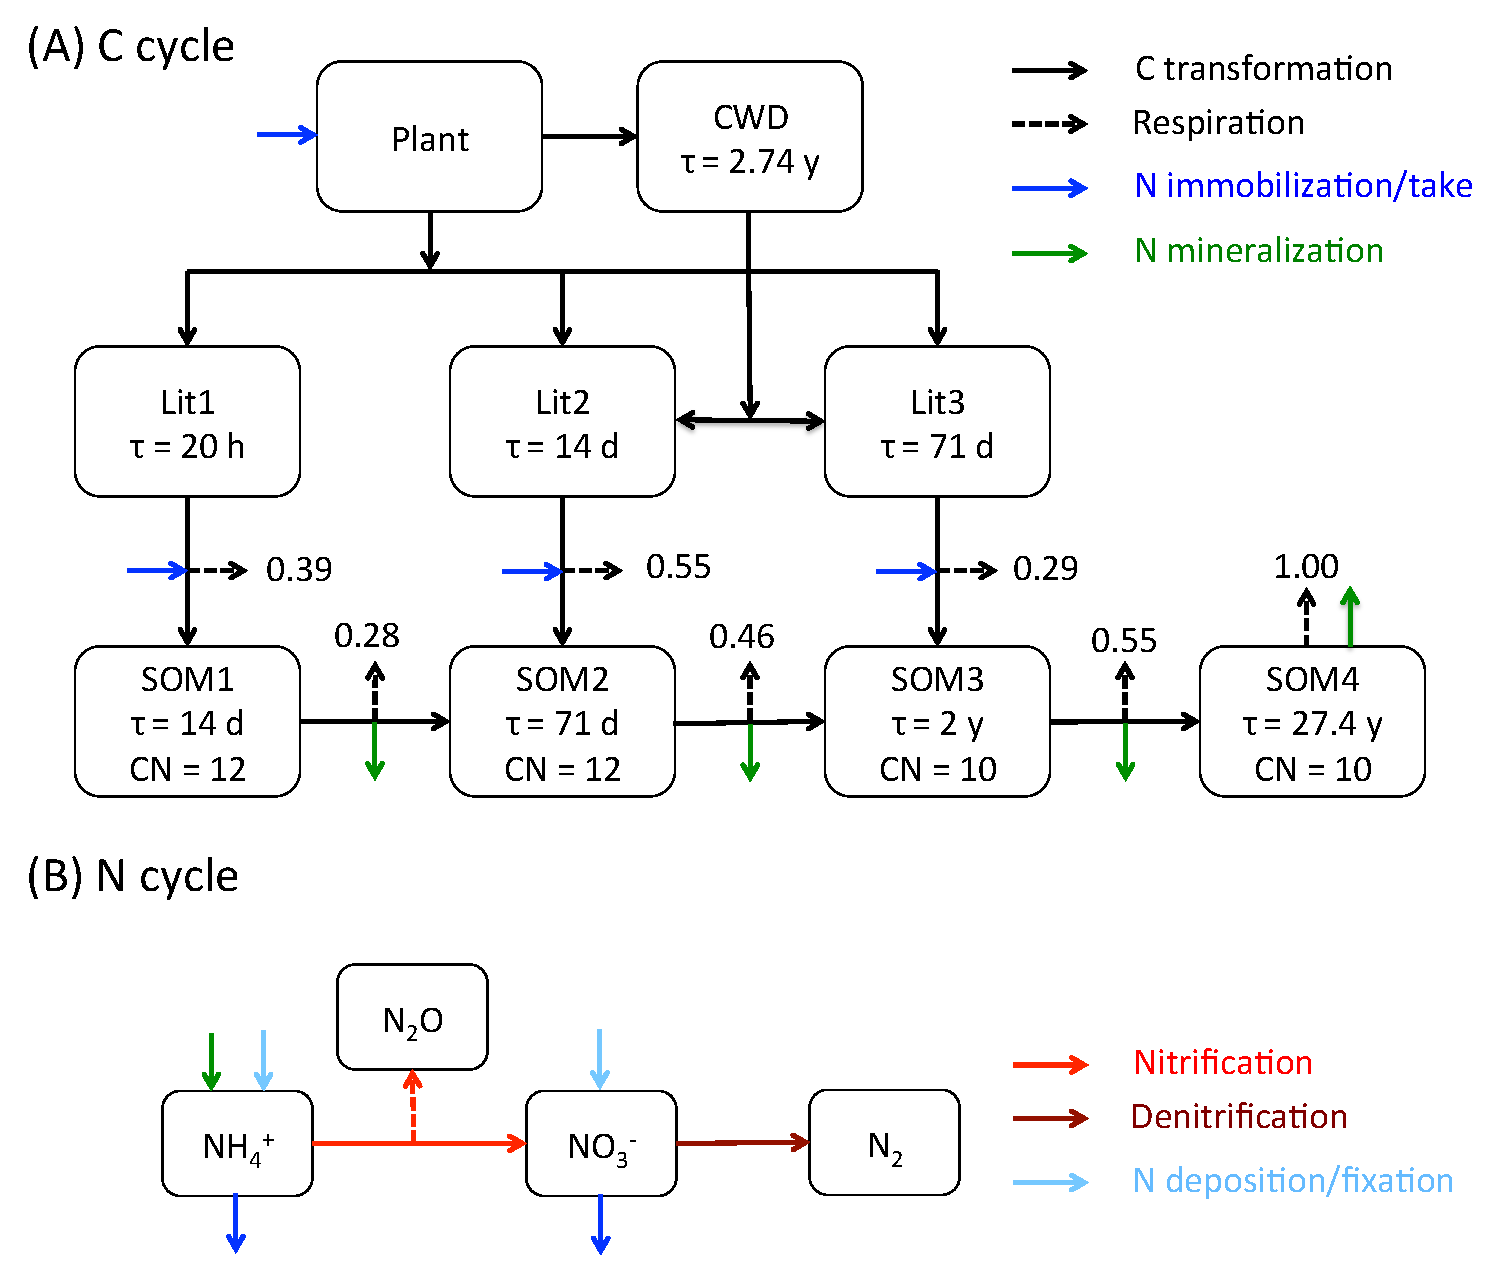
\includegraphics[width=15cm]{../figs/fig01/fig01conceptualmodel.pdf}
\caption{The reaction network for the carbon (A) and nitrogen (B) cycles implemented in this work. The carbon cycle is modified from \citet{Thornton2005} and \citet{Bonan2012}. $\tau$ is the turnover time, and CN is the CN ratio in gC over gN.}
\label{fig:conceptualmodel}
\end{figure}

\begin{figure}[t]
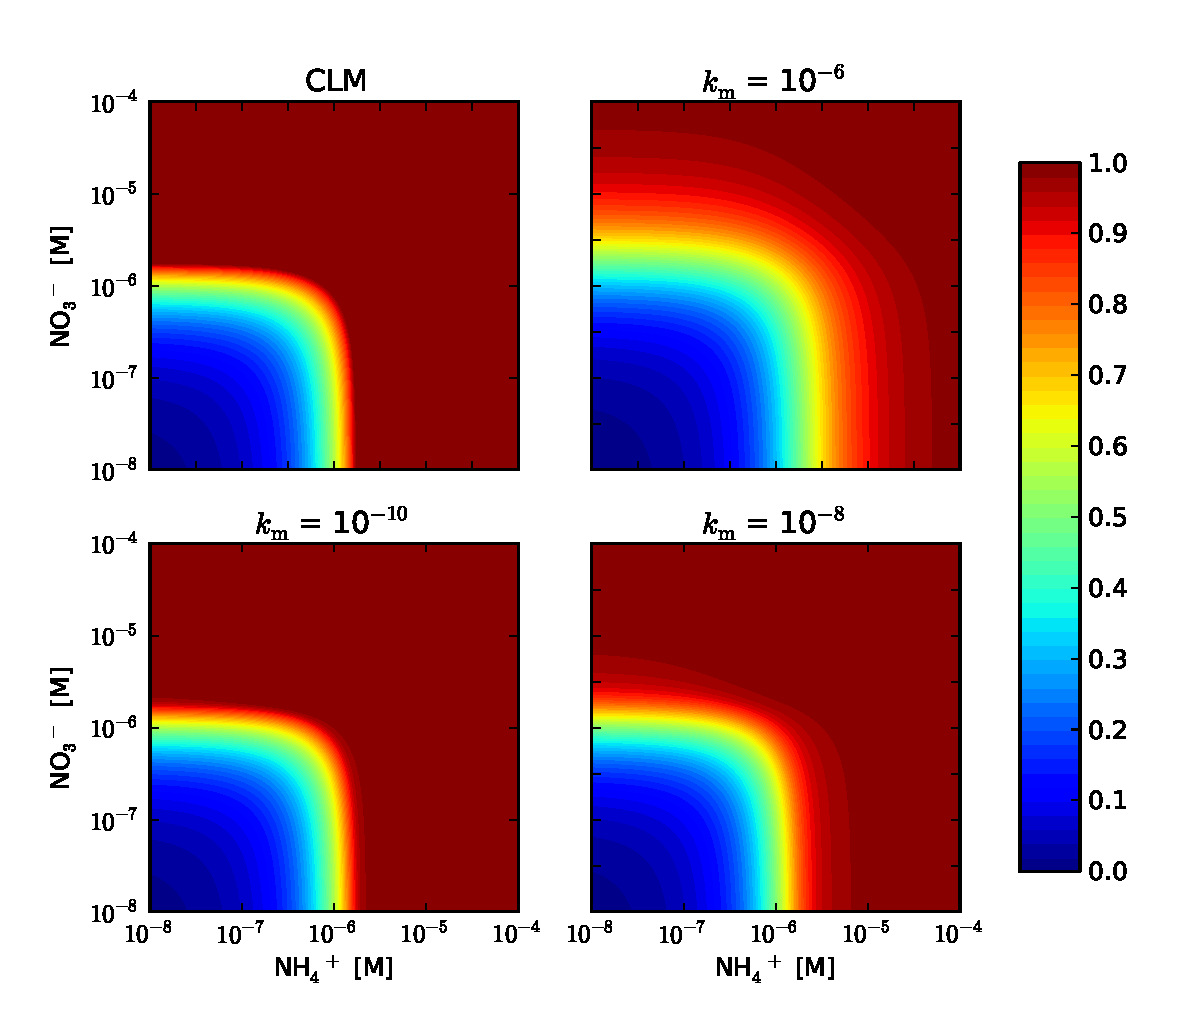
\includegraphics[width=12cm]{../figs/fig05/uptakef.pdf}
\caption{The ratio of uptake and demand ($f_{pi}$) as a
function of concentrations with CLM and representation by Eqs.
(\ref{eq:plantarate}) and (\ref{eq:plantnrate}) in a 0.5 h time step with an
uptake rate of 10$^{-9}$ \unit{M\,s^{-1}}. $f_{pi}$ for the new representation
is less than or equal to that for CLM. The difference decreases with decreasing
half saturation $k_\text{m}$.}
\label{fig:demanddistribution}
\end{figure}

\begin{figure}[t]
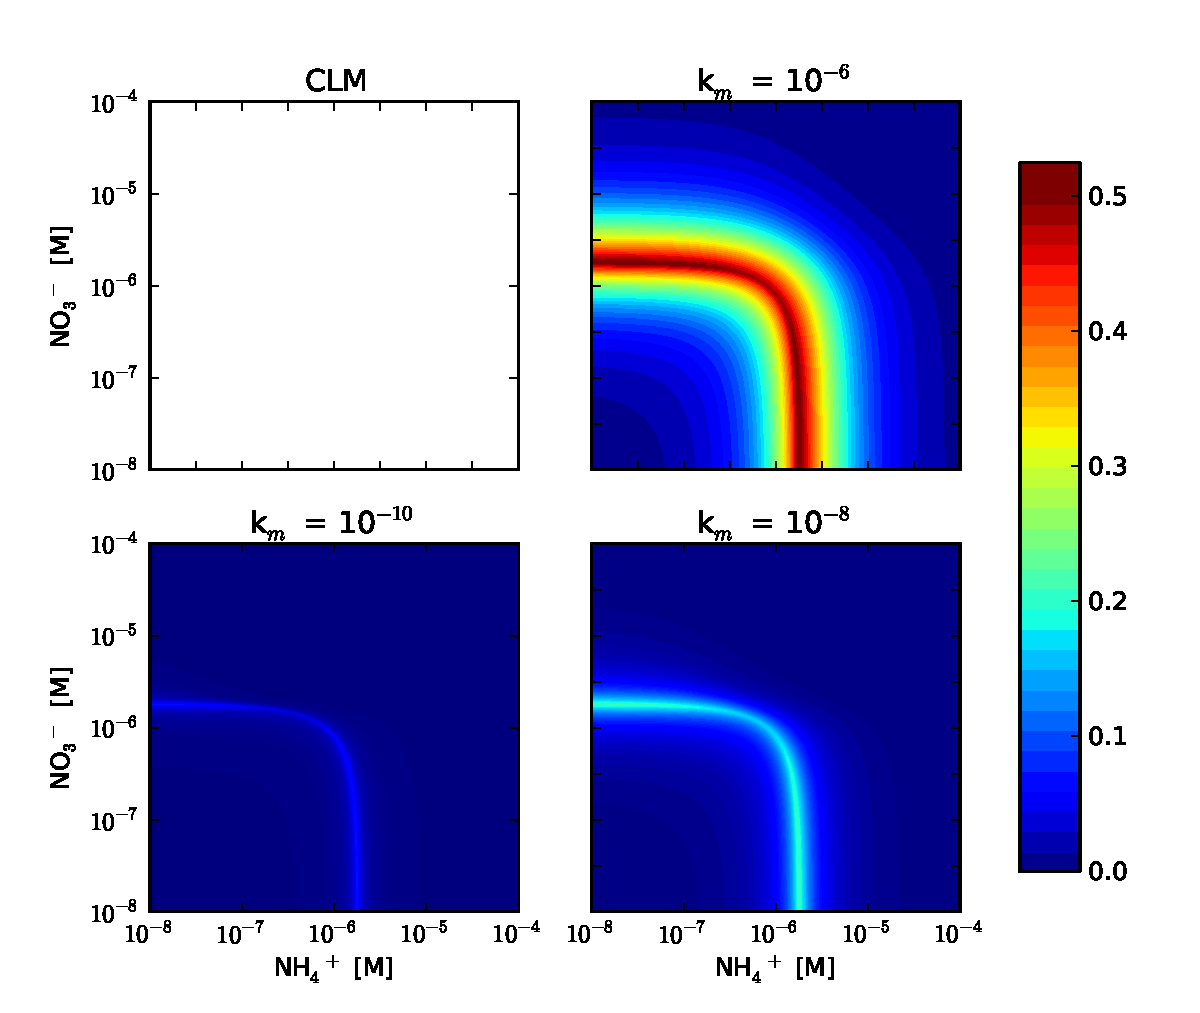
\includegraphics[width=12cm]{../figs/fig06/uptaked.pdf}
\caption{The difference plots for Fig. (\ref{fig:demanddistribution}).}
\label{fig:demanddistributiondiff}
\end{figure}

\begin{figure}[t]
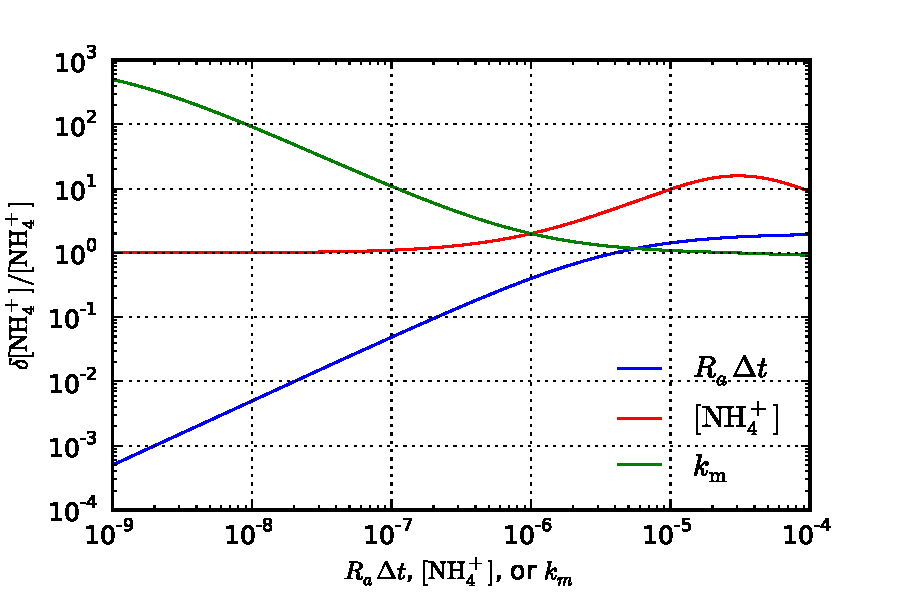
\includegraphics[width=8cm]{../figs/fig07/fig07monodupdate1.pdf}
\caption{The calculated ratio of update over concentration for the first
iteration as a function of time step size ($R_a \Delta t$), initial
concentration (\chem{NH_4^+}), and half saturation ($k_\text{m}$) for solving
$d[\chem{NH_4^+}]/dt=-R_a[\chem{NH_4^+}]/(\chem{NH_4^+} + k_\text{m})$ using
the backward Euler method and Newton-Raphson method. Without scaling back the
update ($\delta$), the concentration in the first iteration step
([\chem{NH_4^+}]$^{k+1,1}$) can go negative if $R_a \Delta$t > 10$^{-5}$,
[\chem{NH_4^+}]$^k$ > 10$^{-6}$, or $k_\text{m}$ < 10$^{-6}$. Unless specified in
the figure, the base case parameters are $R_a \Delta$t = 10$^{-3}$,
\chem{NH_4^+}$^k$ = 10$^{-6}$, and $k_\text{m}$ = 10$^{-6}$.}
\label{fig:monodupdate}
\end{figure}

\begin{figure}[t]
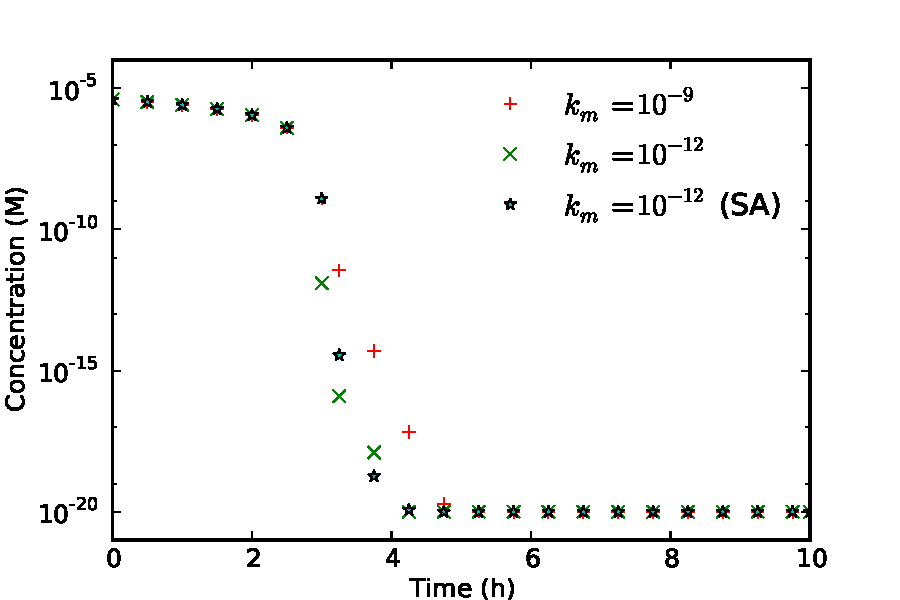
\includegraphics[width=8cm]{../figs/fig08/fig08plantntake1.pdf}
\caption{Influence of half saturation ($k_\text{m}$) on the simulated
\chem{NH_4^+} concentration decrease due to plant uptake. Too small a half
saturation may result in false convergence due to too small an update (scaling
factor) during the iteration. The semi-analytical (SA) solution (Eq.
\ref{eq:monodsemi}) is used for comparison.}
\label{fig:plantntake}
\end{figure}

%\begin{figure}[t]
%\includegraphics[width=8cm]{../figs/fig09/fig09positiveupdate.pdf}
%\caption{Positive update for \chem{NO_3^-} in a plant \chem{NH_4^+} uptake and
%nitrification test problem as a function of \chem{NH_4^+} concentration
%[\chem{NH_4^+}], plant uptake rate $R_a$, nitrification rate coefficient, and
%half saturation for plant uptake. Unless specified in the figure, the base
%parameter values are: \chem{NH_4^+} concentration 10$^{-7}$ \unit{M}, plant
%uptake rate 10$^{-7}$ \unit{mol\,m^{-3}s^{-1}}, nitrification rate coefficient
%10$^{-6}$ \unit{s^{-1}}, half saturation 10$^{-8}$ \unit{M}, and time step
%size 0.5 \unit{h}. The dash dot lines correspond to the cases when the
%nitrification rate is also down regulated with the same Monod substrate
%limiting function as plant uptake.}
%\label{fig:positiveupdate}
%\end{figure}

\begin{figure}[t]
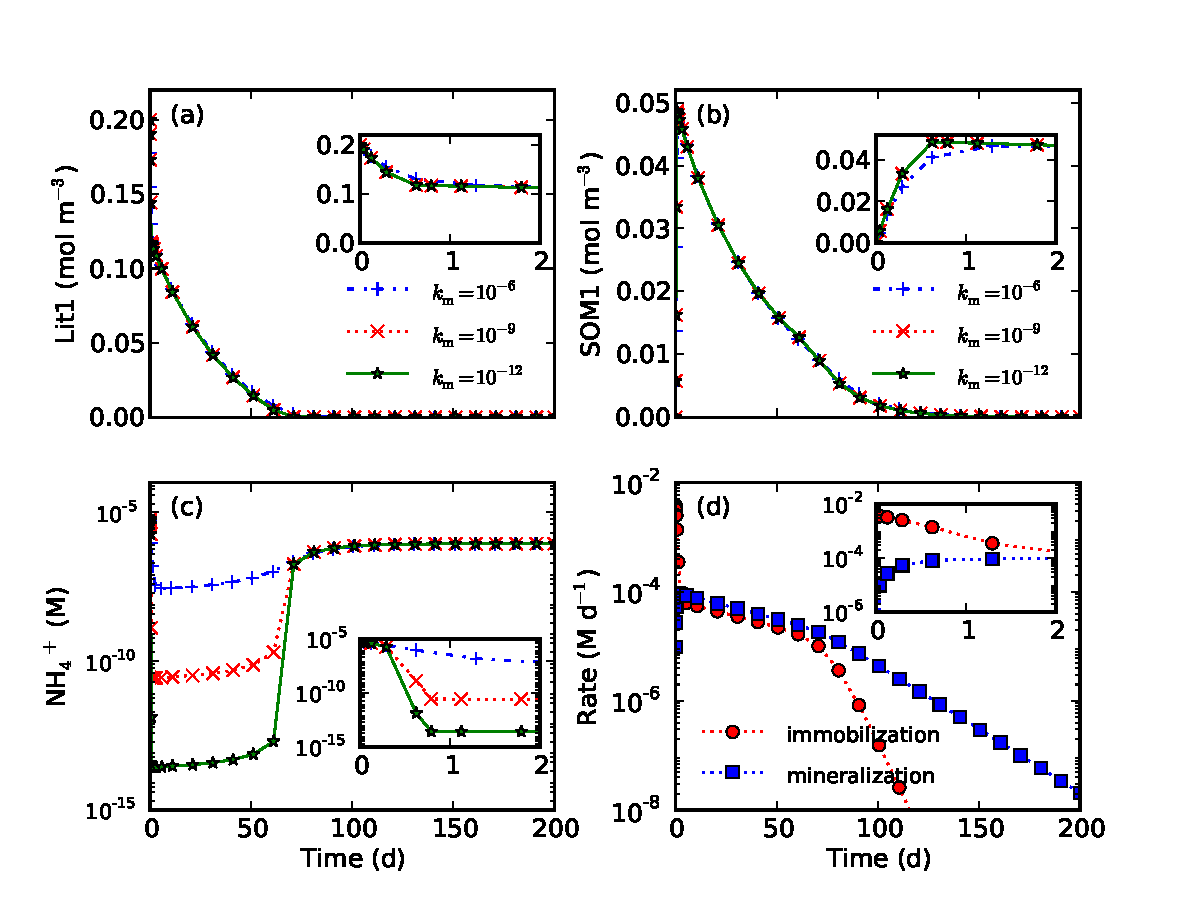
\includegraphics[width=15cm]{../figs/fig09/figdecomp.pdf}
\caption{Influence of half saturation $k_m$ on decomposition that involves both
nitrogen immobilization and mineralization. Smaller half saturation can result
in lower nitrogen concentration (d) but does not substantially impact the
calculated concentrations other than \chem{NH_4^+} (a,b,c).}
\label{fig:decomp}
\end{figure}

\begin{figure}[t]
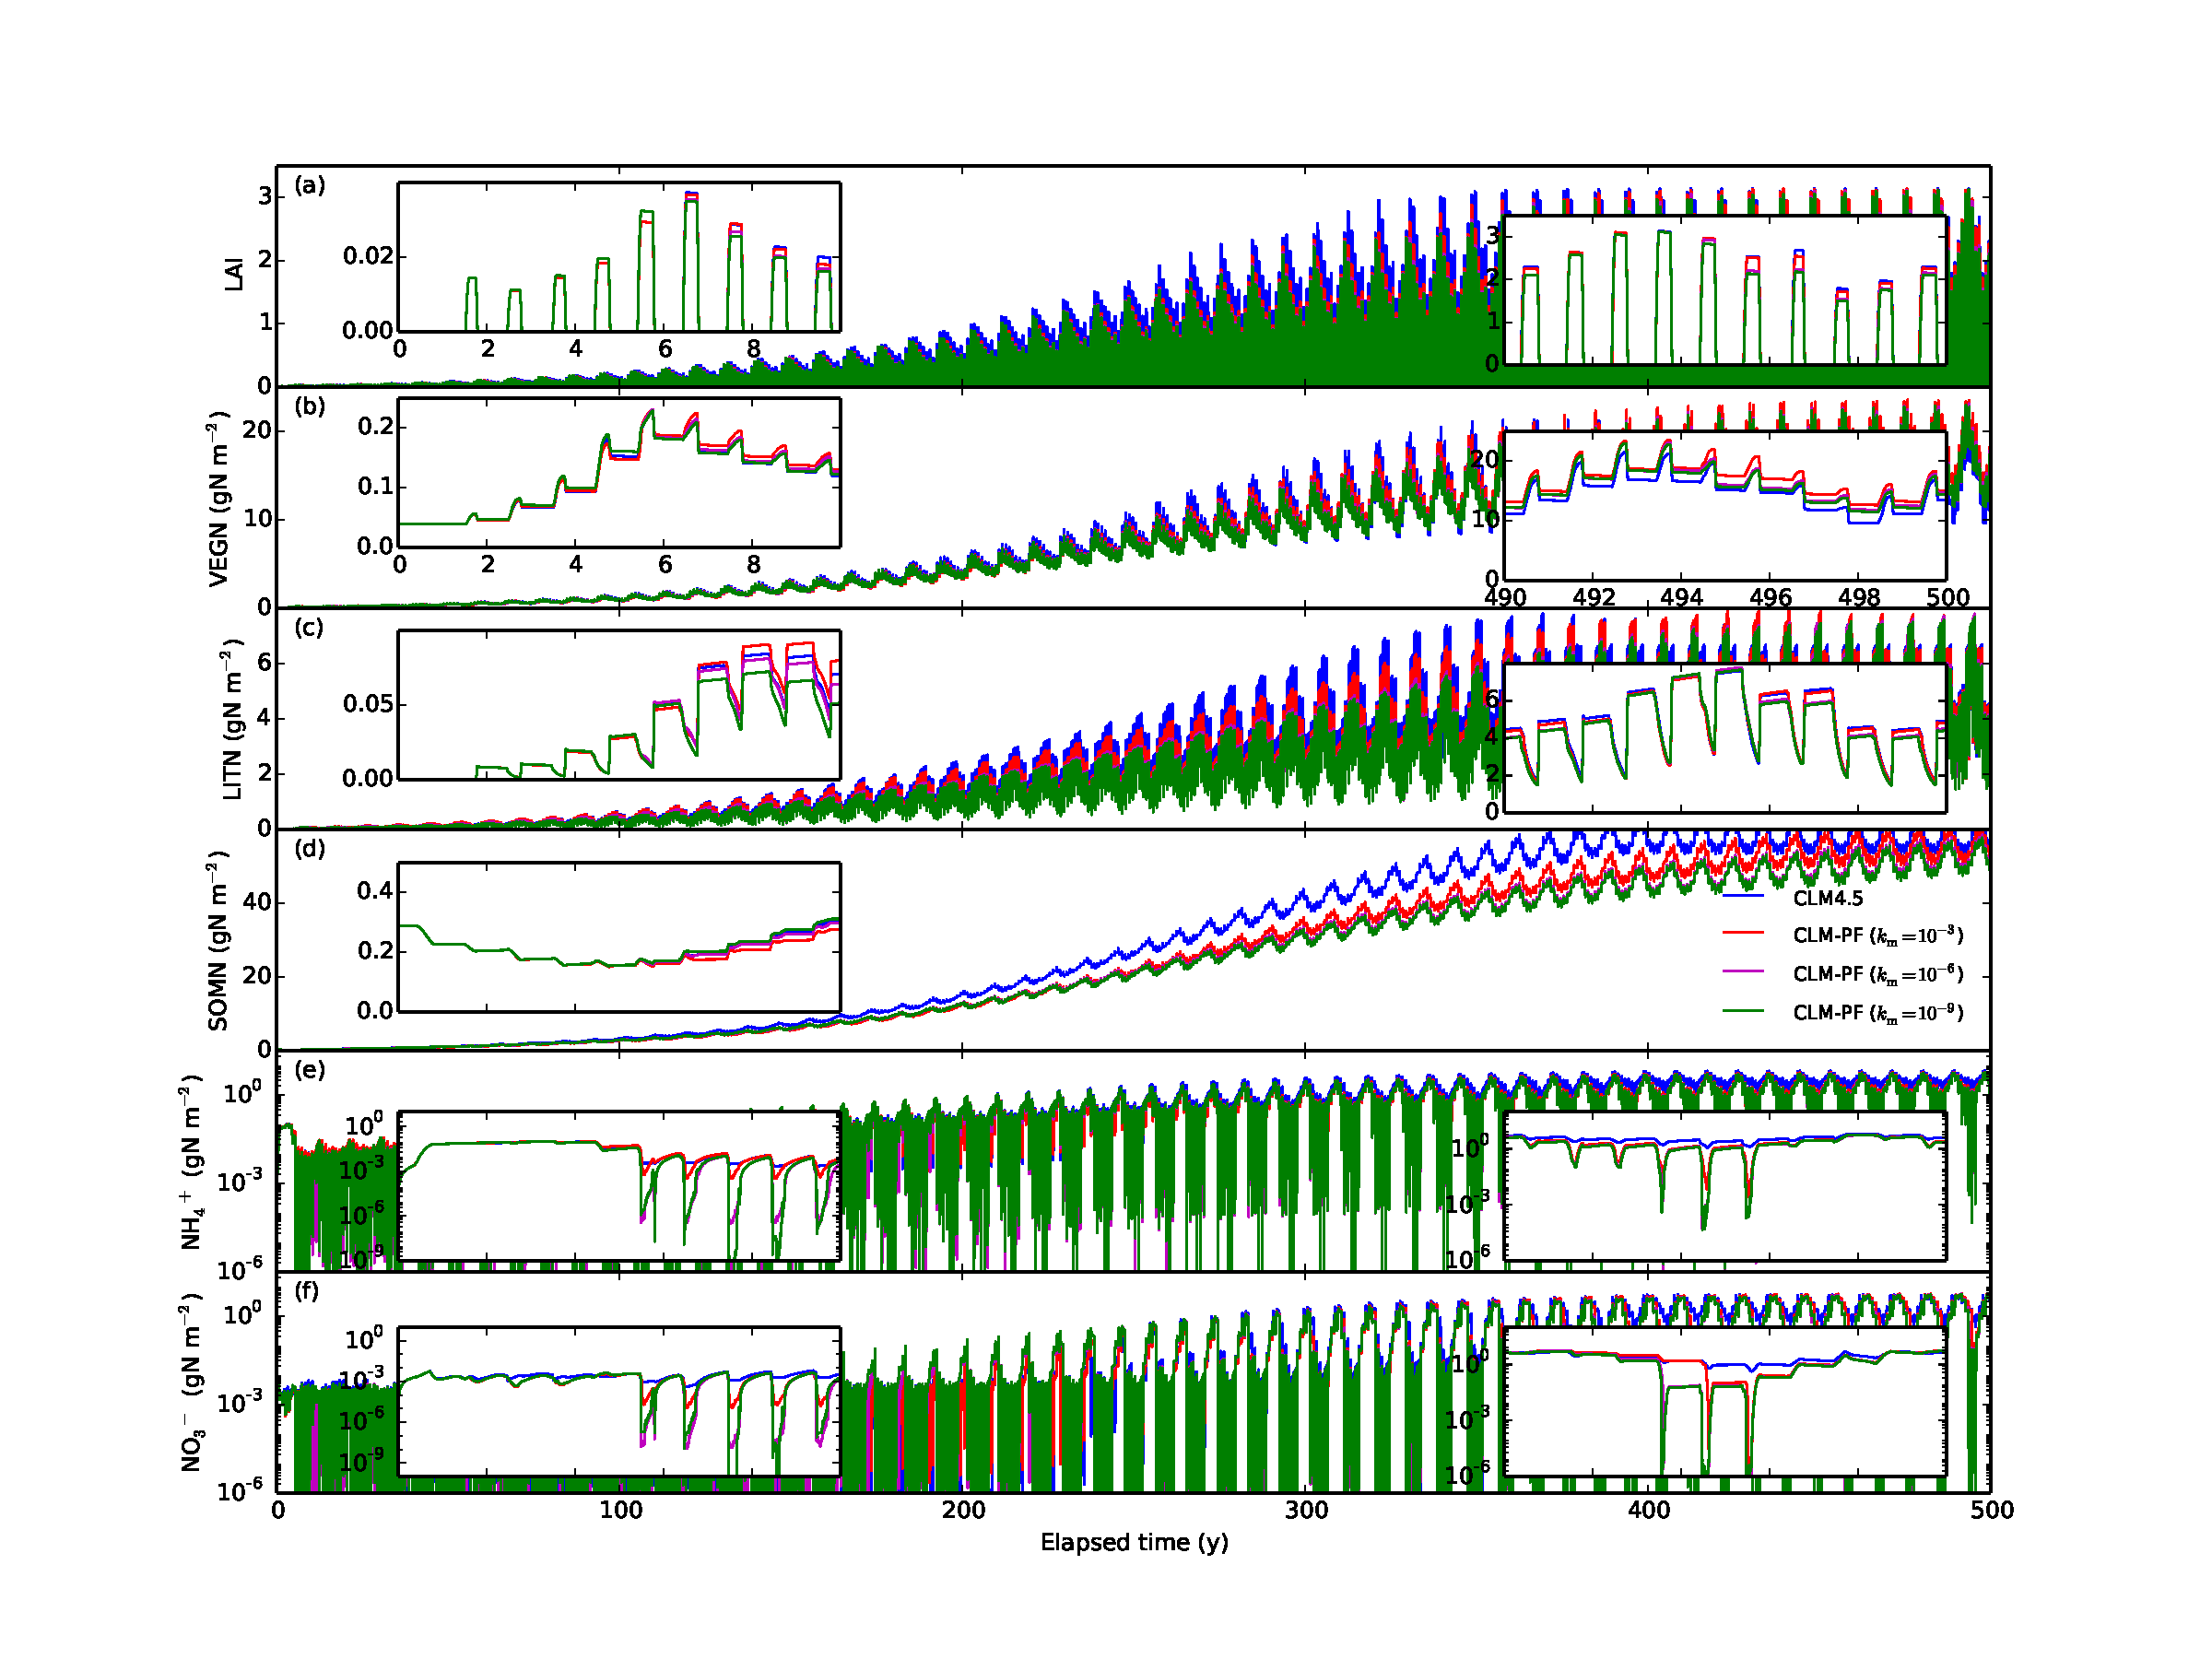
\includegraphics[width=1.0\textwidth]{../figs/fig10/brw500yl.pdf}
\caption{Calculated LAI and nitrogen distribution among vegetation, litter,
SOM, \chem{NH_4^+}, and \chem{NO_3^-} pools in spin-up simulations for the US-Brw
site. Log transformation is used to enforce nonnegativity for CLM-PFLOTRAN.}
\label{fig:brw500yl}
\end{figure}

\begin{figure}[t]
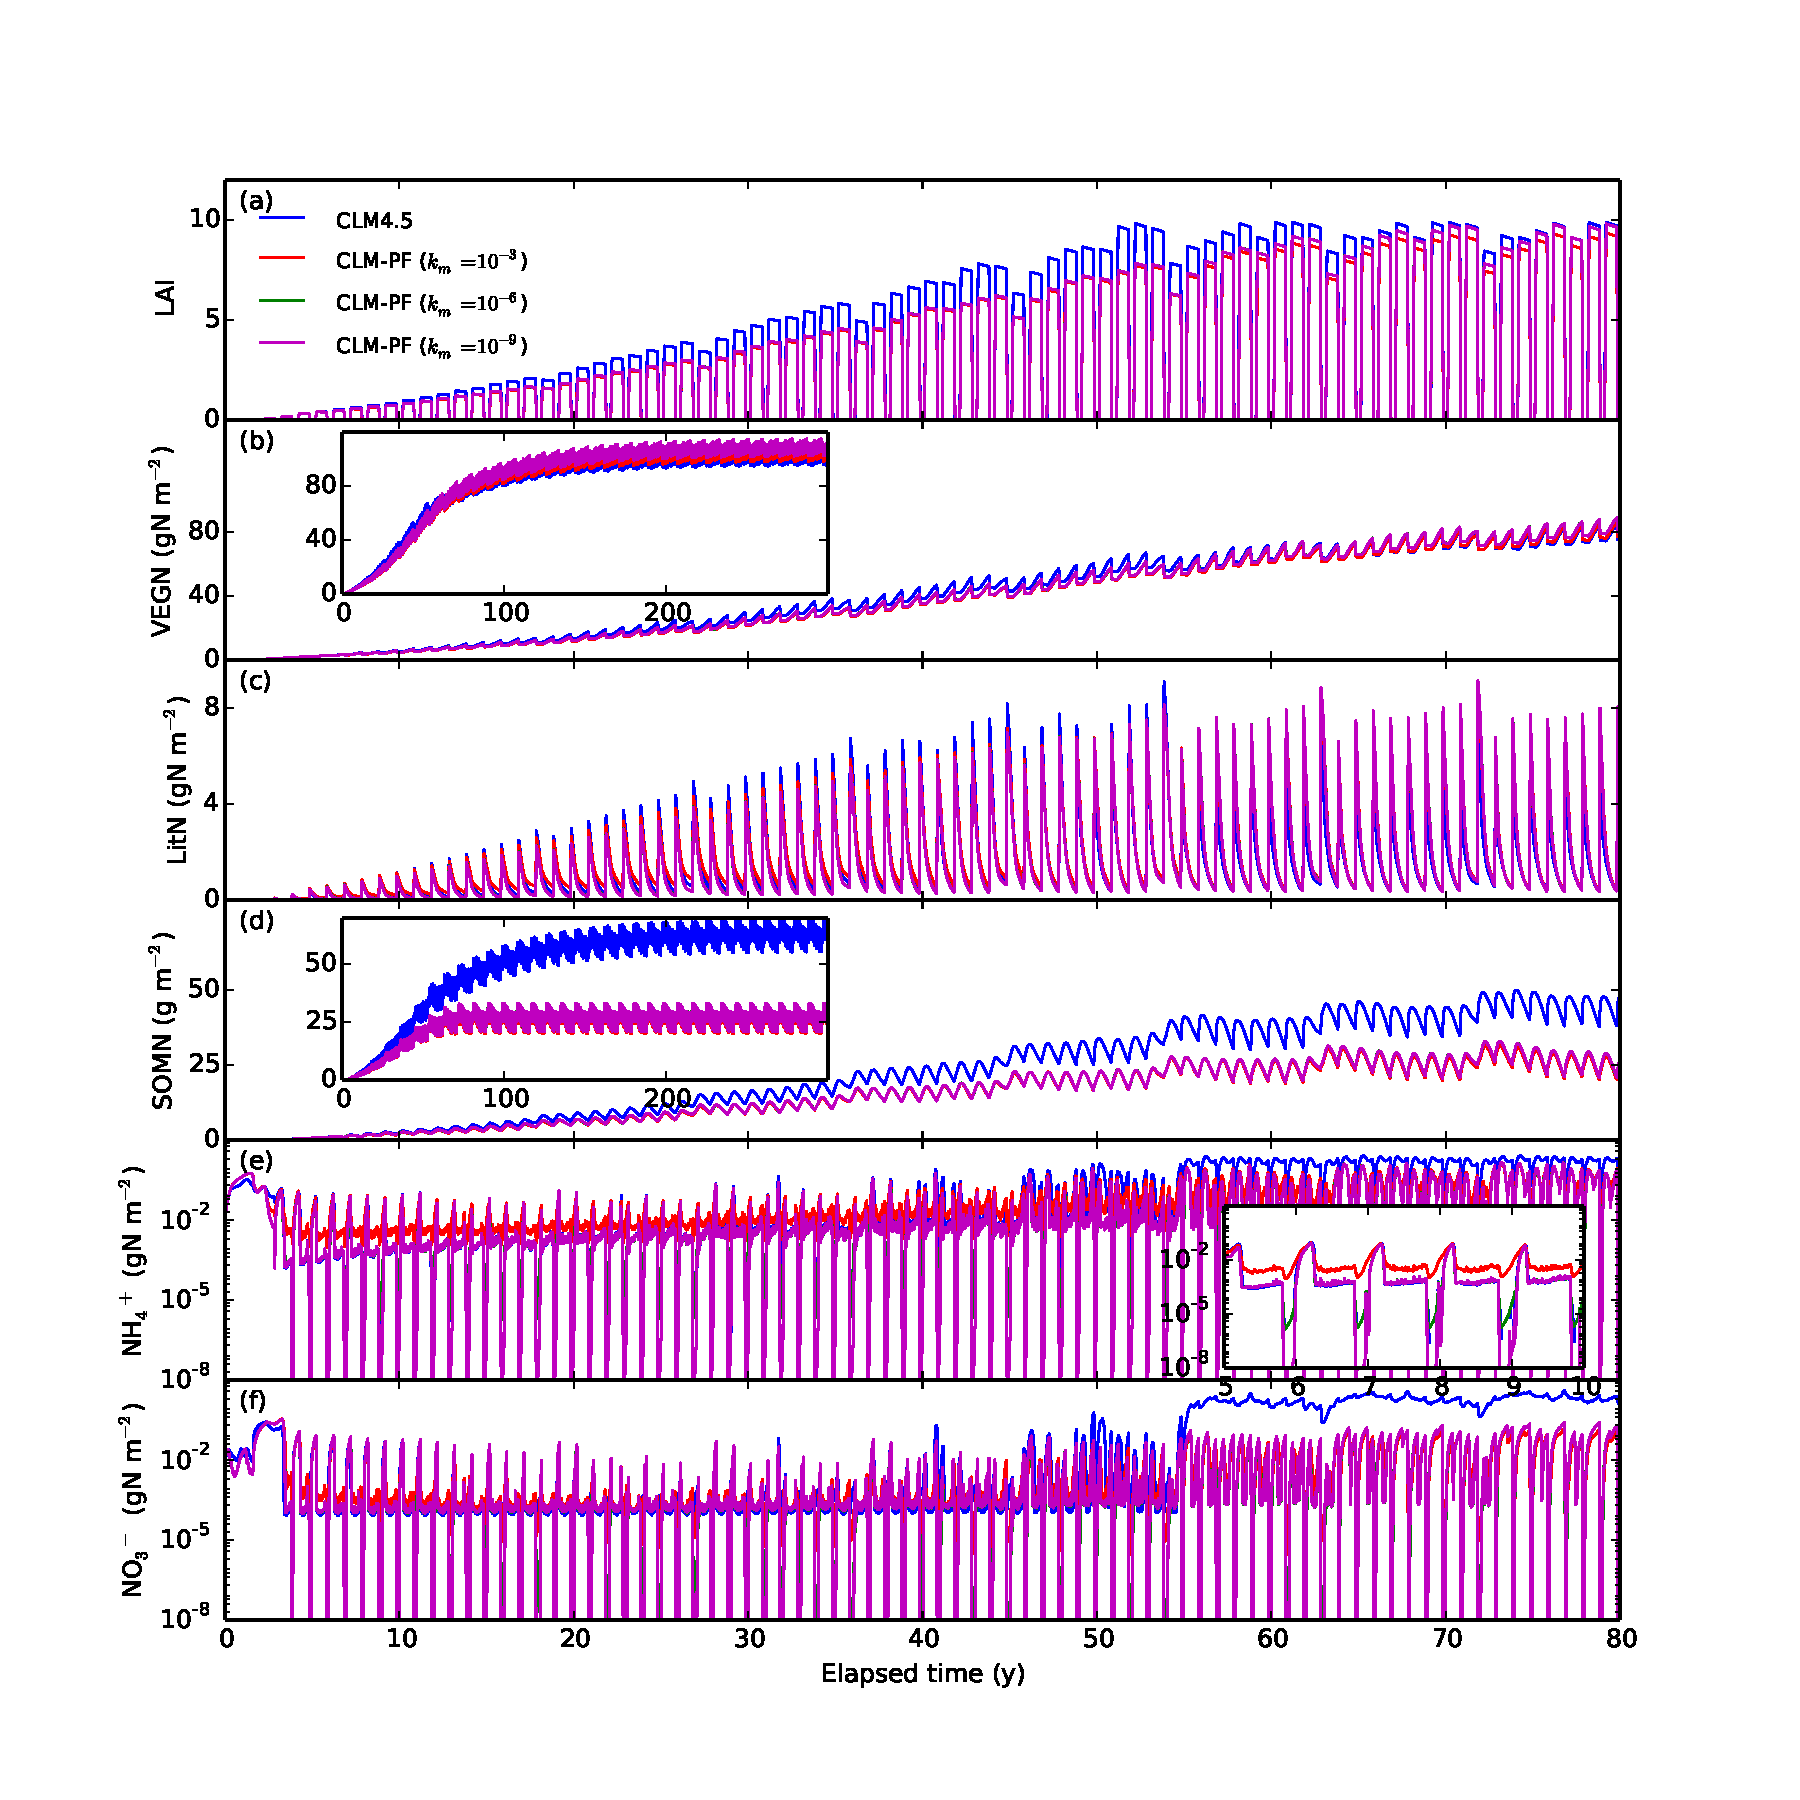
\includegraphics[width=1.0\textwidth]{../figs/fig11/pit300yl.pdf}
\caption{Calculated LAI and nitrogen distribution among vegetation, litter,
SOM, \chem{NH_4^+}, and \chem{NO_3^-} pools in spin-up simulations for US-WBW
site. Log transformation is used to enforce nonnegativity for CLM-PFLOTRAN
calculations.}
\label{fig:pit300yl}
\end{figure}

\begin{figure}[t]
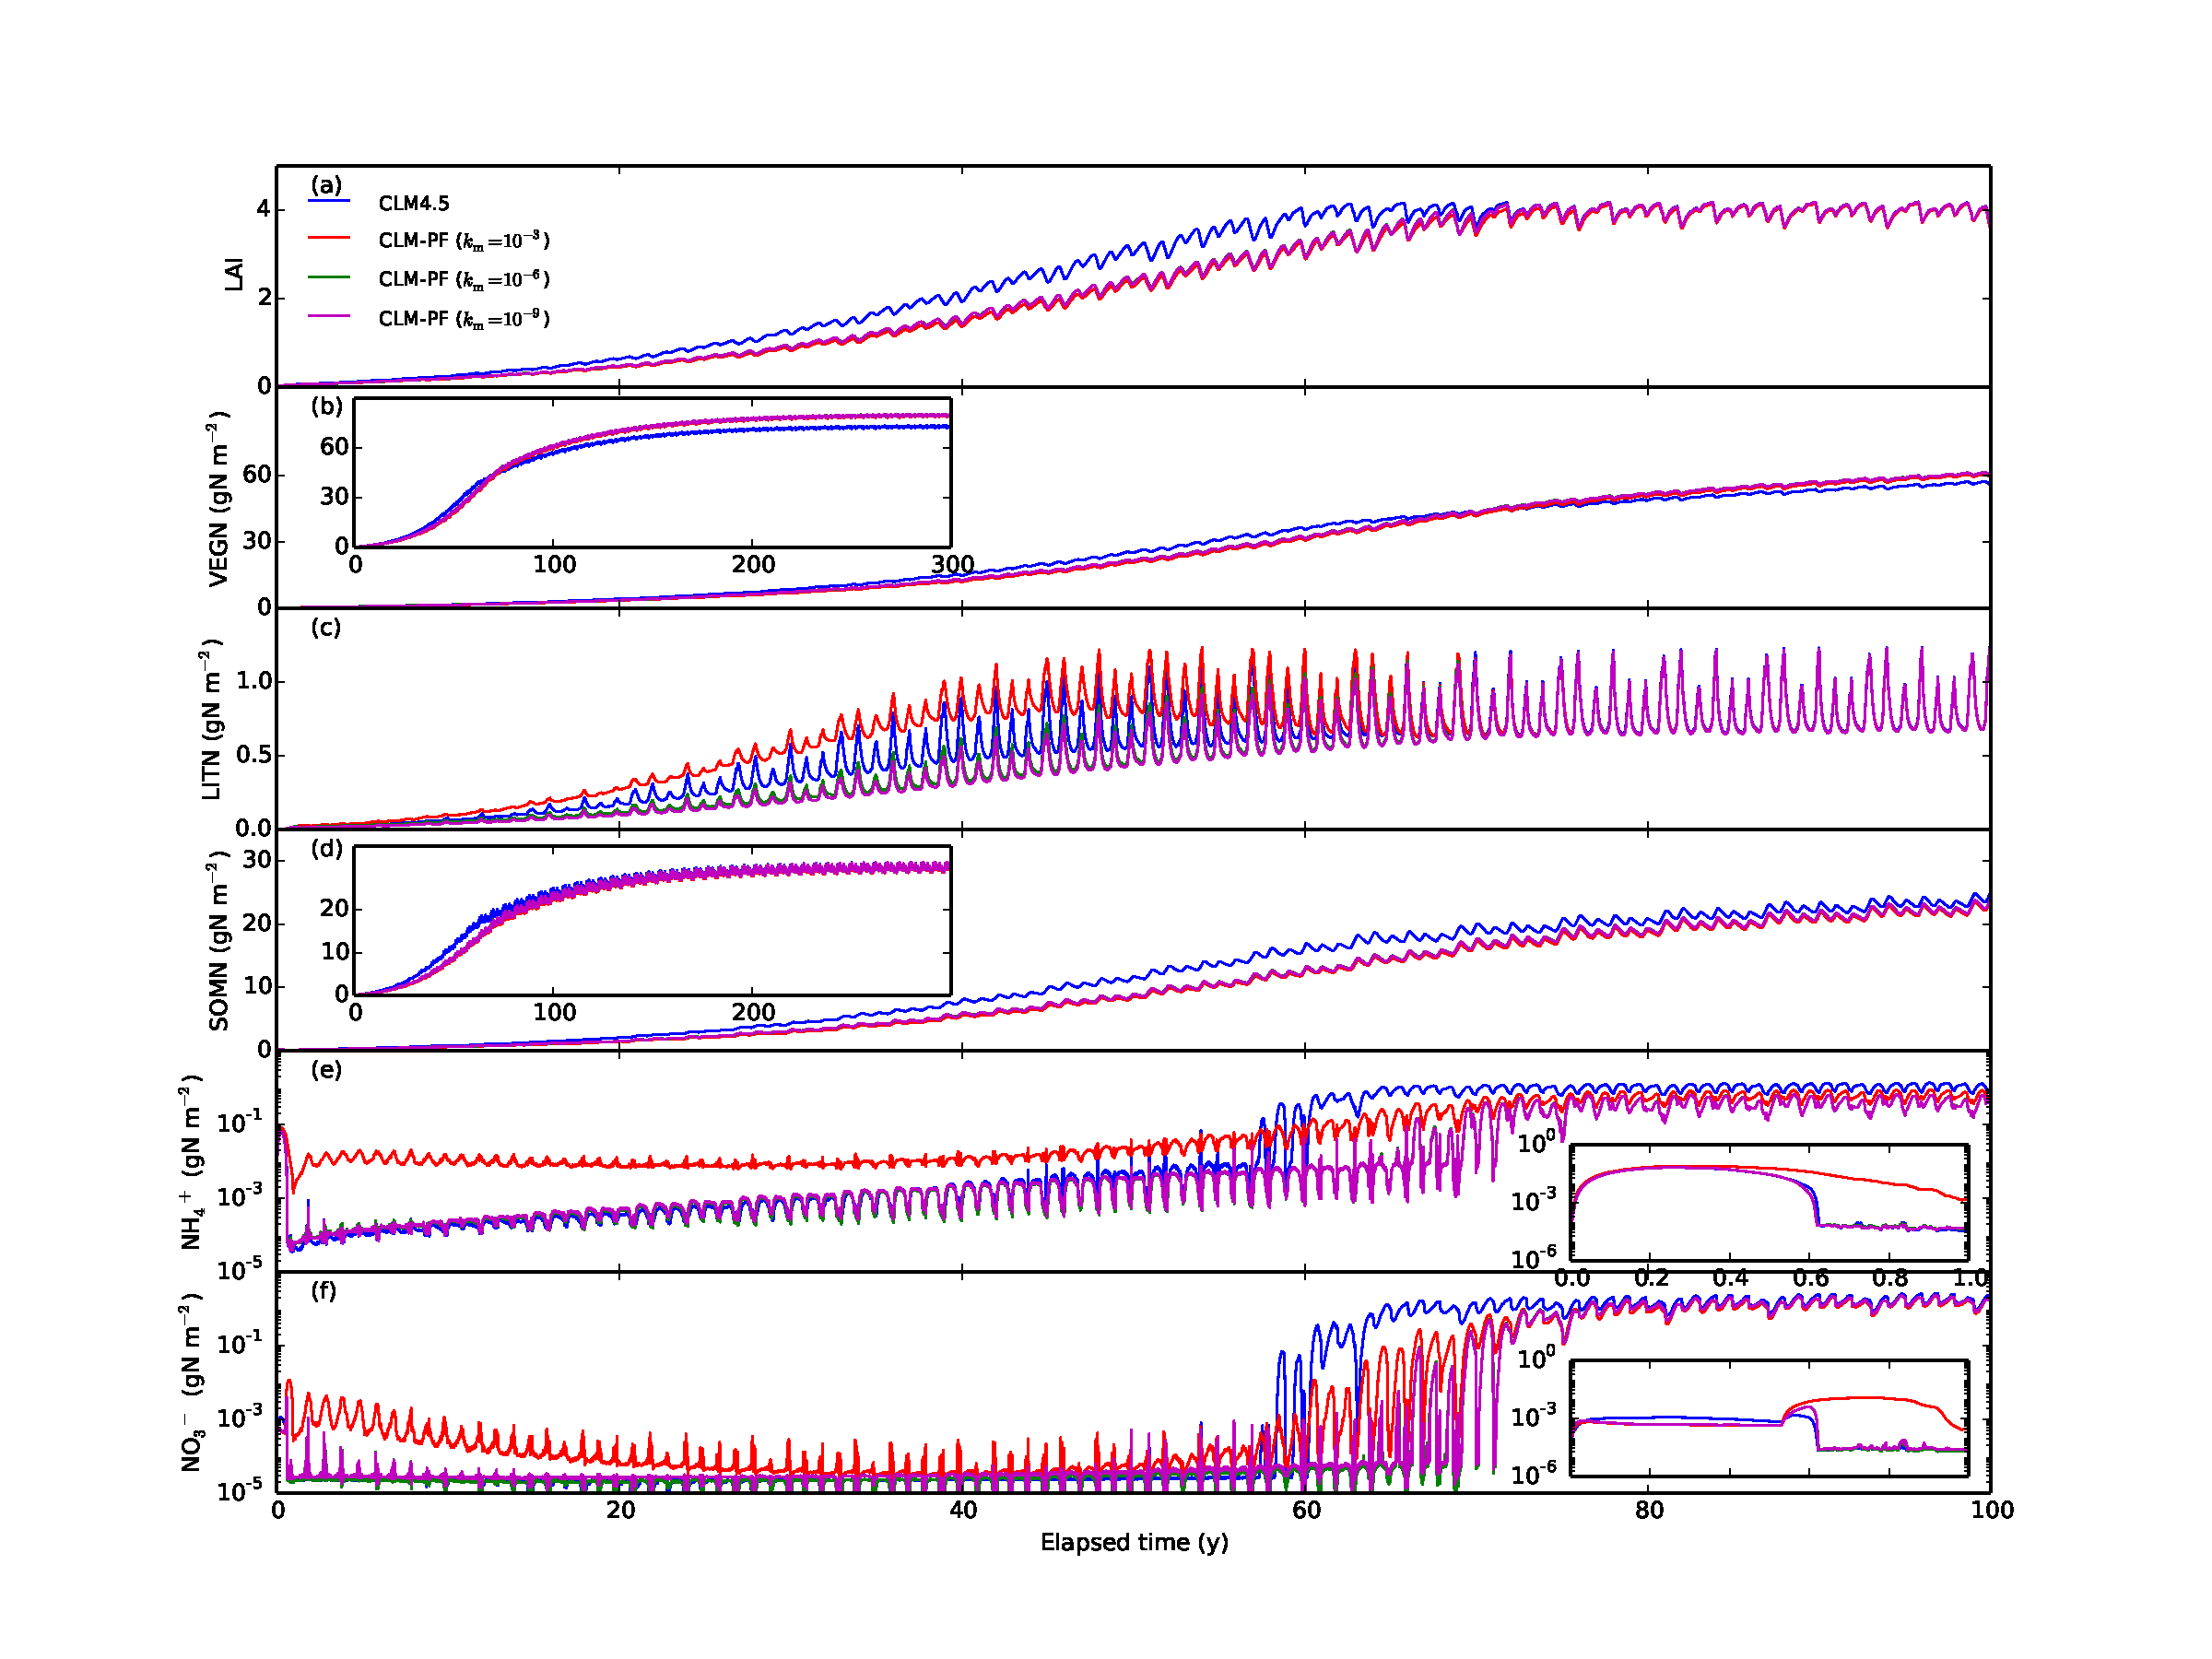
\includegraphics[width=1.0\textwidth]{../figs/fig12/cax300yl.pdf}
\caption{Calculated LAI and nitrogen distribution among vegetation, litter,
SOM, \chem{NH_4^+}, and \chem{NO_3^-} pools in spin-up simulations for BR-Cax
site. Log transformation is used to enforce nonnegativity for CLM-PFLOTRAN
calculations.}
\label{fig:cax300yl}
\end{figure}

\begin{figure}[t]
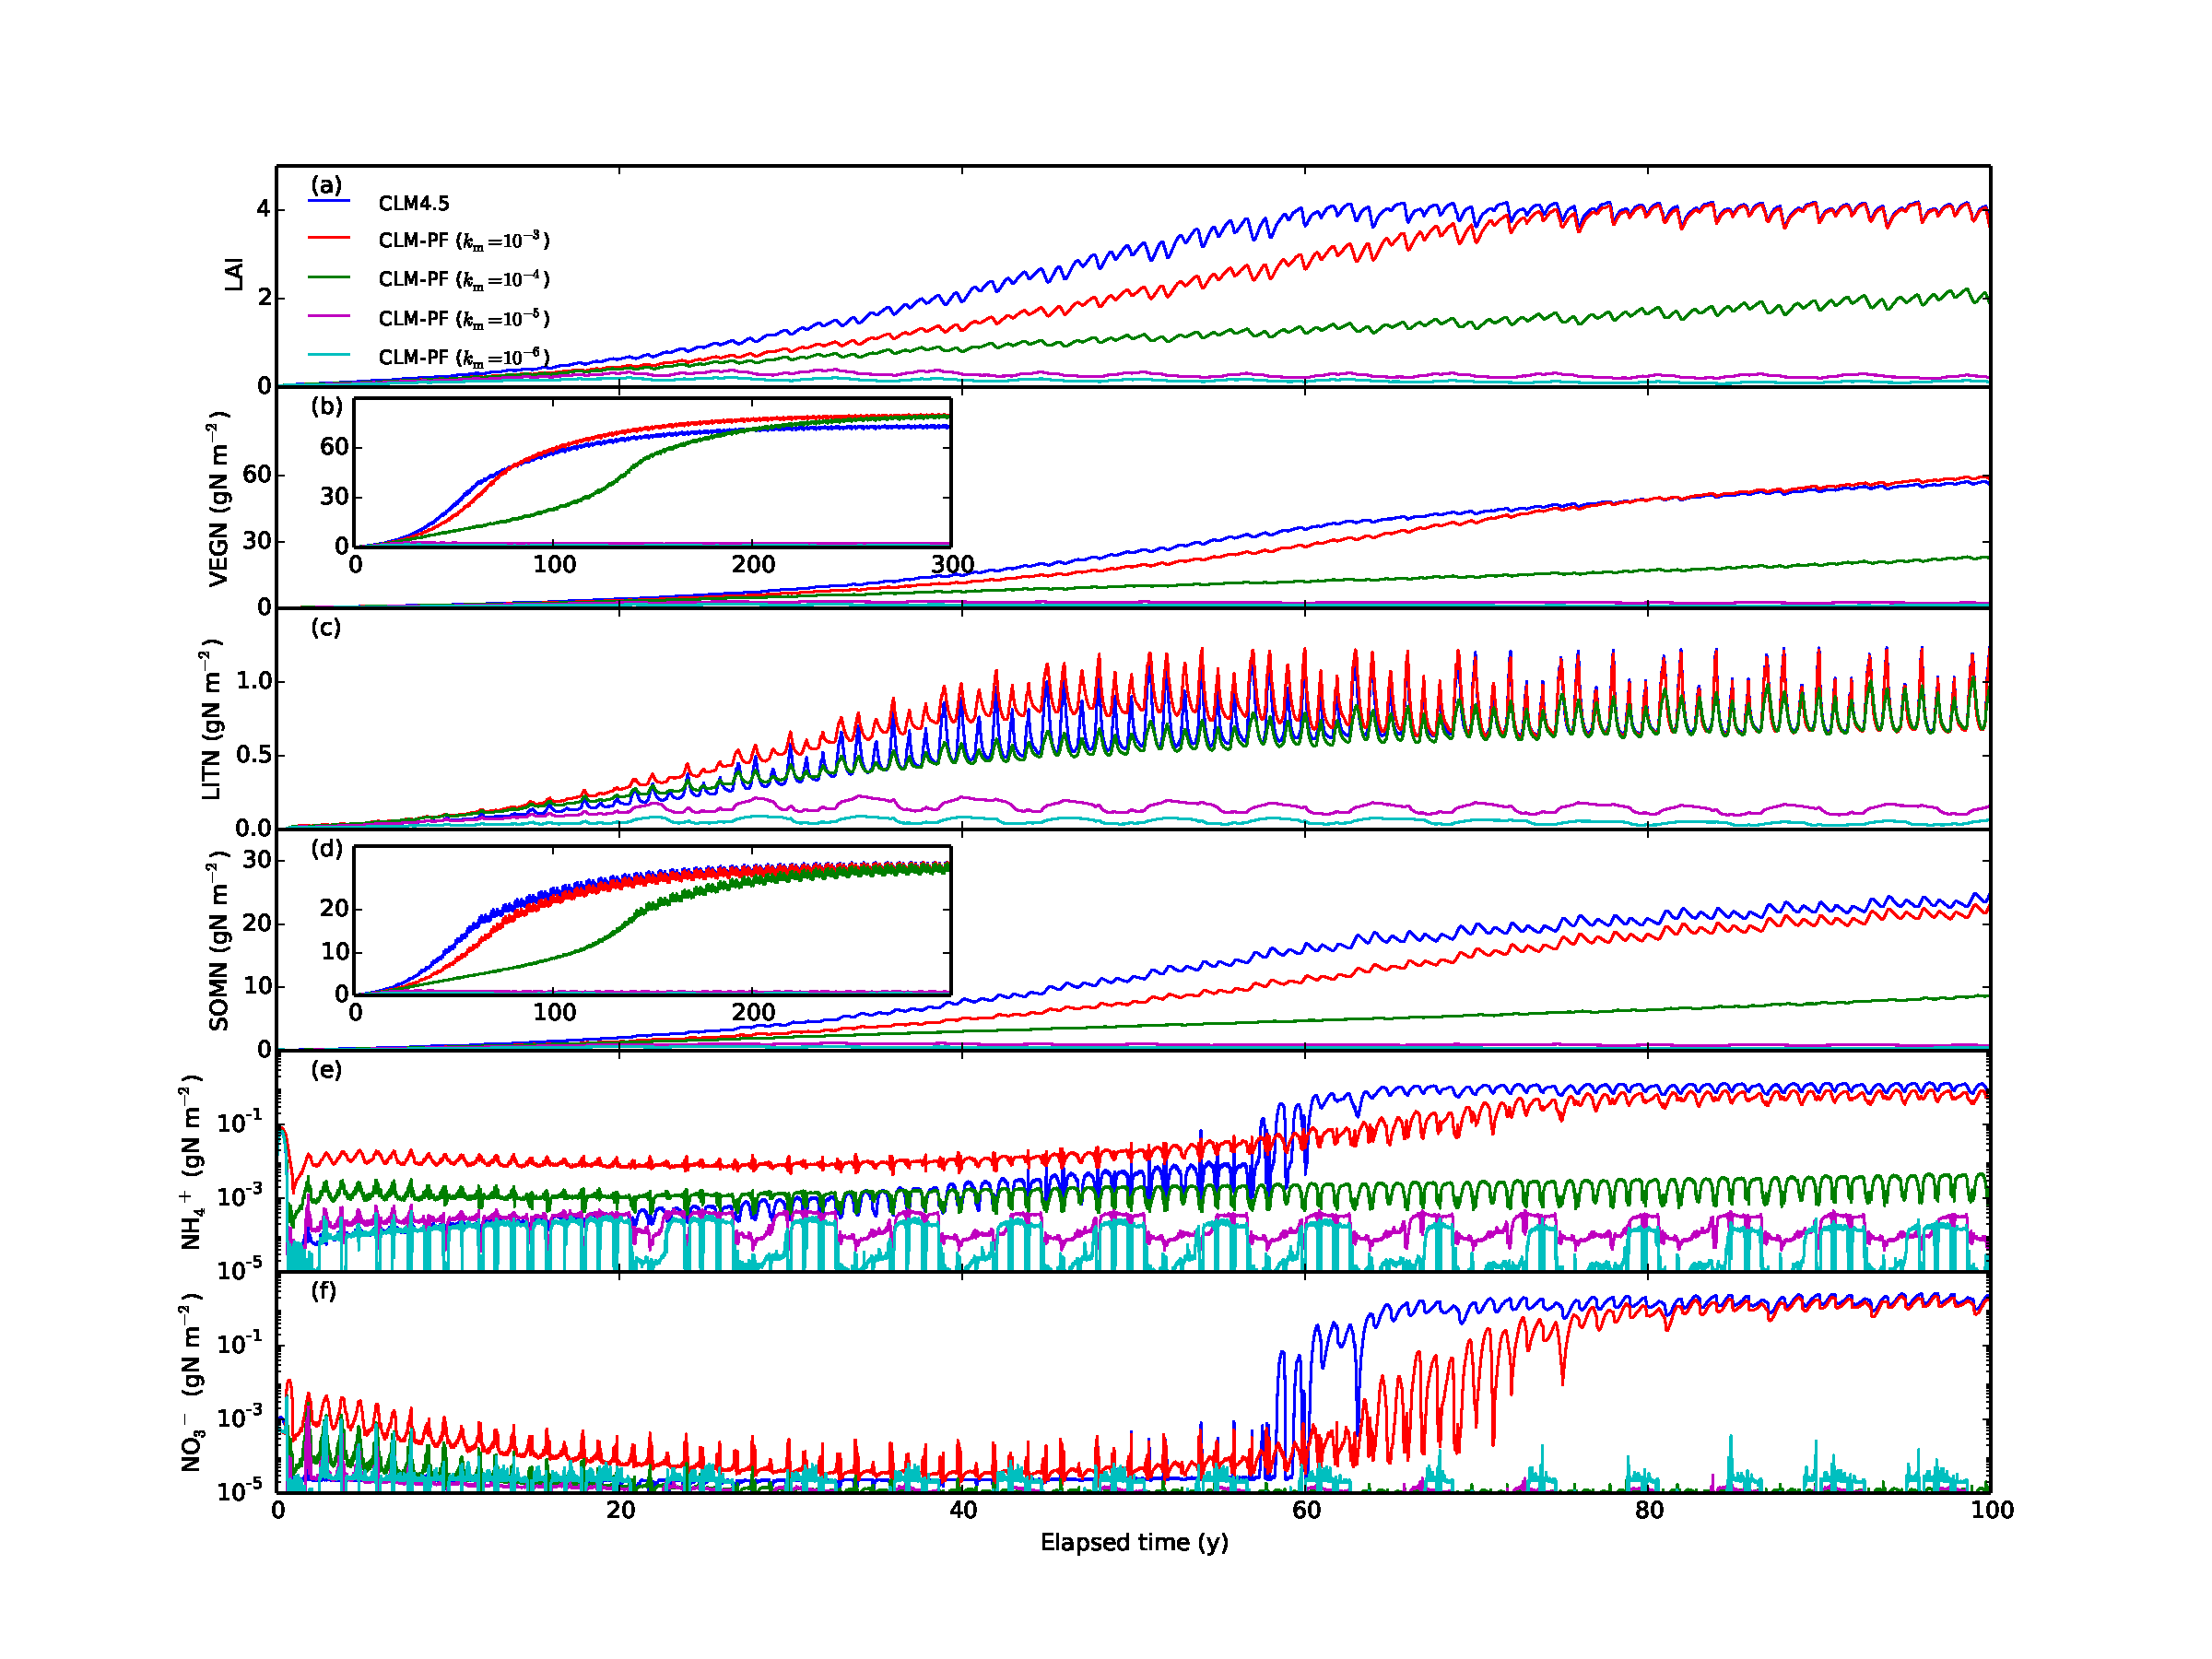
\includegraphics[width=1.0\textwidth]{../figs/fig13/cax300y.pdf}
\caption{Calculated LAI and nitrogen distribution among vegetation, litter,
SOM,  \chem{NH_4^+}, and \chem{NO_3^-} pools in spin-up simulations for BR-Cax
site. Scaling back update in each iteration is used enforce nonnegativity for
CLM-PFLOTRAN.}
\label{fig:cax300y}
\end{figure}

\begin{figure}[t]
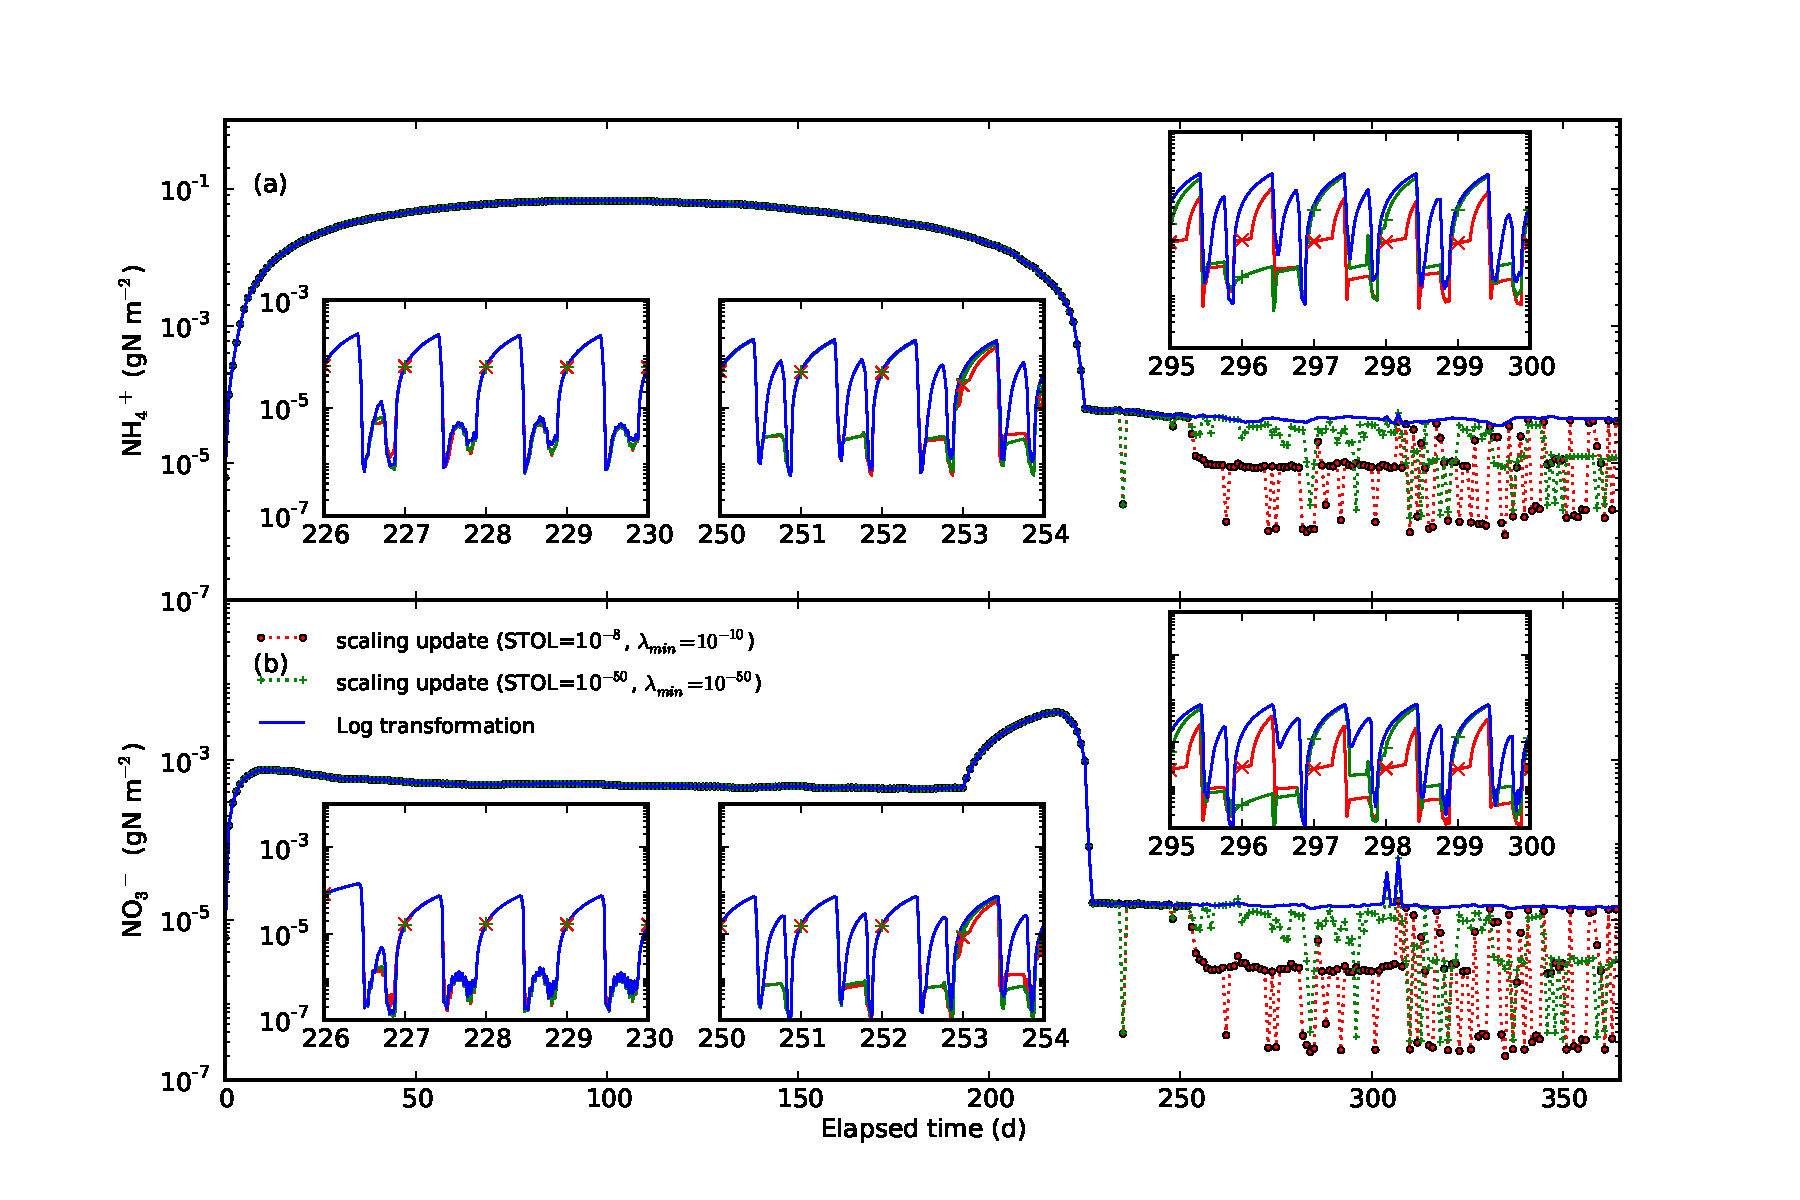
\includegraphics[width=1.0\textwidth]{../figs/fig14/cax1y2.pdf}
\caption{Calculated \chem{NH_4^+} and \chem{NO_3^-} concentration in the first
year using SU (scaling update) vs. LT (log transformation) in the spin-up
simulation for BR-Cax site with $k_\text{m} = 10^{-6}$ \unit{mol\,m^{-3}}.
``skip derivative'' refers to not including the derivatives for the reaction
(\ref{rxn:nitr2n2o}) with rate (Eq. \ref{eq:nitr2n2odecomp}) in
the entries for \chem{N_2Od} in the Jacobian matrix.}
\label{fig:cax1y}
\end{figure}

\begin{figure}[t]
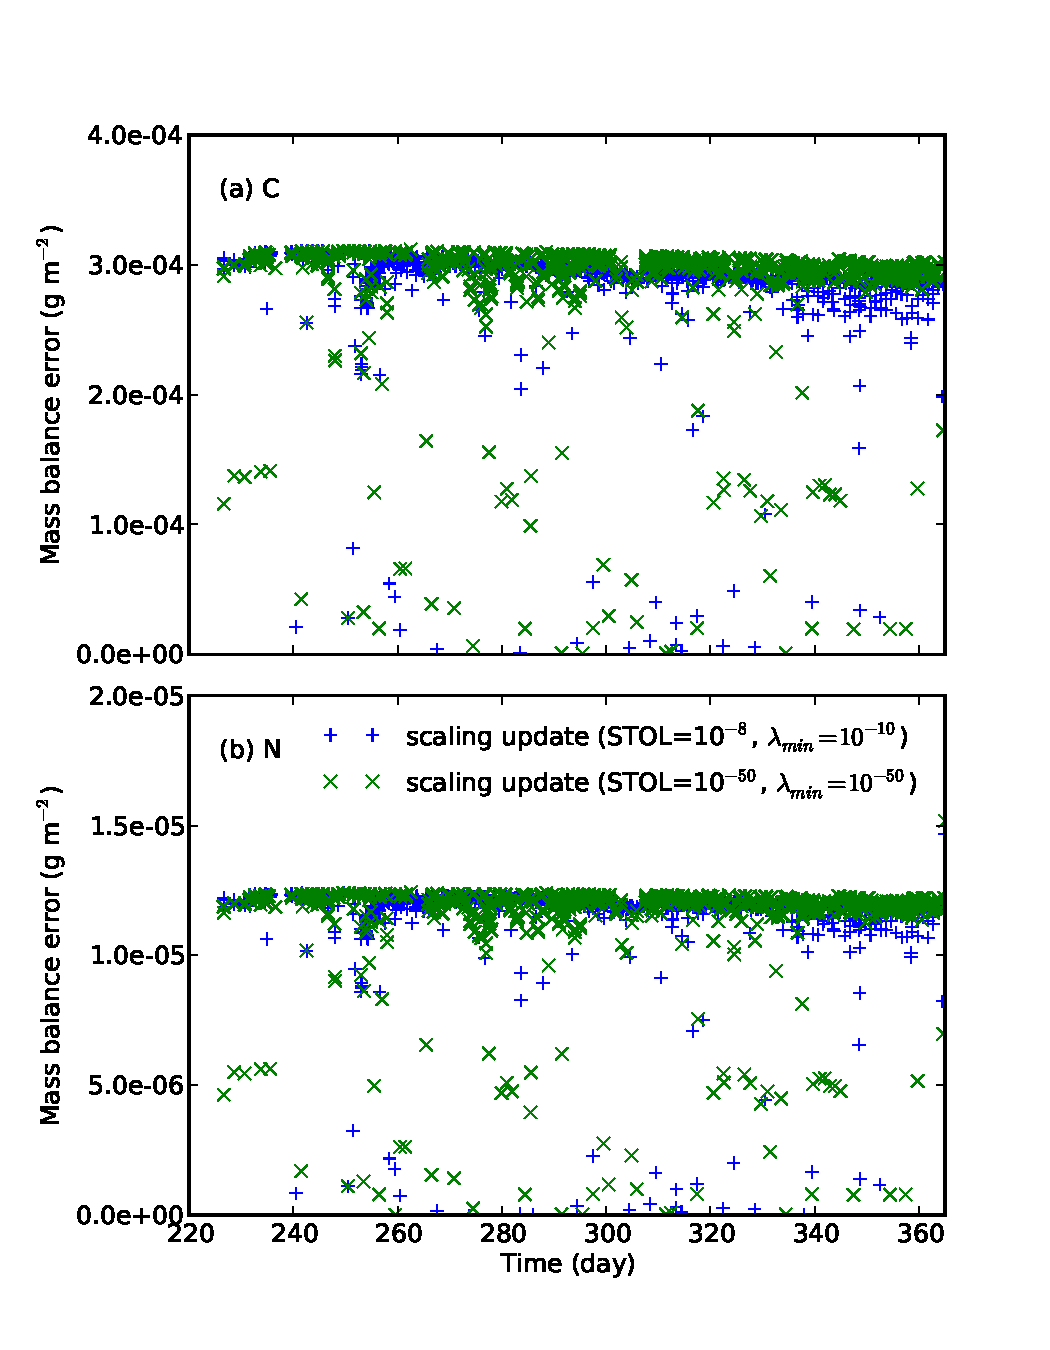
\includegraphics[width=7.5cm]{../figs/fig17/mbe.pdf}
\caption{Mass balance error for (a) C and (b) N in the first year where SU with
$k_m = 10^{-6}$ \unit{mol\,m^{-3}} is used for the tropical site.}
\label{fig:mbe}
\end{figure}

\begin{figure}[t]
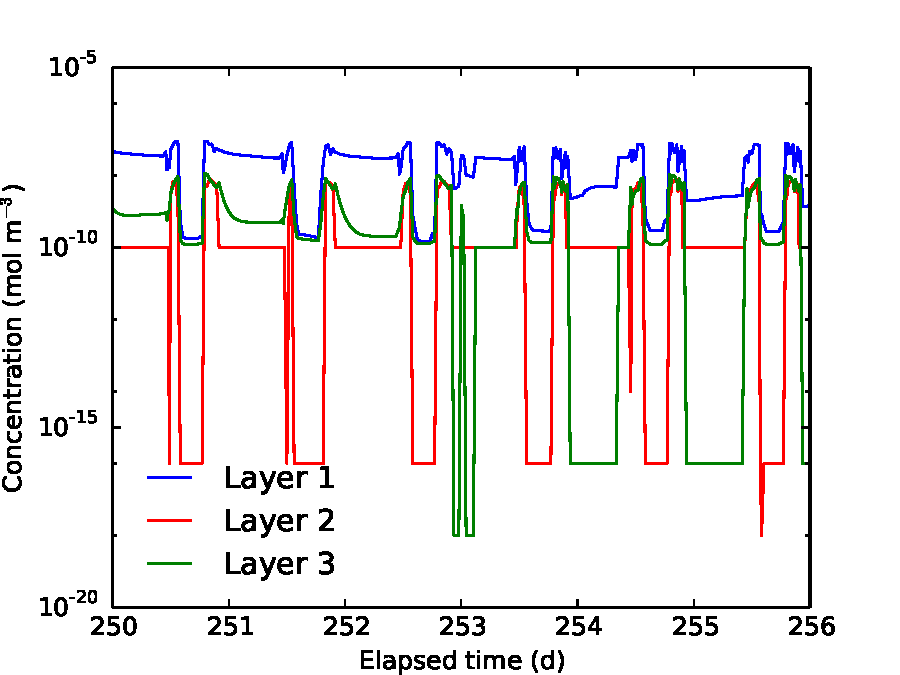
\includegraphics[width=0.5\textwidth]{../figs/fig15/caxn2o.pdf}
\caption{Diagnostic \chem{N_2O} concentration (\chem{N_2Od} from nitrification
associated with net nitrogen mineralization Reaction \ref{rxn:nitr2n2o} and
rate Eq. \ref{eq:nitr2n2odecomp}) in the spin-up simulation for the BR-Cax site
with $k_\text{m} = 10^{-6}$ \unit{mol\,m^{-3}}. The concentration is reset to
10$^{-10}$ at the beginning of each CLM half hour time step. Scaling back
update in each iteration is used to enforce nonnegativity.}
\label{fig:caxn2o}
\end{figure}

%\begin{figure}[t]
%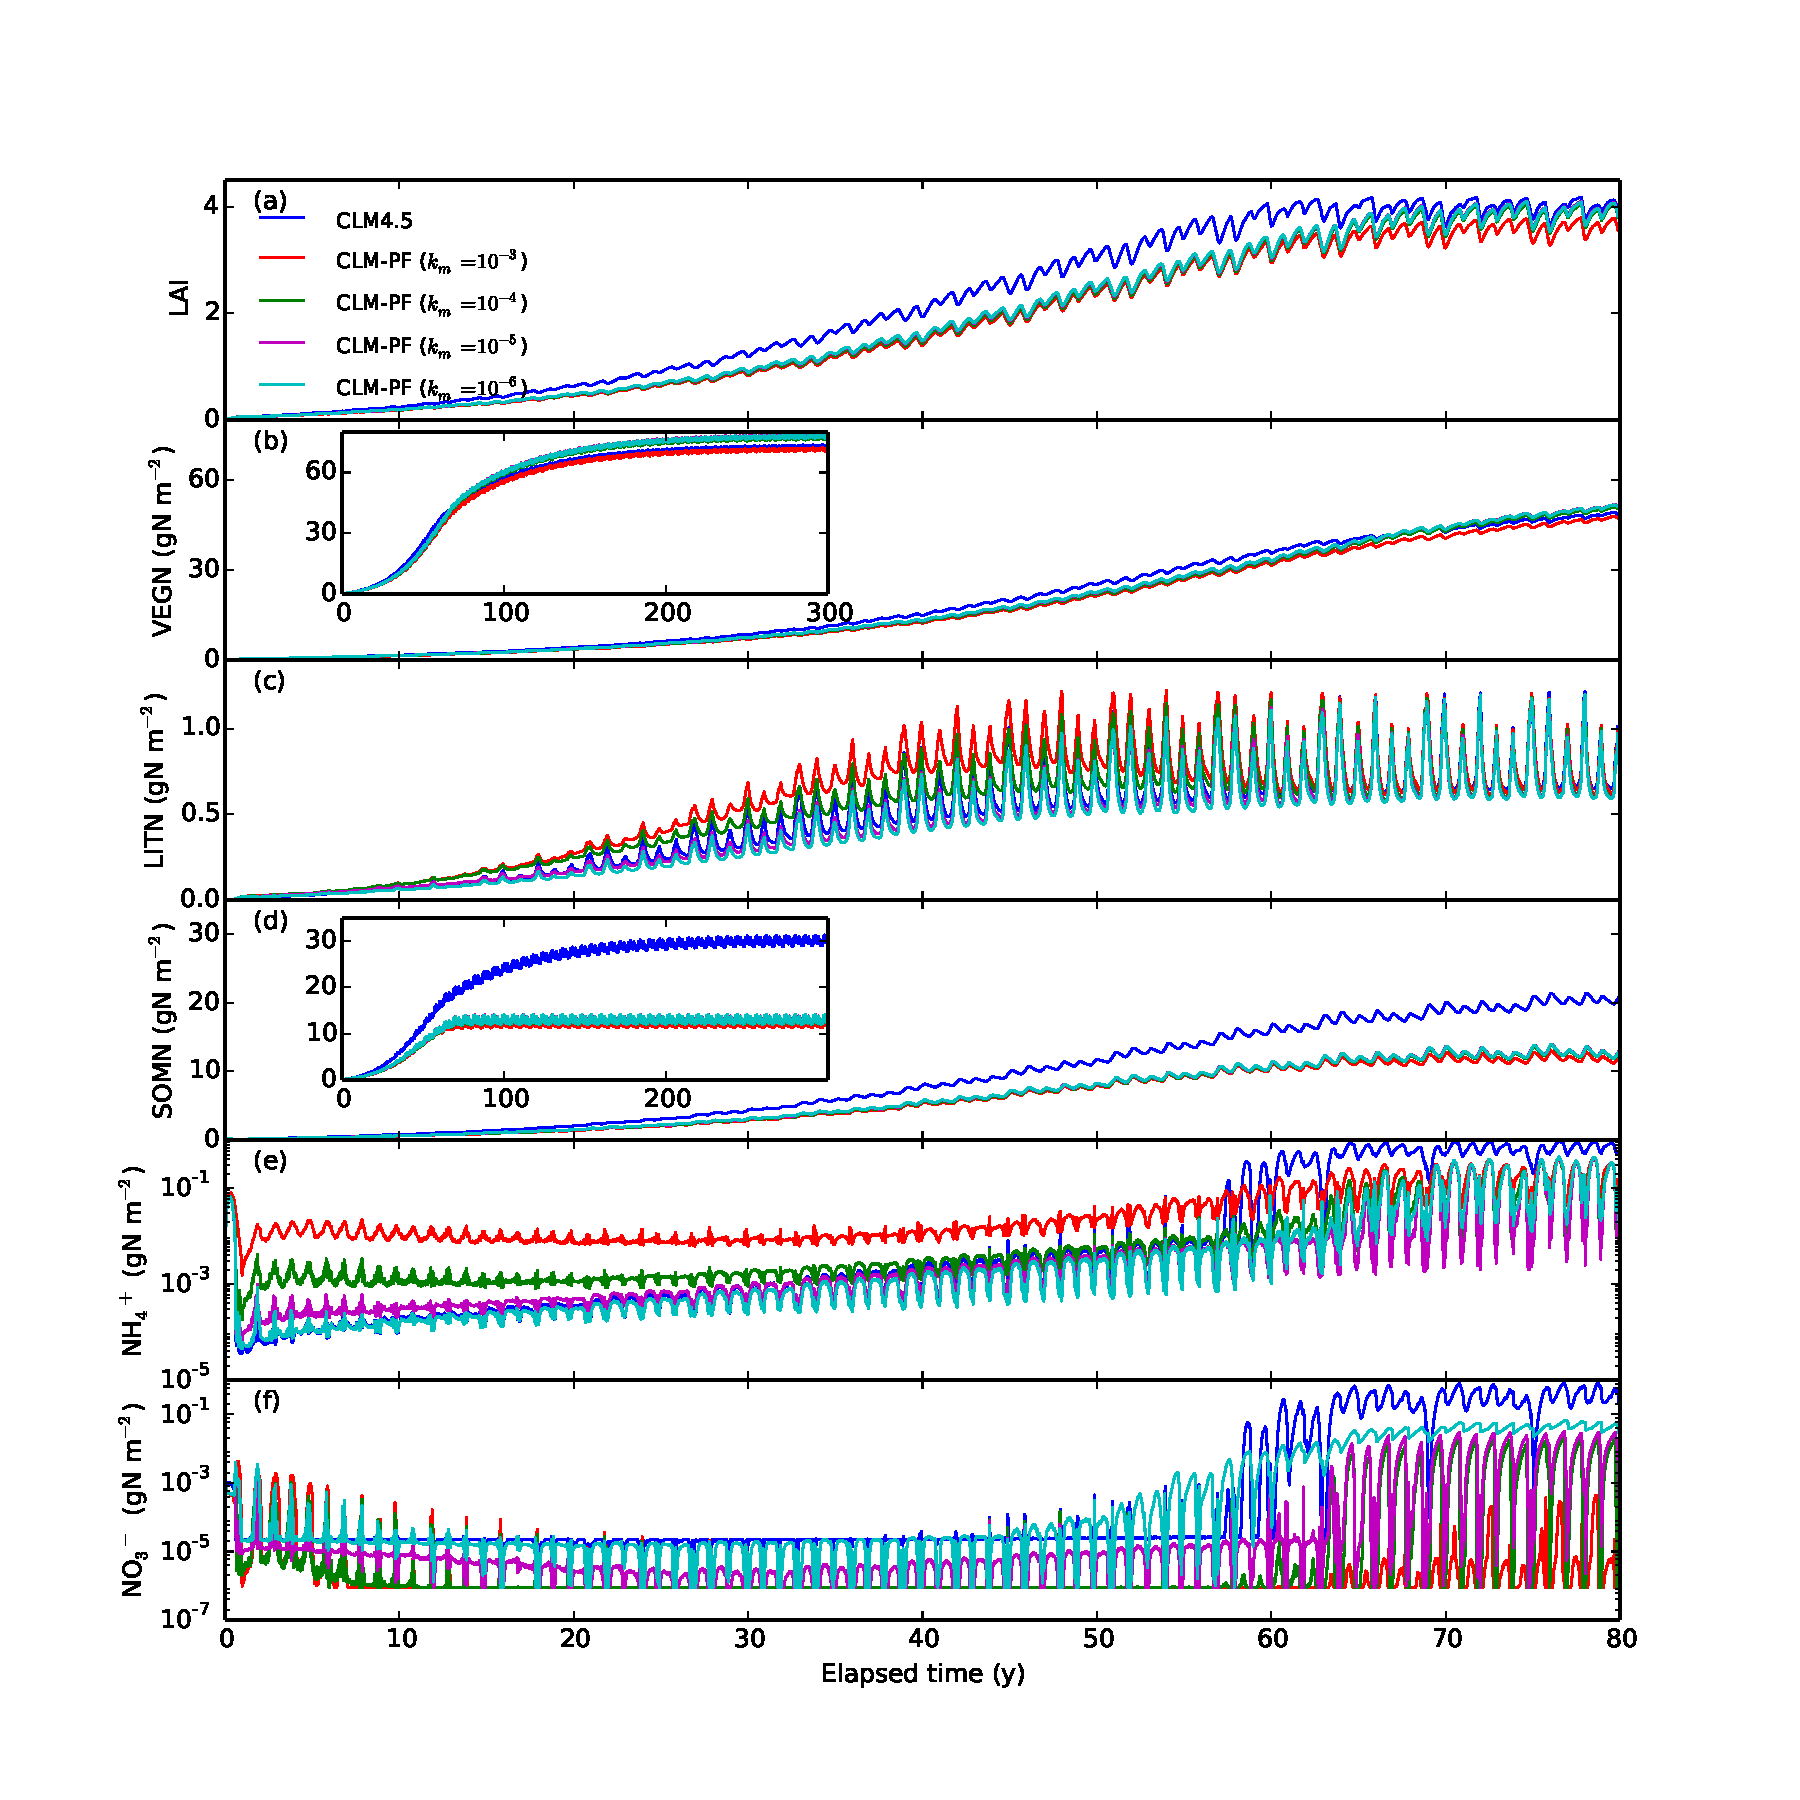
\includegraphics[width=1.0\textwidth]{../figs/fig16/cax300ycl.pdf}
%\caption{Calculated LAI and nitrogen distribution among vegetation, litter,
%SOM, \chem{NH_4^+}, and \chem{NO_3^-} pools in spin-up simulations for BR-Cax
%site using the CLM demand based competition for consumption downregulation, and
%log transformation to enforce nonnegativity. }
%\label{fig:cax300ycl}
%\end{figure}

%\input{tabls}


\clearpage

\begin{table}[t]
\caption{Wall time (hour) for spin-up simulation at the arctic, temperate, and tropical sites on OIC}
\label{tab:computingtime}
\begin{tabular}{rrrrrrrrr}
\tophline
Site & CLM  & SU ($10^{-3}$) & SU ($10^{-6}$) & SU ($10^{-9}$) & LT ($10^{-3}$) & LT ($10^{-6}$) & LT ($10^{-9}$) & LT ($10^{-12}$)\\
DC\\
US-Brw & 18.1 & 24.8 & 25.5 & 29.2 & 38.5 & 40.8 & 47.0 & 49.5 \\
US-Pit & 11.7 & 17.1 & 14.8 & 14.9 & 30.0 & 37.5 & 40.2 & 43.1 \\
BR-Cax & 10.9 & 16.2 & 18.6 & 18.0 & 40.2 & 40.5 & 45.7 & 52.0 \\
\middlehline
DR\\
US-Brw & 18.1 & 21.5 & 21.5 &      & 35.8 & 35.9 & \\
US-Pit & 11.7 & 14.1 & 14.1 &      & 26.9 & 26.7 & \\
BR-Cax & 10.9 & 16.4 & 16.4 &      & 42.2 & 41.6 & \\
\bottomhline
\end{tabular}
\belowtable{SU = scaling update, LT = log transformation, $10^{-3}$, $10^{-6}$, and $10^{-9}$ are $k_\text{m}$, DC and DR = downregulating consumption as a function of concentration and rate, OIC = ORNL Institutional Cluster (Phase5), US-Brw simulation duration = 500 year and US-Pit and BR-Cax simulation duration = 300 year. For the last column LT ($10^{-12}$), MAX\_CUT is increased from default 16 to 50.} % Table Footnotes
\end{table}

%\begin{table}[t]
%\caption{CLM-PFLOTRAN simulation termination before conclusion using scaling back update in iteration}
%\label{tab:stability}
%\begin{tabular}{rrrrrrr}
%\tophline
%Site & $k_\text{m}$ & year & species & concentration & update & layer\\
%\middlehline
%STOL = $10^{-8}$\\
%US-Brw & 10$^{-12}$ & 346.66 & \chem{NO_3^-} & $1.26\times 10^{-26}$ & $8.20\times10^{-15}$ & 4 \\
%US-Pit & 10$^{-12}$ & 3.56 & \chem{NO_3^-} & $2.67\times 10^{-26}$ & $2.49\times10^{-14}$ & 8 \\
%BR-Cax & 10$^{-12}$ & 3.18 & \chem{NO_3^-} & $2.54\times 10^{-26}$ & $5.72\times10^{-14}$ & 8 \\
%\middlehline
%STOL = $10^{-12}$\\
%US-Brw & 10$^{-6}$ & 41.78 & DeniN & 10$^{-20}$ & $2.31\times10^{-10}$ & 2 \\
%US-Brw & 10$^{-9}$ & 5.56 & PlantN  & $6.68\times 10^{-18}$ & $8.12\times10^{-8}$ & 2 \\
%US-PIT & 10$^{-3}$ & 7.81 & N$_2$Od & 10$^{-20}$ & $1.74\times10^{-9}$ & 1 \\
%US-PIT & 10$^{-6}$ & 2.40 & PlantN  & 10$^{-18}$ & $2.30\times10^{-6}$ & 1 \\
%BR-Cax & 10$^{-3}$ & 1.59 & N$_2$Od & 10$^{-20}$ & $1.66\times10^{-10}$ & 1 \\
%BR-Cax & 10$^{-6}$ & 0.64 & N$_2$Od & 10$^{-20}$ & $1.91\times10^{-10}$ & 2 \\
%BR-Cax & 10$^{-9}$ & 0.59 & PlantN  & 10$^{-18}$ & $4.92\times10^{-8}$ & 2 \\
%\bottomhline
%\end{tabular}
%\belowtable{} % Table Footnotes
%\end{table}

\clearpage

%% Since the Copernicus LaTeX package includes the BibTeX style file copernicus.bst,
%% authors experienced with BibTeX only have to include the following two lines:
%%
%% \bibliographystyle{copernicus}
%% \bibliography{example.bib}
%%
%% URLs and DOIs can be entered in your BibTeX file as:
%%
%% URL = {http://www.xyz.org/~jones/idx_g.htm}
%% DOI = {10.5194/xyz}


%% LITERATURE CITATIONS
%%
%% command                        & example result
%% \citet{jones90}|               & Jones et al. (1990)
%% \citep{jones90}|               & (Jones et al., 1990)
%% \citep{jones90,jones93}|       & (Jones et al., 1990, 1993)
%% \citep[p.~32]{jones90}|        & (Jones et al., 1990, p.~32)
%% \citep[e.g.,][]{jones90}|      & (e.g., Jones et al., 1990)
%% \citep[e.g.,][p.~32]{jones90}| & (e.g., Jones et al., 1990, p.~32)
%% \citeauthor{jones90}|          & Jones et al.
%% \citeyear{jones90}|            & 1990



%% FIGURES

%% ONE-COLUMN FIGURES

%%f
%\begin{figure}[t]
%\includegraphics[width=8.3cm]{FILE NAME}
%\caption{TEXT}
%\end{figure}
%
%%% TWO-COLUMN FIGURES
%
%%f
%\begin{figure*}[t]
%\includegraphics[width=12cm]{FILE NAME}
%\caption{TEXT}
%\end{figure*}
%
%
%%% TABLES
%%%
%%% The different columns must be seperated with a & command and should
%%% end with \\ to identify the column brake.
%
%%% ONE-COLUMN TABLE
%
%%t
%\begin{table}[t]
%\caption{TEXT}
%\begin{tabular}{column = lcr}
%\tophline
%
%\middlehline
%
%\bottomhline
%\end{tabular}
%\belowtable{} % Table Footnotes
%\end{table}
%
%%% TWO-COLUMN TABLE
%
%%t
%\begin{table*}[t]
%\caption{TEXT}
%\begin{tabular}{column = lcr}
%\tophline
%
%\middlehline
%
%\bottomhline
%\end{tabular}
%\belowtable{} % Table Footnotes
%\end{table*}
%
%
%%% NUMBERING OF FIGURES AND TABLES
%%%
%%% If figures and tables must be numbered 1a, 1b, etc. the following command
%%% should be inserted before the begin{} command.
%
%\addtocounter{figure}{-1}\renewcommand{\thefigure}{\arabic{figure}a}
%
%
%%% MATHEMATICAL EXPRESSIONS
%
%%% All papers typeset by Copernicus Publications follow the math typesetting regulations
%%% given by the IUPAC Green Book (IUPAC: Quantities, Units and Symbols in Physical Chemistry,
%%% 2nd Edn., Blackwell Science, available at: http://old.iupac.org/publications/books/gbook/green_book_2ed.pdf, 1993).
%%%
%%% Physical quantities/variables are typeset in italic font (t for time, T for Temperature)
%%% Indices which are not defined are typeset in italic font (x, y, z, a, b, c)
%%% Items/objects which are defined are typeset in roman font (Car A, Car B)
%%% Descriptions/specifications which are defined by itself are typeset in roman font (abs, rel, ref, tot, net, ice)
%%% Abbreviations from 2 letters are typeset in roman font (RH, LAI)
%%% Vectors are identified in bold italic font using \vec{x}
%%% Matrices are identified in bold roman font
%%% Multiplication signs are typeset using the LaTeX commands \times (for vector products, grids, and exponential notations) or \cdot
%%% The character * should not be applied as mutliplication sign
%
%
%%% EQUATIONS
%
%%% Single-row equation
%
%\begin{equation}
%
%\end{equation}
%
%%% Multiline equation
%
%\begin{align}
%& 3 + 5 = 8\\
%& 3 + 5 = 8\\
%& 3 + 5 = 8
%\end{align}
%
%
%%% MATRICES
%
%\begin{matrix}
%x & y & z\\
%x & y & z\\
%x & y & z\\
%\end{matrix}
%
%
%%% ALGORITHM
%
%\begin{algorithm}
%\caption{}
%\label{a1}
%\begin{algorithmic}
%
%\end{algorithmic}
%\end{algorithm}
%
%
%%% CHEMICAL FORMULAS AND REACTIONS
%
%%% For formulas embedded in the text, please use \chem{}
%
%%% The reaction environment creates labels including the letter R, i.e. (R1), (R2), etc.
%
%\begin{reaction}
%%% \rightarrow should be used for normal (one-way) chemical reactions
%%% \rightleftharpoons should be used for equilibria
%%% \leftrightarrow should be used for resonance structures
%\end{reaction}
%
%
%%% PHYSICAL UNITS
%%%
%%% Please use \unit{} and apply the exponential notation

%\input{appendix}

\appendix

\section{CLM biogeochemical reactions and rates}
\label{sec:clmbgc}
\subsection{CLM-CN decomposition}
\label{section:bgc}

The CLM-CN decomposition cascade consists of three litter pools with variable
CN ratios, four soil organic matter (SOM) pools with constant CN ratios, and
seven reactions (Fig. \ref{fig:conceptualmodel}A). The reaction can be
described by
\begin{reaction}
\chem{CN_u} \rightarrow (1 - f) \chem{CN_d} + f \chem{CO_2} + n \chem{N},
\label{rxn:decomp}
\end{reaction}
with \chem{CN_u} and \chem{CN_d} as the upstream and downstream pool (molecular
formula, for 1 mol upstream and downstream pool, there is u and d mol N),
\chem{N} as either \chem{NH_4^+} or \chem{NO_3^-}, \textit{f} as the
respiration fraction, and \textit{n} = u $-$ (1 $-$ \textit{f})d. The rate is
\begin{equation}
\frac{d [\chem{CN_u}]}{d t} = - k_\text{d} f_\text{T} f_\text{w} [\chem{CN_u}],
\label{eq:decomprate}
\end{equation}
with $\textit{k}_\text{d}$ as the rate coefficient and $\textit{f}_\text{T}$
and $\textit{f}_\text{w}$ as the temperature and moisture response functions,
\begin{equation}
f_T = Q_{10}^{(T - 25)/10}, 
\end{equation}
and
\begin{equation}
f_w = \ln(\psi)Q_{10}^{(T - 25)/10}, 
\end{equation}
With a constant CN ratio, the decomposition reactions for the four SOM pools are 
\begin{reaction}
\chem{SOM1} \rightarrow 0.72 \chem{SOM2} + 0.28 \chem{CO_2} + 0.02 \chem{N},
\label{rxn:som1}
\end{reaction}
\begin{reaction}
\chem{SOM2} \rightarrow 0.54 \chem{SOM3} + 0.46 \chem{CO_2} + 0.025143 \chem{N},
\label{rxn:som2}
\end{reaction}
\begin{reaction}
\chem{SOM3} \rightarrow 0.45 \chem{SOM4} + 0.55 \chem{CO_2} + 0.047143 \chem{N},
\label{rxn:som3}
\end{reaction}
and
\begin{reaction}
\chem{SOM4} \rightarrow \chem{CO_2} + 0.085714 \chem{N}.
\label{rxn:som4}
\end{reaction}
The exact stoichiometric coefficients are calculated in the code using values
for respiration factor, CN ratio, and molecular weight specified in the input
file.

CLM4.5 has an option to separate \chem{N} into \chem{NH_4^+} and \chem{NO_3^-}.
The \chem{N} mineralization product is \chem{NH_4^+}.
% see CNNStateUpdate1Mod.F90 line 359-391. 

As the CN ratio is variable for the three litter pools, litter N pools need to
be tracked such that reaction (\ref{rxn:decomp}) becomes
\begin{reaction}
\chem{LitC} + u \chem{LitN} \rightarrow (1 - f) \chem{CN_d} + f \chem{CO_2} + n \chem{N}, 
\label{rxn:lit}
\end{reaction}
with $\textit{u}$ = [LitN]/[LitC]. The three litter decomposition reactions are
\begin{reaction}
\chem{Lit1C} + u_1 \chem{Lit1N} \rightarrow 0.41 \chem{SOM1} + 0.39 \chem{CO_2} + (u_1 - 0.029286) \chem{N},
\label{rxn:lit1}
\end{reaction}
\begin{reaction}
\chem{Lit2C} + u_2 \chem{Lit2N} \rightarrow 0.45 \chem{SOM2} + 0.55 \chem{CO_2} + (u_2 - 0.032143) \chem{N},
\label{rxn:lit2}
\end{reaction}
and
\begin{reaction}
\chem{Lit3C} + u_3 \chem{Lit3N} \rightarrow 0.71 \chem{SOM3} + 0.29 \chem{CO_2} + (u_3 - 0.060857) \chem{N}.
\label{rxn:lit3}
\end{reaction}
As the CN ratio of the litter pools is generally  high, $u_1$, $u_2$, and $u_3$
are usually small, and $n$ in these reactions (e.g., $n_1 = u_1 - 0.029286$ for
\chem{Lit1}) is normally negative. Namely, these reactions consume (immobilize)
\chem{N}, which can be \chem{NH_4^+}, \chem{NO_3^-}, or both. 

\subsection{Nitrification}
The nitrification reaction to produce \chem{NO_3^-} is 
\begin{reaction}
\chem{NH_4^+} + \cdots \rightarrow \chem{NO_3^-} + \cdots
\label{rxn:nitr2no3}
\end{reaction}
with $\cdots$ for additional reactants and products to balance the reaction. The
rate is (Dickinson et al., 2002) 
\begin{equation}
\frac{d [\chem{NH_4^+}]}{d t} = -\frac{d
[\chem{NO_3^-]}}{d t} = -k_\text{n} f_\text{T} f_\text{w}
[\chem{NH_4^+}].
\label{eq:nitr2no3}
\end{equation}
The nitrification reaction to produce $\chem{N_2O}$ is
\begin{reaction}
\chem{NH_4^+} + \cdots \rightarrow 0.5 \chem{N_2O} + \cdots,
\label{rxn:nitr2n2o}
\end{reaction}
with one component related to decomposition as %when
%$\chem{NH_4^+}$ is low ( < 3 $\mu \text{gN g}^{-1}$) as 
\begin{equation}
\frac{d [\chem{NH_4^+}]}{d t} = -2\frac{d
[\chem{N_2O}]}{d t} = -f_\text{nm} f_\text{T} f_\text{w}
f_\text{pH}\max(R_\text{nm},0)
\label{eq:nitr2n2odecomp}
\end{equation}
with $f_\text{nm}$ as a fraction \citep{Parton1996} and $R_\text{nm}$ as the
net \chem{N} mineralization rate,  
\begin{equation}
R_\text{nm}=\sum_{i} n_iR_i,
\label{eq:netnmin}
\end{equation}
where $R_i$ denotes the rate of reaction (\ref{rxn:som1}, \ref{rxn:som2},
\ref{rxn:som3}, \ref{rxn:som4}, \ref{rxn:lit1}, \ref{rxn:lit2},
\ref{rxn:lit3}).
The second component is \citep{Parton1996} %relates to excessive \chem{NH_4^+}
%(> 3 $\mu$gN g$^{-1}$) 
\begin{equation} 
\frac{d [\chem{NH_4^+}]}{d t} = -2\frac{d
[\chem{N_2O}]}{d t} = -k_\text{n2o} f_\text{T} f_\text{w}
f_\text{pH}(1-e^{-0.0105[\chem{NH_4^+}]}).
\label{eq:nitr2n2oexess}
\end{equation}
Ignoring the high-order terms and moving the unit conversion factor into
$k_\text{n2o}$, it can be simplified as a first-order
rate as
\begin{equation} 
\frac{d [\chem{NH_4^+}]}{d t} = -2\frac{d
[\chem{N_2O}]}{d t} = -k_\text{n2o} f_\text{T} f_\text{w}
f_\text{pH}[\chem{NH_4^+}].
\label{eq:nitr2n2oexesssimple}
\end{equation}

\subsection{Denitrification} 
The denitrification reaction is
\begin{reaction}
\chem{NO_3^-} + \cdots \rightarrow 0.5 \chem{N_2} + \cdots
\label{rxn:deni}
\end{reaction}
with rate \citep{Dickinson2002} 
\begin{equation} 
\frac{d [\chem{NO_3^-}]}{d t} = -2\frac{d
[\chem{N_2}]}{d t} = -k_\text{deni} f_\text{T} f_\text{w}
f_\text{pH}[\chem{NO_3^-}].
\label{eq:deni}
\end{equation}

\subsection{Plant nitrogen uptake}
The plant nitrogen uptake reaction can be written as
\begin{reaction}
\chem{NH_4^+} + \cdots \rightarrow \chem{PlantA} + \cdots
\label{rxn:plantatake}
\end{reaction}
and
\begin{reaction}
\chem{NO_3^-} + \cdots \rightarrow \chem{PlantN} + \cdots.
\label{rxn:plantntake}
\end{reaction}
The rate is specified by CLM (plant nitrogen demand) and assumed to be
constant in each half-hour time step. 

\subsection{Demand-based competition and distributing nitrogen demand between \chem{NH_4^+} and \chem{NO_3^-}}
\label{sec:demandbasedcompetition}
Denote $R_{d,p}$, $R_{d,i}$, $R_{d,nitr}$, $R_{d,deni}$ as the potential plant,
immobilization, nitrification, and denitrification demand (rate);
$R_{a,tot}=R_{d,p}+R_{d,i}+R_{d,nitr}$ as the total \chem{NH_4^+} demand; and
$R_{n,tot}$ as the total \chem{NO_3^-} demand. CLM uses a demand-based
competition approach to split the available sources in proportion to the demand
rates to meet the demands \citep{Oleson2013,Thornton2005}. Specifically, for
each time step, if $R_{a,tot}\Delta t \leq [\chem{NH_4^+}]$, the uptakes are
equal to potential demands, and $R_{n,tot}$ = 0; otherwise, the uptakes for
\chem{NH_4^+} are [\chem{NH_4^+}]$R_{d,p}/R_{a,tot}\Delta t$,
[\chem{NH_4^+}]$R_{d,i}/R_{a,tot}\Delta t$, and
[\chem{NH_4^+}]$R_{d,nitr}/R_{a,tot}\Delta t$ for plants, immobilization, and
nitrification, respectively; $R_{n,tot}=R_{a,tot}-[\chem{NH_4^+}]/\Delta t +
R_{d,deni}$. If $R_{n,tot}\Delta t < [\chem{NO_3^-}]$, all of the remaining
demand $R_{n,tot}$ is met with available \chem{NO_3^-}. Otherwise, available
\chem{NO_3^-} is split to meet the remaining plant, immobilization, and
denitrification demands in proportion to their rates. 

\section{Downregulation with cutoff}
\label{sec:cutoff}
An alternative to using a residual concentration (Eq. \ref{eq:decomprateresidual}) is to
introduce a cutoff, e.g., Eq. (\ref{eq:decomprate}) becomes
\begin{equation}
\frac{d [\chem{CN_u}]}{d t} = -k_\text{d} f_\text{T} f_\text{w}
[\chem{CN_u}] f([\chem{CN_u}]),
\end{equation}
with $f([\chem{CN_u}]) = 1$ when [\chem{CN_u}]$\geq$[\chem{CN_u}]$_\text{r}$,
and 0 otherwise. It is simple but does not prevent [\chem{CN_u}] from getting
below [\chem{CN_u}]$_\text{r}$ or 0 in theory. In addition, it introduces a
discontinuity. A polynomial function can be used to smooth the cutoff 
\begin{equation}
f([\chem{CN_u} ])=1-\left[1-\left(\frac{[\chem{CN_u}]-[\chem{CN_u}
]_\text{r}}{\chem{CN_u} ]_1-[\chem{CN_u} ]_\text{r}}\right)^2 \right]^2.
\label{eq:polycutoff}
\end{equation}
This function varies from 0 at [\chem{CN_u}]$_\text{r}$ to 1 at
[\chem{CN_u}]$_1$, with zero derivatives at both points. While not implying a
nonphysical reverse reaction as Eq. (\ref{eq:decomprateresidual}), 
\begin{equation}
\frac{d f([\chem{CN_u} ])}{d[\chem{CN_u}]}=4 \frac{[\chem{CN_u}] -
[\chem{CN_u}]_\text{r}}{\left([\chem{CN_u}]_1 - [\chem{CN_u}]_\text{r} \right)^2}
\left[1-\left(\frac{[\chem{CN_u}]-[\chem{CN_u} ]_\text{r}}{\chem{CN_u}
]_1-[\chem{CN_u} ]_\text{r}}\right)^2 \right].
\label{eq:polycutoffderiv}
\end{equation}
Depending on $[\chem{CN_u}]_1-[\chem{CN_u}]_\text{r}$, this cutoff does
introduce a large derivative change during the transition:
$df([\chem{CN_u}])/d[\chem{CN_u}]$ varies from 0 to ~10$^8$ for
[\chem{CN_u}]$_\text{r}$=10$^{-10}$  and [\chem{CN_u}]$_1$=10$^{-8}$ (Fig.
\ref{fig:cutoff}). The maximum increases at about the same order of magnitude
as the decrease of [\chem{CN_u}]$_r$ and [\chem{CN_u}]$_1$. Even though
smoothed, the cutoff is still a sharp change. The smaller the cutoff
concentrations, the sharper the transitions. Marching through a steep
transition in time usually involves small time steps.
\begin{figure}[h]
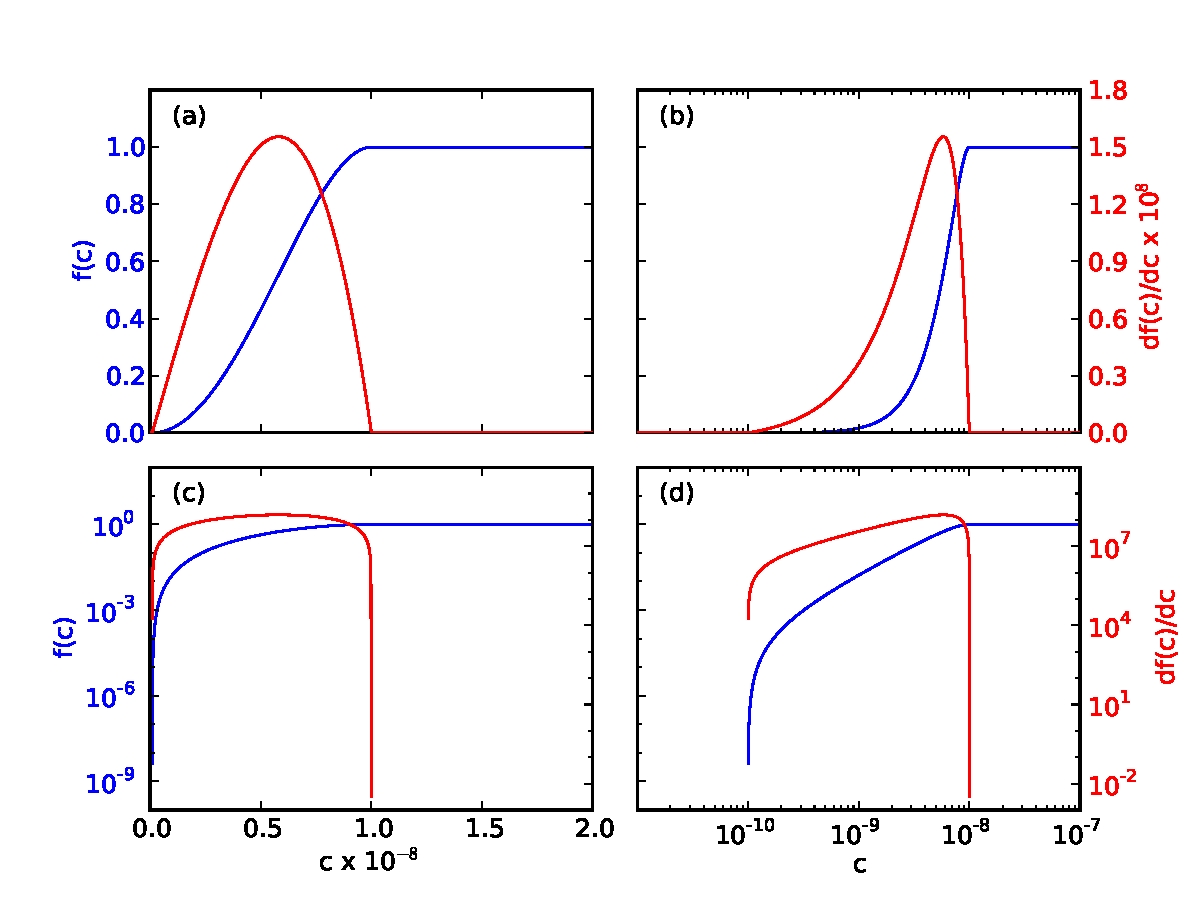
\includegraphics[width=1.0\textwidth]{../figs/fig02/fig02cutoff.pdf}
\caption{Smoothed cutoff function (Eq. \ref{eq:polycutoff}) and derivative (Eq.
\ref{eq:polycutoffderiv}). The y axis is in log in (c) and (d), while the x
axis is in log in (b) and (d). Even though smoothed, the cutoff is a steep
transition. The derivative varies by orders of magnitude in a small
concentration range and requires small time step size to march through.}
\label{fig:cutoff}
\end{figure}

\section{Downregulation of consumption as a function of rates}    %% Appendix A
\label{sec:drimpl}
The contribution of $n$ reactions to the rate component in the residual and
Jacobian for species $i$ are
\begin{equation}
\mathbf{R}(i)=\sum_{j=1}^n \nu_{ij} R_j,
\end{equation}
and
\begin{equation}
\mathbf{J}(i,k)=\frac{\partial \mathbf{R}(i)}{\partial \mathbf{C}(k)} =
\sum_{j=1}^n \frac{\partial (\nu_{ij} R_j)}{\partial \mathbf{C}(k)},
\end{equation}
with $\mathbf{C}$ as the concentration vector, $\mathbf{R}$ as the rate vector,
$\mathbf{J}$ as the component of Jacobian matrix (m by m) that is associated
with $\mathbf{R}$, $\nu_{ij}$ as stoichiometric coefficient of species $i$ in
reaction $j$ ($\sum_{i=1}^m \nu_{ij} \mathbf{C}(i) = 0$), and $R_j$ as the rate of
reaction $j$, a function of the activities (concentration) of the reactants,
products, and environmental variables (moisture, temperature, pH, redox, etc.).

\subsection{Downregulation of consumption for one species}
Depending on whether a species a (e.g., \chem{NH_4^+}) is a reactant
($\nu_{aj}$ > 0) or a product ($\nu_{aj}$ < 0), we divide the $n$ reactions into a
demand (subscript $da$ for demand $a$) and a supply (subscript $sa$ for supply
$a$) group:
\begin{equation}
R_{da}=\sum_{j=1}^{n_{da}} \nu_{da,aj} R_{da,j},
\end{equation}
and
\begin{equation}
R_{sa}=\sum_{j=1}^{n_{sa}} \nu_{sa,aj} R_{sa,j},
\end{equation}
with $n_{da}$ as the number of reactions that consume species $a$,
$\nu_{da,aj}$ as the stoichiometric coefficient of species $i$ in $a$ consuming
reaction $j$, $n_{sa}$ as the number of reactions that produce species $a$,
$\nu_{sa,ij}$ as the stoichiometric coefficient of species $i$ in a producing
reaction $j$, $R_{da}$ as $a$ consumption (demand) rate (mol s$^{-1}$,
negative), and $R_{sa}$ as $a$ production (supply) rate (mol s$^{-1}$,
positive). Therefore, 
\begin{equation}
\mathbf{R}(i) = \sum_{j=1}^{n_{sa}} \nu_{sa,aj} R_{sa,j} + \sum_{j=1}^{n_{da}}
\nu_{da,aj} R_{da,j}=\mathbf{R}_{sa} (i)+\mathbf{R}_{da} (i),
\end{equation}
and
\begin{equation}
\mathbf{J}(i,k)=\frac{\partial \mathbf{R}(i)}{\partial \mathbf{C}(k)}
=\sum_{j=1}^n \frac{\partial (\nu_{ij}R_j)}{\partial \mathbf{C}(k)} =
\sum_{j=1}^{n_{sa}} \frac{\partial (\nu_{sa,ij}R_{sa,j})}{\partial
\mathbf{C}(k)} + \sum_{j=1}^{n_{da}} \frac{\partial
(\nu_{da,ij}R_{da,j})}{\partial \mathbf{C}(k)} =
\mathbf{J}_{sa}+\mathbf{J}_{da}.
\end{equation}
%\begin{equation}
%\mathbf{J}=\mathbf{J}_{sa}+\mathbf{J}_{da}
%\end{equation}

Define a downregulation factor  
\begin{equation}
d_a=\min\left(1, -\frac{R_{sa} \Delta t + \left[\mathbf{C}(a)-\epsilon\right]
V} {R_{da} \Delta t}\right)=\min\left(1, -\frac{s_a}{D_a}\right),
\end{equation} 
with $V$ as the bulk volume or volume of liquid water of the grid cell for
species with concentration unit \chem{mol\,m^{-3}} or \chem{M}. After
downregulation,
\begin{equation}
\mathbf{R}_a=\mathbf{R}_{sa}+d_a \mathbf{R}_{da},
\end{equation}
\begin{equation}
\mathbf{J}_a (i,k)=\frac{\partial \mathbf{R}_a(i)}{\partial \mathbf{C}(k)}
=\mathbf{J}_{sa} (i,k)+d_a \mathbf{J}_{da} (i,k)+\mathbf{R}_{da} (i)
\frac{\partial d_a}{\partial \mathbf{C}(k)}, 
\end{equation}
\begin{equation}
\frac{\partial d_a}{\partial \mathbf{C}(k)} =-\left(\frac{\partial
s_a}{\partial \mathbf{C}(k)} D_a - s_a \frac{\partial D_a}{\partial
\mathbf{C}(k)}\right)D_a^{-2}, 
\end{equation}
\begin{equation}
\frac{\partial s_a}{\partial \mathbf{C}(a)} =\sum_{j=1}^{n_{sa}}
\frac{\partial (\nu_{sa,aj}R_{sa,j})}{\partial \mathbf{C}(a)} \Delta t + V, 
\end{equation}
\begin{equation}
\frac{\partial s_a}{\partial \mathbf{C}(k)} =\sum_{j=1}^{n_{sa}}
\frac{\partial (\nu_{sa,kj}R_{sa,j})}{\partial \mathbf{C}(k)} \Delta t, 
\end{equation}
\begin{equation}
\frac{\partial D_a}{\partial \mathbf{C}(k)} =\sum_{j=1}^{n_{da}}
\frac{\partial (\nu_{da,kj}R_{da,j})}{\partial \mathbf{C}(k)} \Delta t, 
\end{equation}
Implementation in PFLOTRAN involves 1) adding variables $\mathbf{R}_{sa}$,
$\mathbf{R}_{da}$, and $\mathbf{J}_a$, 2) accumulating the values in each
reaction rate formula, and 3) conducting downregulation and adding the
contribution to the global residual vector and Jacobian matrix. 

\subsection{Downregulation of consumption for a second species}
In addition to species $a$ (e.g., \chem{NH_4^+}), we want to downregulate
another species $l$, for example, \chem{NO_3^-}. The treatment is the same
except for the reactions that consume species $a$ and produce species $l$.
Suppose we have a nitrification reaction (\ref{rxn:nitr2no3}) with rate
$R_{al}$, and $R_{al}' = dR_{al}/d[\chem{NH_4^+}]$. The rate and derivative are
added in demand rate and derivative for \chem{NH_4^+} ($\mathbf{R}_{sa}$,
$\mathbf{R}_{da}$, $\mathbf{J}_{sa}$, $\mathbf{J}_{da}$), not in the sink rate
and derivative for \chem{NO_3^-} ($\mathbf{R}_{sl}$,$\mathbf{R}_{dl}$,
$\mathbf{J}_{sl}$, $\mathbf{J}_{dl}$). Define a downregulation factor 
\begin{equation}
d_l=\min\left(1, -\frac{R_{sl} \Delta t + (\mathbf{C}(l)-\epsilon) V_w +
\underline{R_{al}d_a\Delta t}} {R_{dl} \Delta t}\right)=\min(1,
-\frac{s_l}{D_l}),
\end{equation}
\begin{equation}
\mathbf{R}_l=\mathbf{R}_{sl}+d_l \mathbf{R}_{dl},
\end{equation}
\begin{equation}
\mathbf{J}_l (i,k)=\frac{\partial \mathbf{R}_l(i)}{\partial \mathbf{C}(k)}
=\mathbf{J}_{sl} (i,k)+d_l \mathbf{J}_{dl} (i,k)+\mathbf{R}_{dl} (i)
\frac{\partial d_l}{\partial \mathbf{C}(k)}, 
\end{equation}
\begin{equation}
\frac{\partial d_l}{\partial \mathbf{C}(k)} =-\left(\frac{\partial
s_l}{\partial \mathbf{C}(k)} D_l - s_l \frac{\partial D_l}{\partial
\mathbf{C}(k)}\right)D_l^{-2}, 
\end{equation}
\begin{equation}
\frac{\partial s_l}{\partial \mathbf{C}(l)} =\sum_{j=1}^{n_{sl}}
\frac{\partial (\nu_{sl,lj}R_{sl,j})}{\partial \mathbf{C}(l)} \Delta t + V_w +
\underline{\frac{\partial (R_{al}d_a)}{\partial \mathbf{C}(l)}}, 
\end{equation}
\begin{equation}
\frac{\partial s_l}{\partial \mathbf{C}(k)} =\sum_{j=1}^{n_{sl}} \frac{\partial
(\nu_{sl,kj}R_{sl,j})}{\partial \mathbf{C}(k)} \Delta t +
\underline{\frac{\partial (R_{al}d_a)}{\partial \mathbf{C}(K)}}, 
\end{equation}
and
\begin{equation}
\frac{\partial D_a}{\partial \mathbf{C}(k)} =\sum_{j=1}^{n_{da}}
\frac{\partial (\nu_{da,kj}R_{da,j})}{\partial \mathbf{C}(k)} \Delta t. 
\end{equation}
In addition to variables $\mathbf{R}_{sl}$, $\mathbf{R}_{dl}$, and $\mathbf{J}_l$,
downregulating the second species requires two additional variables,
$R_{al}$, and $R_{al}'$. When accumulating the values in each reaction rate
formula, the production rate from the reaction that consumes the first species
has to be carefully treated as it is downregulated for the first species.
Conducting downregulation involves additional terms, as underlined in the
equations. Compared with the downregulation for the first species,
downregulating the second species that can be produced from the first species
with a simple $\chem{A}\rightarrow\chem{B}$ reaction becomes much more
complicated. If we add another reaction that consumes the second species to
produce the first species, this approach has to be modified. 

In general, many if not all species need to be downregulated. Extending this
approach involves adding many variables (vectors and matrices) to track the
consumption and production rates and their derivatives. The consumption and
production relationship among many species can be complicated, making
generalization of this approach challenging if not infeasible. 

\section{A semi-analytical solution for Monod equation}
\label{sec:monodsemi}
As an analytical solution is not available, discretizing Eq. (\ref{eq:ex1})
using the backward Euler method, it becomes
\begin{equation}
{[\chem{NH_4^+}]^{k+1}}^2+(k_\text{m} + R_a \Delta t - [\chem{NH_4^+}]^k)
[\chem{NH_4^+}]^{k+1} - k_\text{m} [\chem{NH_4^+}]^k = 0.
\end{equation}
The two roots are
\begin{equation}
[\chem{NH_4^+}]^{k+1}=0.5 \left[[\chem{NH_4^+}]^k - k_\text{m} - R_a \Delta t
\pm \sqrt{([\chem{NH_4^+}]^k - k_\text{m} - R_a\Delta t)^2 + 4
k_\text{m}[\chem{NH_4^+}]^k}\right].
\label{eq:monodsemi}
\end{equation}

\section{Matrix equation for example Test 2}
\begin{equation}
\left[
\begin{matrix}
\frac{1}{\Delta t} + J_{at} + J_{nitr} & 0 & 0 \\
-J_{at} & \frac{1}{\Delta t} & 0 \\
-J_{nitr} & 0 & \frac{1}{\Delta t} \\
\end{matrix}
\right]
\left(
\begin{matrix}
\delta [\chem{NH_4^+}]^{k+1,1} \\
\delta [\chem{PlantA}]^{k+1,1} \\
\delta [\chem{NO_3^-}]^{k+1,1} 
\end{matrix}
\right)
=
\left(
\begin{matrix}
R_{at} + R_{nitr} \\
-R_{at} \\
-R_{nitr} 
\end{matrix}
\right).
\label{eq:test2}
\end{equation}

\section{Matrix equation for example Test 3}
\label{sec:eqtest3}
\begin{equation}
\label{eq:complexjacobian}
\left[
\begin{matrix}
\frac{1}{\Delta t} + J_{at} + J_{nitr} & 0                  & 0                                   &0 & 0\\
-J_{at}                              & \frac{1}{\Delta t} & 0 &0 &0\\
-J_{nitr} + J_{nt,a}                 & 0                  & \frac{1}{\Delta t} + J_{nt} + J_{deni}&0 &0 \\
-J_{nt,a}                            & 0                  & -J_{nt,n}                             &1/\Delta t & 0 \\
 0                                   & 0                  & -0.5J_{deni}                             & 0 &1/\Delta t
\end{matrix}
\right]
\left(
\begin{matrix}
\delta [\chem{NH_4^+}]^{k+1,1} \\
\delta [\chem{PlantA}]^{k+1,1} \\
\delta [\chem{NO_3^-}]^{k+1,1} \\ 
\delta [\chem{PlantN}]^{k+1,1} \\
\delta [\chem{N_2}]^{k+1,1} 
\end{matrix}
\right)
=
\left(
\begin{matrix}
R_{at} + R_{nitr} \\
-R_{at} \\
-R_{nitr} + R_{nt} + R_{deni} \\
-R_{nt} \\
-0.5R_{deni}
\end{matrix}
\right).
\end{equation}

%\clearpage
\section{Supplemental figures}    %% Appendix A

\begin{figure}[h]
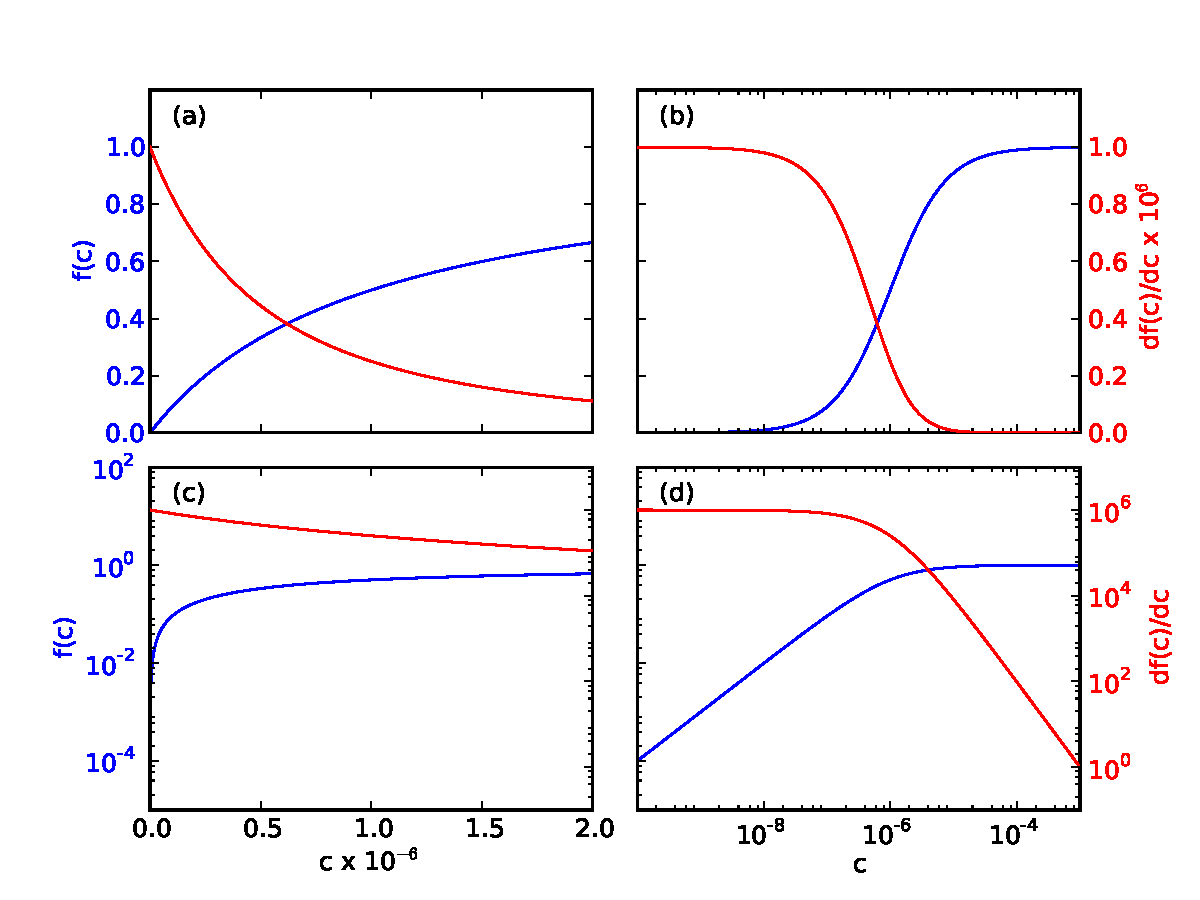
\includegraphics[width=1.0\textwidth]{../figs/fig03/fig03monod.pdf}
\caption{Monod substrate limiting function (Eq. \ref{eq:monod}) and derivative.
The y axis is in log in (c) and (d), while the x
axis is in log in (b) and (d). As the function switches from zero-order to
first-order, the derivative jumps six ($k_\text{m}^{-1}$) orders of magnitudes,
requiring small time step size to step through.}
\label{fig:monod}
\end{figure}


\begin{figure}[h]
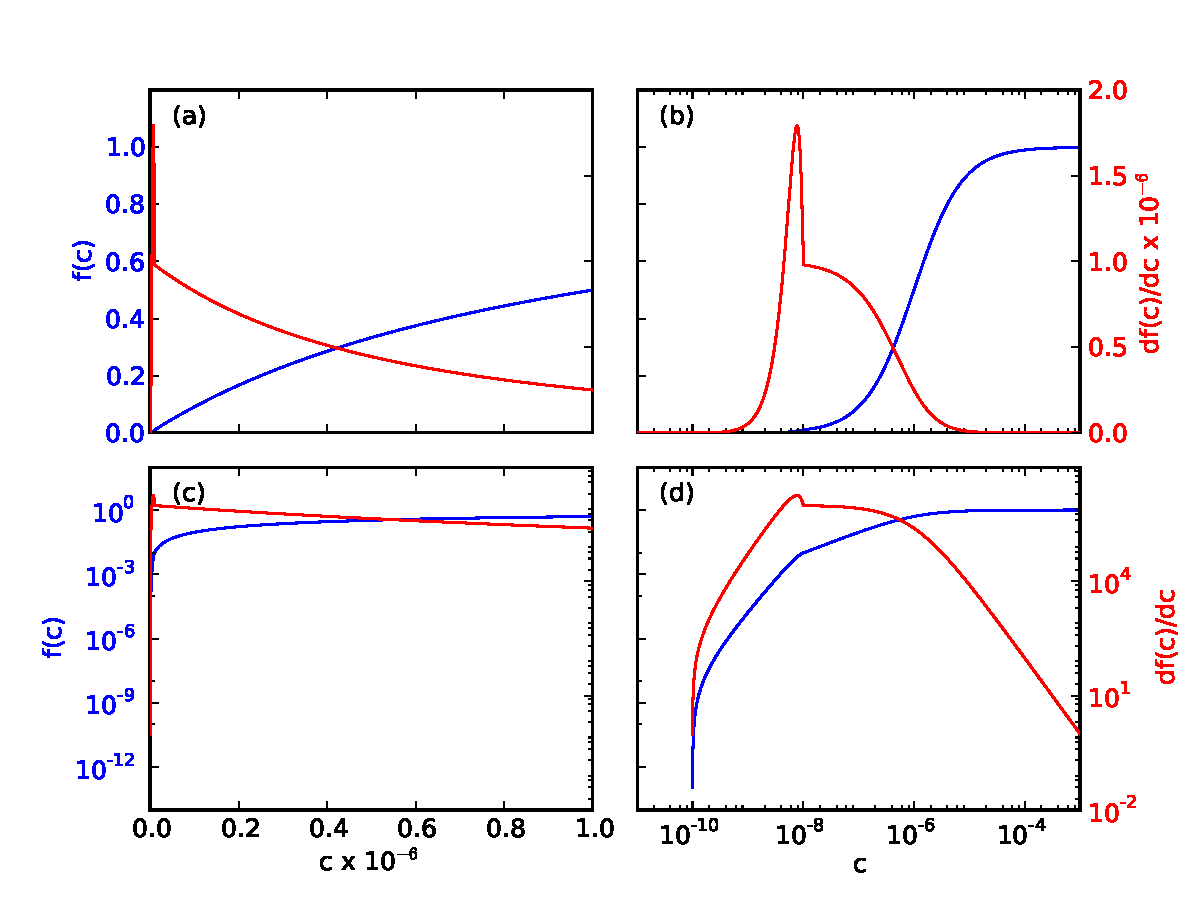
\includegraphics[width=1.0\textwidth]{../figs/fig04/fig04monodcutoff.pdf}
\caption{A combination of the Monod substrate limiting function (Eq.
\ref{eq:monod}, Fig. \ref{fig:monod}) and the smoothed
cutoff function (Eq. \ref{eq:polycutoff}, Fig.
\ref{fig:cutoff}) introduces steep transitions that require small time step
sizes to march through.}
\label{fig:monodcutoff}
\end{figure}

\end{document}
